\chapter{Ergebnisse}

= LÄNGSTES/AUSFÜHRLICHSTES KAPITEL!!!

Für jedes Unterkapitel gilt: 
> Erst allgemeines Vorgehen/Methodik definieren
> Danach spezifisch für jeden Browser: Unterschied zwischen Snapshot-Zeitpunkten, insb. zwischen Live- und Dead-Forensik

\section{Firefox}

\subsection*{White-Box Analyse/Common Locations}

Schreiboperationen mit Process Monitor verfolgen:

Im Anhang: Tabelle mit allen geschriebenen Dateien (markiert, wenn nicht mehr wiederherstellbar + markiert, wenn Datei "verändert" (siehe oben: temp, WAL))

Aux-Dateien, welche nicht mehr vorhanden waren, aber dafür "richtige" Dateien:
	- % *\datareporting\glean\db\data.safe
	- % *\datareporting\archived\2023-05\1683405837882.9102466b-e465-4ecb-810f-74ae90c64c63.new-profile.jsonlz4
	- % *datareporting\archived\2023-05\1683405837905.86f4c992-6329-415b-8c29-911a2d4b7f9d.event.jsonlz4
	- % *datareporting\archived\2023-05\1683405837939.abf8b065-41a4-4e94-a044-1cead61e396a.main.jsonlz4
	- % *sessionstore-backups\recovery.jsonlz4
	- % *xulstore.json

Ergebnis: Tabelle mit wiederherstellbaren Dateien: Logfile 1 vs. Logfile 2 + Tool mit dem Datei untersucht wurde
- Dateien, die in beiden Logfiles nicht wiederherstellbar 
\begin{figure}[h!]
	\resizebox{\linewidth}{!}{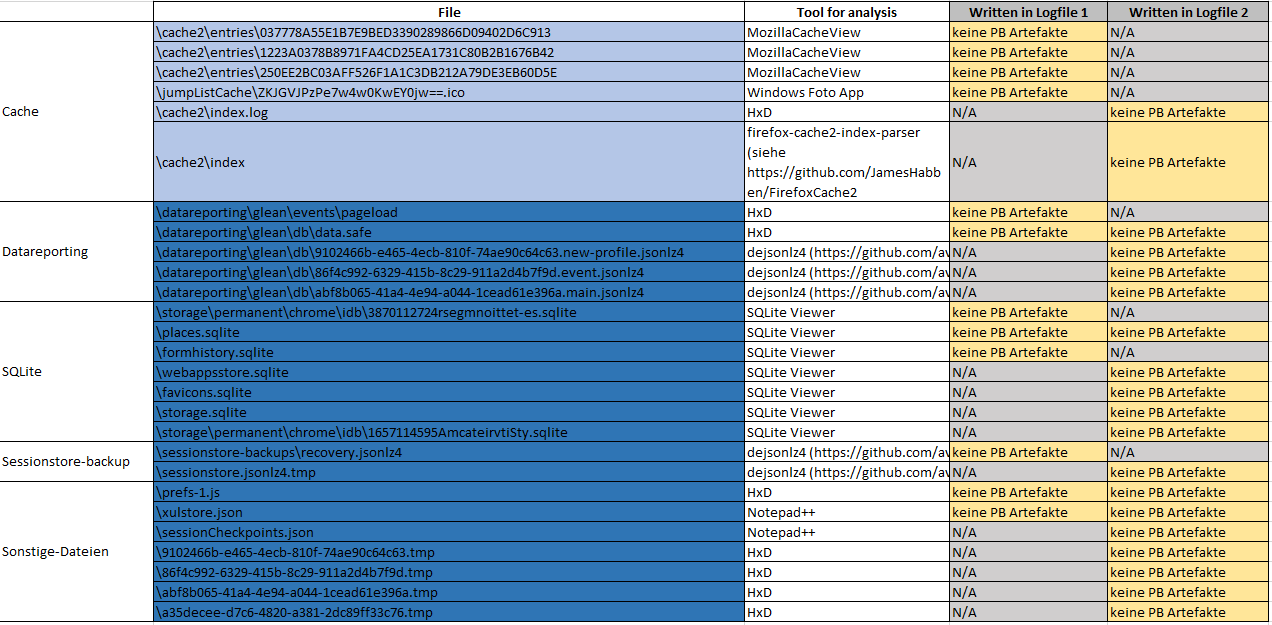
\includegraphics{bilder/firefox-tabelle-logfile1vlogfile2-reduced.png}}
%	\label{...}
	\caption{Tabelle mit wiederherstellbaren Dateien: Logfile 1 vs. Logfile 2}
\end{figure}

Allgemein: Artefakte in zwei "Common Pfaden"
-	(Local) %C:\Users\Forensik\AppData\Local\Mozilla\Firefox\Profiles\<Profile>.default-release\
-	(Roaming) %C:\Users\Forensik\AppData\Roaming\Mozilla\Firefox\Profiles\<Profile>.default-release\

Kategorien der Logs:
- Cache: 
	> % \cache2\entries\037778A55E1B7E9BED3390289866D09402D6C913 (Local)
	> % \cache2\entries\1223A0378B8971FA4CD25EA1731C80B2B1676B42 (Local)
	> % \cache2\entries\250EE2BC03AFF526F1A1C3DB212A79DE3EB60D5E (Local)
	Zweck:
		"Firefox verwendet den Cache, um Webseiten und Ressourcen wie Bilder, Stylesheets, Skripte und andere Dateien temporär auf dem lokalen Computer zu speichern. Dadurch können wiederholte Anfragen an den Server vermieden und die Ladezeiten verringert werden, da der Browser die Inhalte aus dem Cache abrufen kann, anstatt sie erneut herunterzuladen.Die tatsächlichen Inhalte dieser Datei sind binär und können je nach Art der Ressource variieren, beispielsweise HTML, Bild- oder Audiodateien."
		% https://www.techguy.org/threads/what-exactly-is-in-firefoxs-cache2-folder.1221567/
	Analyse:
		- Tool: MozillaCacheView
		- TODO: Screenshot
	> % \cache2\index (Local)
		Zweck:
			"Die Indexdatei im Cache dient als Datenbank, die Informationen über die gespeicherten Dateien enthält. Sie ermöglicht dem Firefox-Browser, schnell auf die zwischengespeicherten Ressourcen zuzugreifen und diese effizient zu verwalten"
		Analyse:
			- Tool: siehe Github und HxD
	> % \jumpListCache\ZKJGVJPzPe7w4w0KwEY0jw==.ico (Local)
		- Tool: Windows Foto App
		- Enthält kleines "m" Icon

- datareporting:
	Allgemein: "Dateien im Ordner "/datareporting/glean/db" sind Teil des Glean-Systems, das von Mozilla (dem Entwickler von Firefox) für die Sammlung von Telemetriedaten verwendet wird. Telemetrie-Daten sind anonyme Informationen über die Nutzung des Browsers, die zur Verbesserung der Software und zur Behebung von Problemen verwendet werden können. % https://github.com/mozilla/glean
	> % \datareporting\glean\db\data.safe (Roaming)	
	Zweck:
		" Die "data.safe.bin"-Datei enthält verschlüsselte Telemetrie-Daten, um ihre Integrität und Sicherheit zu gewährleisten."
	Analyse:
		- Tool: HxD
		- keine PB Artefakte
	> %  \datareporting\glean\db\<Profilname>.new-profile.jsonlz4 (Roaming)
	Zweck:
		"Diese Dateien speichern Informationen über das Firefox-Profil, das von Glean verwendet wird, um Telemetriedaten zu sammeln."
	Analyse:
		- Mit firefox propreritärem jsonlz4 Algorithmus verschlüsselt
		- können mit speziellem Tool "dejsonlz4" dekomprimiert werden (Quelle Github)
		- Dateien enthalten Systeminformationen im Json-Format (Screenshot?)

- Sessionstore-Backup:
	> % \sessionstore-backups\recovery.jsonlz4 (Roaming)
		Zweck:
			"Die Datei "recovery.jsonlz4" enthält eine Sicherungskopie der vorherigen Sitzung. Sie wird erstellt, wenn der Firefox-Browser nach einem Absturz oder einem unerwarteten Beenden neu gestartet wird." % https://support.mozilla.org/de/questions/1221836
		Analyse:
			- jsolz4 Datei in sessionstore-backup lassen sich mit Online-Tool parsen (https://www.jeffersonscher.com/ffu/scrounger.html)
			- Ergebnise: 
				Tab 1:  Willkommen bei Firefox [6.5.2023, 22:25:06, about:welcome;
				Tab 2:  Firefox Datenschutzhinweis — Mozilla [6.5.2023, 22:24:59], % https://www.mozilla.org/de/privacy/firefox/
			- Sind Seiten, die sich automatisch geöffnet haben, nachdem Firefox zum ersten Mal geöffnet wurde
			- keine PB Artefakte
	> % \sessionstore.jsonlz4
		Zweck: "Die Datei "sessionstore.jsonlz4" speichert den aktuellen Zustand der Firefox-Sitzung.  Diese Datei wird während der Browsersitzung regelmäßig aktualisiert, um sicherzustellen, dass Änderungen im Zustand der Sitzung erfasst werden."
		Analyse:
			- Lässt sich nicht mit Online-Tool aus Logfile 1 parsen
			- Stattdessen: dejsonlz4, danach Notepad++ mit JSON Plugin
			- kaum Einträge zu Sitzung, hauptsächlich CSS Daten zu Fenstergröße- und position, insb. keine PB Artefakte
			- Interessant: image-Eintrag als base64 entdeckt, in PNG umgewandelt (https://base64.guru/converter/decode/image), mit Windows Foto-App: "m" Icon (Mozilla-Logo)

- Sonstige Dateien:
	> % \prefs-1.js
		Zweck:
			"Die Datei "prefs-1.js" enthält benutzerspezifische Einstellungen und Konfigurationen für den Firefox-Browser. Sie speichert die Präferenzen des Benutzers in Form von JavaScript-Objekten.

			In dieser Datei werden verschiedene Arten von Einstellungen gespeichert, darunter:
			
		   Allgemeine Einstellungen: Dies umfasst Optionen wie die Standardsuchmaschine, die Startseite, den Zoomfaktor, die Spracheinstellungen und andere globale Einstellungen, die das Verhalten des Browsers beeinflussen.
							
		   Datenschutzeinstellungen: Hier werden Präferenzen bezüglich Cookies, Verlauf, Passwortverwaltung, Standortfreigabe und Tracking-Schutz gespeichert. Diese Einstellungen kontrollieren, wie der Browser mit persönlichen Daten und der Privatsphäre umgeht.
							
		   Add-On-Einstellungen: Wenn der Benutzer Erweiterungen oder Add-Ons installiert hat, können in dieser Datei die spezifischen Einstellungen und Konfigurationen für jedes Add-On gespeichert werden."
					% https://kb.mozillazine.org/Prefs.js_file

	> % \xulstore.json
		Zweck:
			"Die Datei "xulstore.json" speichert benutzerspezifische Anpassungen und Konfigurationen für den Firefox-Browser."
			% https://support.mozilla.org/de/kb/firefox-support-troubleshooting-guide
	Analyse:
		- Weder JSON-Dateien (Notepad++) noch .tmp Dateien (HxD) enthalten PB Artefakte
		
- SQLite: (TODO: Abgleich mit Diffs-Exceltabelle, ob wirklich nur in places.sqlite geschrieben wurde)
	Dateien haben Sonderstellung:
		- Diese DBs dienen zur Verwaltung und Speicherung sämtlicher Browser Artefakte, insb. der Browser Historie
		- Aus diesem Grund: Dateien intensiver betrachtet
	Siehe Kapitel Methodik:
		> Entwicklung von Dateiinhalt in allen Snapshots (1, 2, 3 und 4) betrachtet
		> Für jeden Snapshot: 
			- SQLite-Datei extrahiert und mit SQLite-Datei aus vorherigem Snapshot verglichen
			- Untersuchung der SQLite-Dateien mit SQLite-Viewer (GUI-Tools)
			- Wenn zu SQLite-Datei WAL-Datei existiert: mit sqlite3 Kommandozeilentool PRAGMA wal\_checkpoint durchgeführt, danach neue SQLite-Datei mit ursprünglicher SQLite-Datei verglichen
		> Dabei gibt es drei Zustände: 
			- leere Datei
			- neuer (nicht-leerer) Inhalt
			- gleichbleibender Inhalt
	Mit Process Monitor Logfiles festgestellt, dass in folgende SQLite-DBs geschrieben: 
		% https://mozilla.github.io/firefox-browser-architecture/text/0010-firefox-data-stores.html
		- places.sqlite
			"Diese Datenbank enthält Informationen über die Lesezeichen, den Verlauf und die Tags im Firefox-Browser. Sie speichert die URLs der besuchten Websites, die Zeitstempel der Besuche, die Titel der Seiten und andere relevante Daten."
		- cookies.sqlite						Speichert Webseiten-Cookies
			"In dieser Datenbank werden die Cookies gespeichert, die von Websites im Firefox-Browser verwendet werden. Cookies sind kleine Textdateien, die von Websites auf dem Computer des Benutzers abgelegt werden und verschiedene Informationen speichern können, z. B. Anmeldeinformationen, Sitzungsdaten oder Präferenzen."
		- storage.sqlite						Speicher für Webseiten
			"Diese Datenbank wird von Firefox verwendet, um verschiedene Arten von Webdaten zu speichern, wie z. B. die IndexedDB-Datenbanken von Websites, Offline-Cache-Daten, Webseiten-Skriptdaten und andere lokale Speicherinformationen."
		- favicons.sqlite						Speichert Icons für Lesezeichen
			"Diese Datenbank speichert die Favicons, also die kleinen Symbole, die in der Adressleiste und bei den Lesezeichen angezeigt werden, um Websites visuell zu identifizieren. Sie enthält die gespeicherten Favicons für die besuchten Websites."
		- webappsstore.sqlite					Speicher für Webseiten
			"Diese Datenbank speichert Informationen über installierte Webanwendungen im Firefox-Browser. Sie enthält Daten wie Berechtigungen, Einstellungen und andere spezifische Informationen für Webanwendungen."
		- formhistory.sqlite
			"In dieser Datenbank werden Informationen aus Webformularen gespeichert, die der Benutzer in Firefox ausfüllt. Sie enthält die eingegebenen Daten wie Name, E-Mail-Adresse, Adresse und andere Formulardaten, um das automatische Ausfüllen von Formularen zu ermöglichen."
		- 1657114595AmcateirvtiSty.sqlite		
			"Activity Stream for Firefox is a collection of all the things you do in the browser that you care about displayed in a rich and meaningful way" % https://wiki.mozilla.org/Firefox/Activity_Stream
		- 3870112724rsegmnoittet-es.sqlite		% https://wiki.mozilla.org/Firefox/RemoteSettings
			"Remote Settings in Firefox sind eine Funktion, die es ermöglicht, Browser-Einstellungen zentral zu verwalten und an die Benutzer zu übertragen, ohne ein vollständiges Browser-Update durchführen zu müssen."
			SQLite DB ist Datenspeicher dazu
		
	Ergebnisse:
		\begin{figure}[h!]
			\centerline{\resizebox{\linewidth}{!}{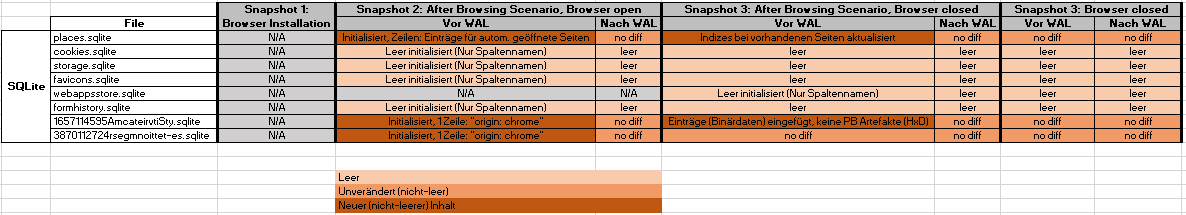
\includegraphics{bilder/firefox-sqlite-table.png}}}
			\label{chart:final-criteria}  
			\caption{Comparison of found PB artifacts between RAM Dumps}
		\end{figure}
		> Nach Browser-Installation noch keine SQLite-Datei angelegt (Snapshot 1)
		> Während Browsing Szenario alle DBs Initialisiert, außer "webappsstore.sqlite" (Snapshot 2)
			- Dabei wurden in places.sqlite die Seiten geschrieben, die sich automatisch nach Browserstart im public Modus geöffnet haben (Datenschutzhinweise zu Firefox)
			- Restliche Dateien ohne Inhalt, nur Spaltennamen
			- Nach WAL Checkpoints bleiben Dateien unverändert
		> Nach Schließen des Browsers (Snapshot 3)
			- in places.sqlite: Indizes bei eingetragenen Seiten aktualisiert
			- 1657114595AmcateirvtiSty.sqlite erhielt BLOB Eintrag, in HxD keine Muster erkennbar
			- webappsstore.sqlite: leer initialisiert, nur Spaltennamen
			- restliche Dateien unverändert
			- nach WAL Checkpoints bleiben Dateien unverändert
		> Nach herunterfahren der VM (Snapshot 4)
			- Alle Dateien unverändert, auch nach WAL Checkpoint
	
- Zusammenfassung: in keiner Datei PB Artefakte

Quantitativ: (Diagramme)		
	> Balkendiagramm: Für jede Logfilekategorie: Anzahl Schreiboperationen Logfile 1 vs Logfile 2
	\begin{figure}[h!]
		\centerline{\resizebox{\linewidth}{!}{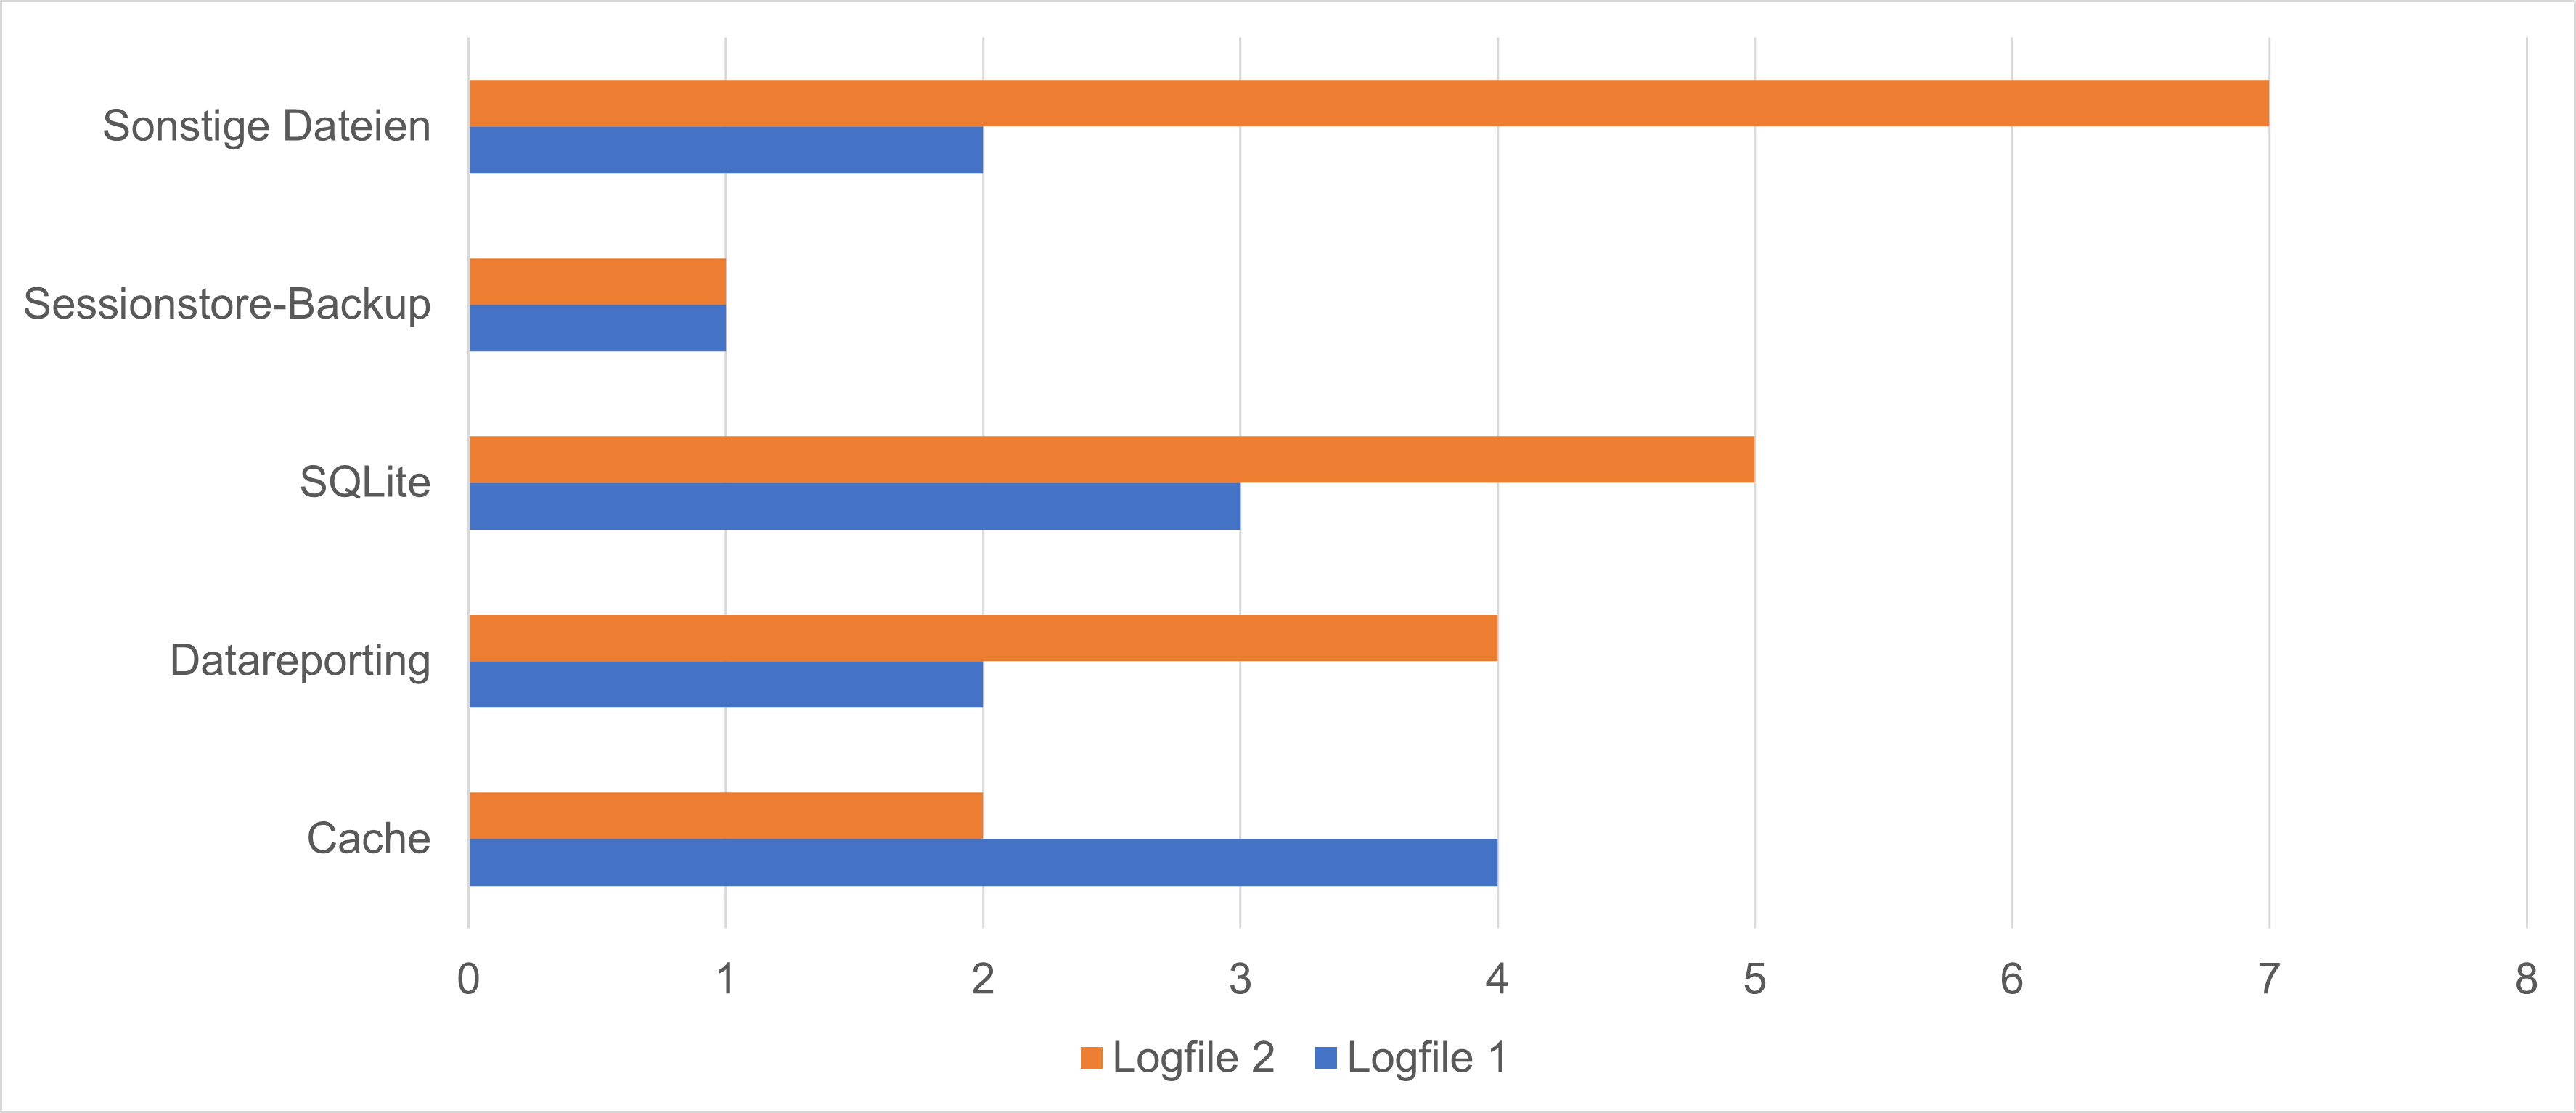
\includegraphics{bilder/bar-chart-logfile1vs2-test.png}}}
		\label{chart:final-criteria}  
		\caption{Comparison of found PB artifacts between RAM Dumps}
	\end{figure}

%Literatur:
%	o no traces were found in “common locations” \cite{Montasari.2015}
%		>  “places.sqlite”, “webappsstore. sqlite”, “sessionstore.bak”, “search.json” and “nssckbi.dll”
%	o	Safebrowsing: Alle Dateien in /safebrowsing-updating/ nicht relevant. Dort nur .vlpset und .sbstore Dateien. Speichern 256-Bit Hash von URLs, die auf SafeSearch Blacklist stehen 
%	o	Cache-Dateien: drei Caches: startupCache, jumpListCache (beide enthalten Binärdateien ohne Browsing Artefakte) und cache2 (können mit MozillaCacheView untersucht werden, enthalten keine Browsing Artefakte)
%	o	SQLite Datenbanken: Sqlite Dateien erst ohne WAL Dateien untersuchen, Danach mit sqlite3 Konsole: WAL in Datenbank schreiben mit: PRAGMA wal\_checkpoint; places.sqlite besonders relevant, da dort Browser in public Modus Browsing URLs verwaltet (Am besten hier vergleich mit Public Browsing machen)	
%		> \cite{Fayyad.2021} for Mozilla Firefox, 7 database files were recovered: cookies.sqlite-shm, places.sqlite-shm, prefs.js etc.
%		> \cite{Muir.2019} The two SQLite databases used by Firefox to track cookies and history (cookies.sqlite und places.sqlite) were both recoverable from the file system after deletion	
%		Ergebnisse stehen im Gegensatz zu \cite{Hedberg.2013} :
%			o	Chrome und Firefox: Einträge in places.sqlite + history.sqlite DB gefunden während PB! (Noch aktuell??)
%		Sonderfall: SQlite DB-Crash \cite{Hedberg.2013}
%			> WAL Files/Journal Files bei Crash gefunden -> Kann genutzt werden um zu beweisen, dass privater Browser genutzt wurde
%			> Daher: WAL Rollback mit sqlite3	
%	o	Jsonlz4 \& balkz4: Enthalten komprimierte Firefox-Sessions, jsonlz4 Dateien können mit Tool "entkomprimiert" werden: https://www.jeffersonscher.com/ffu/scrounger.html


\subsection*{Registry}
> Process Monitor: SetValue Operationen von Browser 
TODO: Logfile 1 vs 2?
	Kategorien Registry Keys:
	1) PreXULSkeletonUISettings:
		> Prefix: Absoluter Installationspfad von Firefox
		> Skeleton UI Einstellungen von Firefox % https://itigic.com/skeleton-ui-new-firefox-interface-to-start-up-much-faster/#google_vignette
			Definition:
				> Der "PreXULSkeletonUISettings" Registry Key enthielt Einstellungen für die Benutzeroberfläche (UI) des Firefox-Browsers, insbesondere für das sogenannte "Skeleton UI". Das Skeleton UI ist eine vereinfachte Benutzeroberfläche, die während des Ladens des Browsers angezeigt wird, bevor die vollständige Benutzeroberfläche geladen ist. Es besteht aus grundlegenden Steuerelementen und Elementen, die dem Benutzer die Interaktion ermöglichen, während der Rest der Benutzeroberfläche noch geladen wird.
				> Der "PreXULSkeletonUISettings"-Schlüssel enthielt Konfigurationsoptionen wie Farben, Positionen und andere Einstellungen für das Skeleton UI. Durch das Bearbeiten dieses Schlüssels konnten Benutzer die Darstellung des Skeleton UI anpassen. Es ist jedoch wichtig zu beachten, dass das Ändern der Registrierungseinträge ein fortgeschrittenes Verfahren ist und Fehler zu Problemen mit dem Browser führen kann.
			
		> Struktur der Keys: % HKCU\SOFTWARE\Mozilla\Firefox\PreXULSkeletonUISettings\C:\Program Files\Mozilla Firefox\firefox.exe|<UI Einstellung>
		> Unterschiedliche UI Einstellungen
			- % ScreenX (DWORD)
			- % ScreenY (DWORD)
			- % Width (DWORD)
			- % Height (DWORD)
			- % Maximized (DWORD)
			- % Flags (DWORD)
			- % CssToDevPixelScaling (REG_BINARY)
			- % UrlbarCSSSpan (REG_BINARY)
			- % SearchbarCSSSpan (REG_BINARY)
			- % SpringsCSSSpan (REG_BINARY)
		> keine PB Artefakte unter UI Einstellungen	
	2) Business Activity Monitoring % https://learn.microsoft.com/de-de/biztalk/core/business-activity-monitoring-bam
		> Quelle: % https://notes.qazeer.io/dfir/windows/_artefacts_overview
		> BAM is a mostly undocumented feature that controls the programs executed in the background. DAM is a feature for devices supporting the "Connected Standby" mode (i.e when a device is turned on, but its display will be turned off). As a result, the BAM registry keys will contain data on any devices, while DAM registry keys will only contain data on mobile devices.
		> The BAM registry key contains multiple subkeys under bam\\State\\UserSettings, with one subkey per user, identified with the user SID. While the key is in the SYSTEM registry hive, program executions can thus still be tied to a specific user using this SID.
		> Each user-specific key contains a list of executed programs, with their full path and timestamp of last execution.
		> If a file is deleted, the eventual associated entry in the BAM is deleted as well after the system reboot. Additionally, BAM entries older than 7 days are deleted upon system boot. The BAM thus provides limited information on historic execution of programs
		> No entries are created in the BAM keys for executables on removable media and/or on network shares.
		> Key: %  HKLM\System\CurrentControlSet\Services\bam\State\UserSettings\S-1-5-21-588412547-2749917301-3803556669-1001\\Device\HarddiskVolume2\Program Files\Mozilla Firefox\firefox.exe (REG_BINARY)

Quantitativ: (Diagramme)
	- Stacked Balkendiagramm jeweils für Logfile 1 und Logfile2: Anteil Kategorie 1 bzw.2 an allen Registry-Schreiboperationen
	\begin{figure}[h!]
		\centerline{\resizebox{\linewidth}{!}{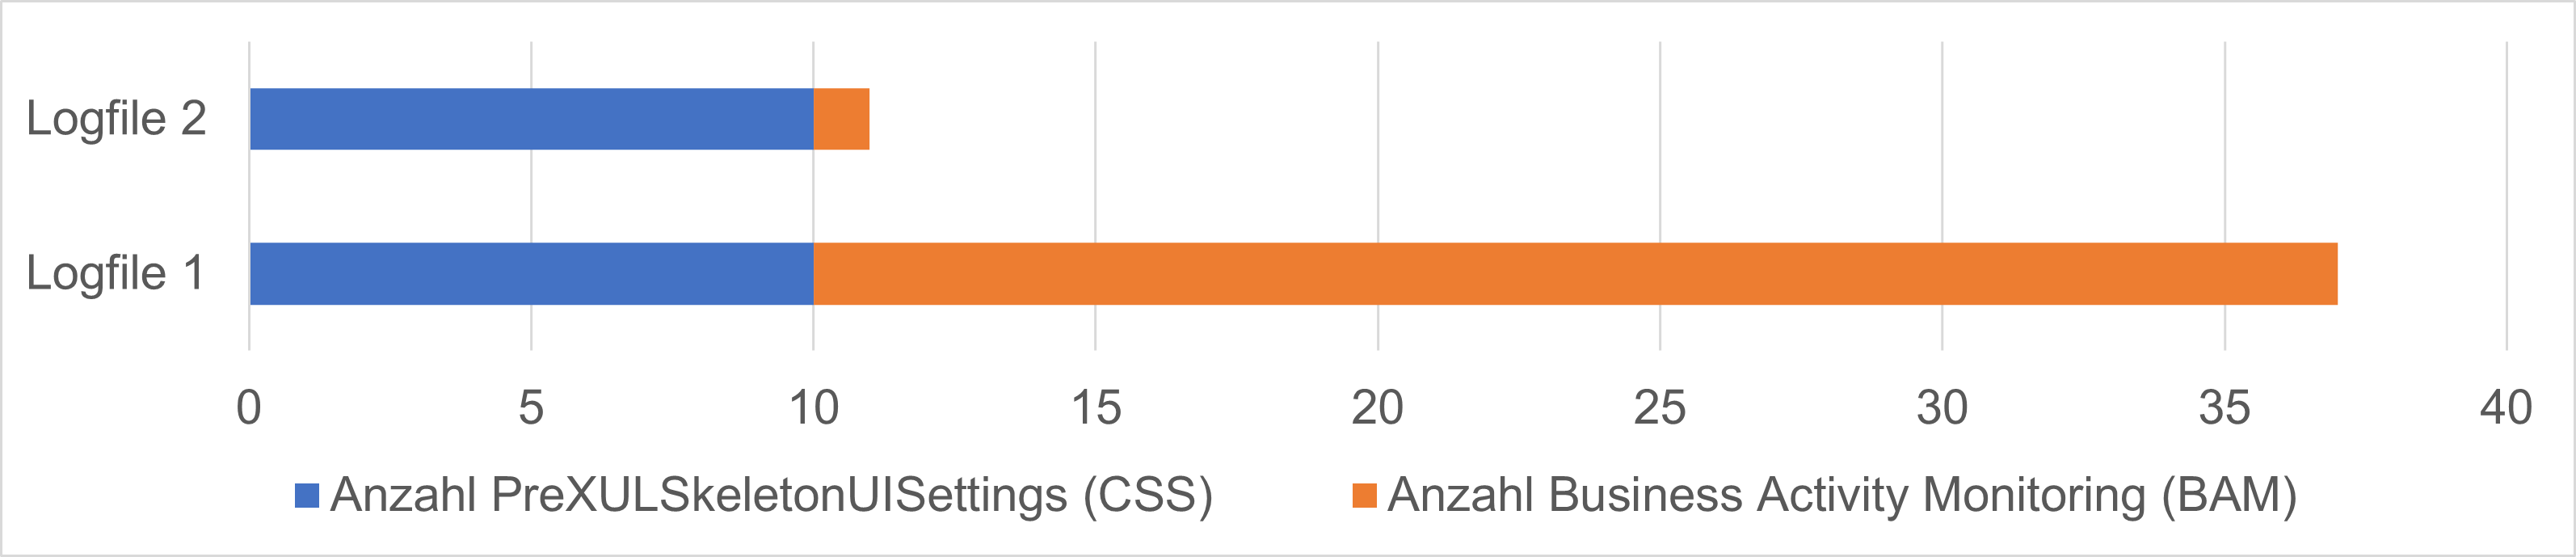
\includegraphics{bilder/firefox-registry-stacked-bar-chart.png}}}
		\label{chart:final-criteria}  
		\caption{Comparison of found PB artifacts between RAM Dumps}
	\end{figure}
	
> Stringsuche in Registry Hives mit Registry Explorer (Siehe Liste)
	In allen Hives kein Treffer für alle Suchbegriffe

Literatur: 
	> angeblich in Shellactivities Ergebnisse. --> Nicht mehr vorhanden in aktueller Version (Verweis auf E-Mail)

%Literatur:
%	>	Auf Autor verweisen: angeblich in Shellactivities Ergebnisse. --> Nicht mehr vorhanden in aktueller Version (Verweis auf E-Mail)
%	>	Process Monitor/Regshot zeigen keine relevanten Key-Änderungen
%	> \cite{Muir.2019}: Autopsy Keyword Suche nach Suchbegriffen: Ergebnisse in \%SystemRoot\%Minidump NTUSER.DAT, ntuser.dat.LOG1 (a log of changes to NTUSER.DAT)
%	> Zentral: shellactivites Key:	NTUSER.DAT --> “shellactivities” key \cite{Muir.2019}
%	> \cite{Rochmadi.2017} Detection of registry changes helps to determine what the appropriate plugin is used to search for digital evidence using volatility memory forensic:
%	- RegQueryValue:	HKCU/Software/Microsoft/Windows/CurrentVersion/InternetSettings/Connections/DefaultConnectionSettings
%	- RegCloseValue: 	HKCU/Software/Microsoft/Windows/CurrentVersion/InternetSettings/Connections
%	- IRP\_MJ\_READ: C:/pagefile.sys

\subsection*{Black-Box Analyse/Uncommon Locations}

\subsubsection*{Analyse mit Autopsy}
Bei White-Box Analyse/Common Locations: Autopsy nur zur Dateiextraktion genutzt, hier: als konkretes forensisches Werkzeug

Stichwortsuche:
- In allen Snapshots keine Treffer (auch innerhalb \$Carved)
- TODO: Pagefile gefunden?

Von Autopsy automatisch indexierte Dateien: 
In allen Fällen: keine Dateien gelöscht, nur über Zeitraum der Snapshots neue dazugekommen
- Web Bookmarks:
	\begin{figure}[h!]
		\centerline{\resizebox{\linewidth}{!}{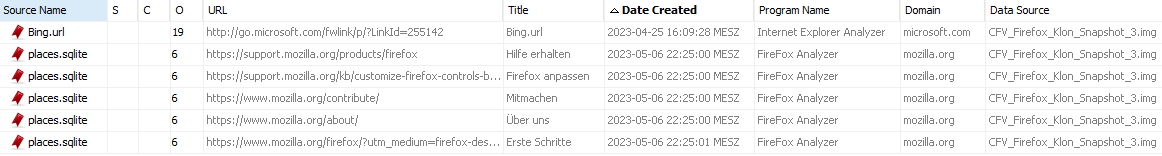
\includegraphics{bilder/cfv_firefox_autopsy_web_bookmarks.png}}}
		\label{chart:final-criteria}  
		\caption{Autopsy Web Bookmarks}
	\end{figure}
	Snapshot 1:
		> Bing.url (Unter C:/User/Forensik/Favorites/Links) enthält Bing Startseite
	Snapshot 2:
		> 5 Einträge in places.sqlite: (Firefox Standardseiten -> Deckt sich mit Beobachtungen aus Process Monitor Analyse, siehe Kapitel X)
	Snapshot 3:
		> unverändert zu 2
	Snapshot 4:
		> unverändert zu 3
- Web Cookies:
	\begin{figure}[h!]
		\centerline{\resizebox{\linewidth}{!}{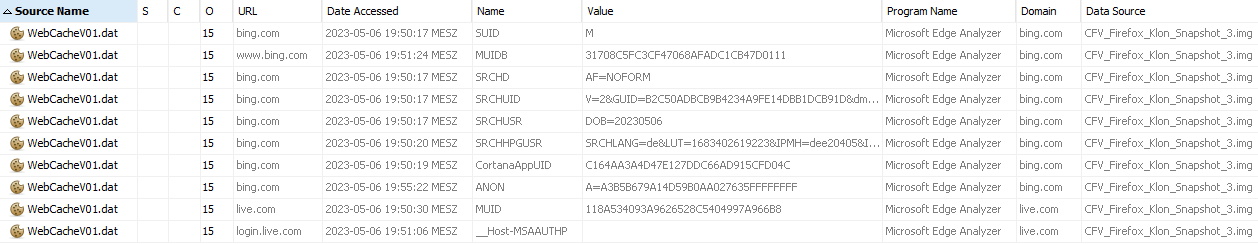
\includegraphics{bilder/cfv_firefox_autopsy_web_cookies.png}}}
		\label{chart:final-criteria}  
		\caption{Autopsy Web Cookies}
	\end{figure}
	Snapshot 1:
		> 10 Einträge in WebCacheV01.dat (= DB des Internet Explorers zum speichern von Browserdaten): Cookies für bing.com und live.com (= outlook)
	Snapshot 2:
		> unverändert zu 1
	Snapshot 3:
		> unverändert zu 2
	Snapshot 4:
		> unverändert zu 3
- Web History:
	\begin{figure}[h!]
		\centerline{\resizebox{\linewidth}{!}{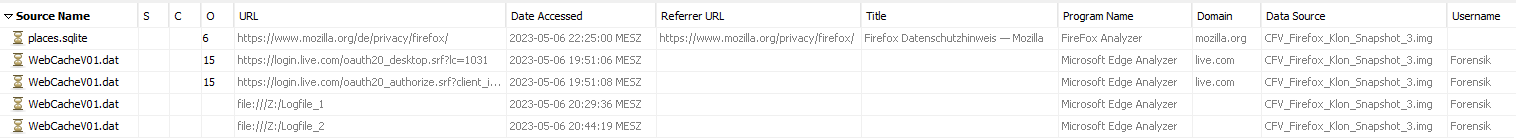
\includegraphics{bilder/cfv_firefox_autopsy_web_history.png}}}
		\label{chart:final-criteria}  
		\caption{Autopsy Web History}
	\end{figure}
	Snapshot 1:
		> 2 Einträge in WebCacheV01.dat:
			- 2x live.com (= outlook)
	Snapshot 2:
		> 1 Eintrag in places.sqlite: % https://www.mozilla.org/privacy/firefox/
			-> Zurückzuführen auf Seite, die sich automatisch geöffnet hat, als Firefox gestartet (bevor privates Fenster geöffnet wurde)
		> 1 neuer Einträge in WebCacheV01.dat:
			- file:///Z:/Logfile\_1 (= Process Monitor Logfile, die in shared-Folder geladen wurde) -> Erklärung?
	Snapshot 3:
		> 1 neuer Eintrag in WebCacheV01.dat:
			- file:///Z:/Logfile\_2 (= Process Monitor Logfile, die in shared-Folder geladen wurde) -> Erklärung?
	Snapshot 4:
		> unverändert zu 3
- Web Categories:
	\begin{figure}[h!]
		\centerline{\resizebox{\linewidth}{!}{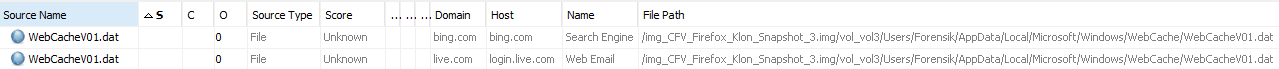
\includegraphics{bilder/cfv_firefox_autopsy_web_categories.png}}}
		\label{chart:final-criteria}  
		\caption{Autopsy Web Categories}
	\end{figure}
	Snapshot 1:
		> 2x WebCacheV01.dat aufgelistet => Mit HxD untersucht, keine PB Artefakte
	Snapshot 2:
		> unverändert zu 2
	Snapshot 3:
		> unverändert zu 3
	Snapshot 4:
		> unverändert zu 4
		
Zusammenfassung:
- keine PB Artefakte
- Keine neuen Erkenntnisse vgl. mit intensiver Analyse mittels Process Monitor in Kapitel X
- Eintrag von Datenschutzseite in places.sqlite wurde erkannt.

%Literatur:
%	o	Autopsy Keywortsuche: 
%		>	In alles Snapshots ergebnislos (keine Keyword-Hits
%		-->	In Literatur: Autoren fanden Ergebnisse in pagefile.sys 
%			> Autopsy: websites and some of the keywords found in hidden file called “pagefile.sys” \cite{Mahlous.2020}
%			o \cite{Montasari.2015} traces were found in: 
%				> However, on investigating the “pagefile.sys”, some entries were discovered
%				> Using the “data carving” technique, profile picture was recovered
%			o \cite{Said.2011} 
%				> Examining pagefile.sys showed some positive hits 			
%		--> Evtl. hier zeigen, was gefunden werden kann, wenn RAM reduziert
%		--> Aber auf Problem hinweisen, dass gefundener String in pagefile nicht direkt Browser zugeordnet werden kann
%		> \cite{Gabet.2018}	Firefox only produced three recoverable artefacts as reported by both tools (FTK, Autopsy) --> Artefakte werden nicht genannt!
%		> \cite{Muir.2019} Autopsy Keyword Suche nach Suchbegriffen: unallocated space
%		> Autopsy Carving Module (\$Carved): \cite{Muir.2019}
%			•	When searching for the string ’clot’ from the browsing protocol, six .dll, .edb and .reg files were discovered in unallocated space.
%			•	Further searching of unallocated space uncovered references to the Tor installation directory and the obfs4 bridging IP addresses
%			•	browsing data found in NTUSER.DAT was also replicated in unallocated space.
%	o	Autopsy PlugIns:
%		>	*** TODO: Hier Liste mit PlugIns ***

\subsubsection*{Analyse mit Volatility}
Vorgehen: Siehe "Methodik" Kapitel
	- Ausgangslage: Volatility Yarascan Treffer
	- Für jeden Treffer: virtueller Offset des Strings, PID, getriggerte Yararule, getriggerte Yara Component z(= Variablenname des gesuchten Strings), gefundener String
	- Neue Spalte: "Prozessname" -> zu jeder PID Prozessnamen
	- Ergebnisse Aufbereitet nach folgendem Schema:
		> Für jeden RAM Dump
		> Für jede Yararule
		> Für jede Component
		> Filter: Prozessname = Firefox -> Anzahl zählen
		> Filter: Prozessname = Alle Prozesse außer Firefox -> Anzahl zählen

HTML Artefakte wurden in keinem RAM Dump gefunden => Nicht aufgeführt

Yararule "Keyword":
	\begin{figure}[h!]
		\centerline{\resizebox{\linewidth}{!}{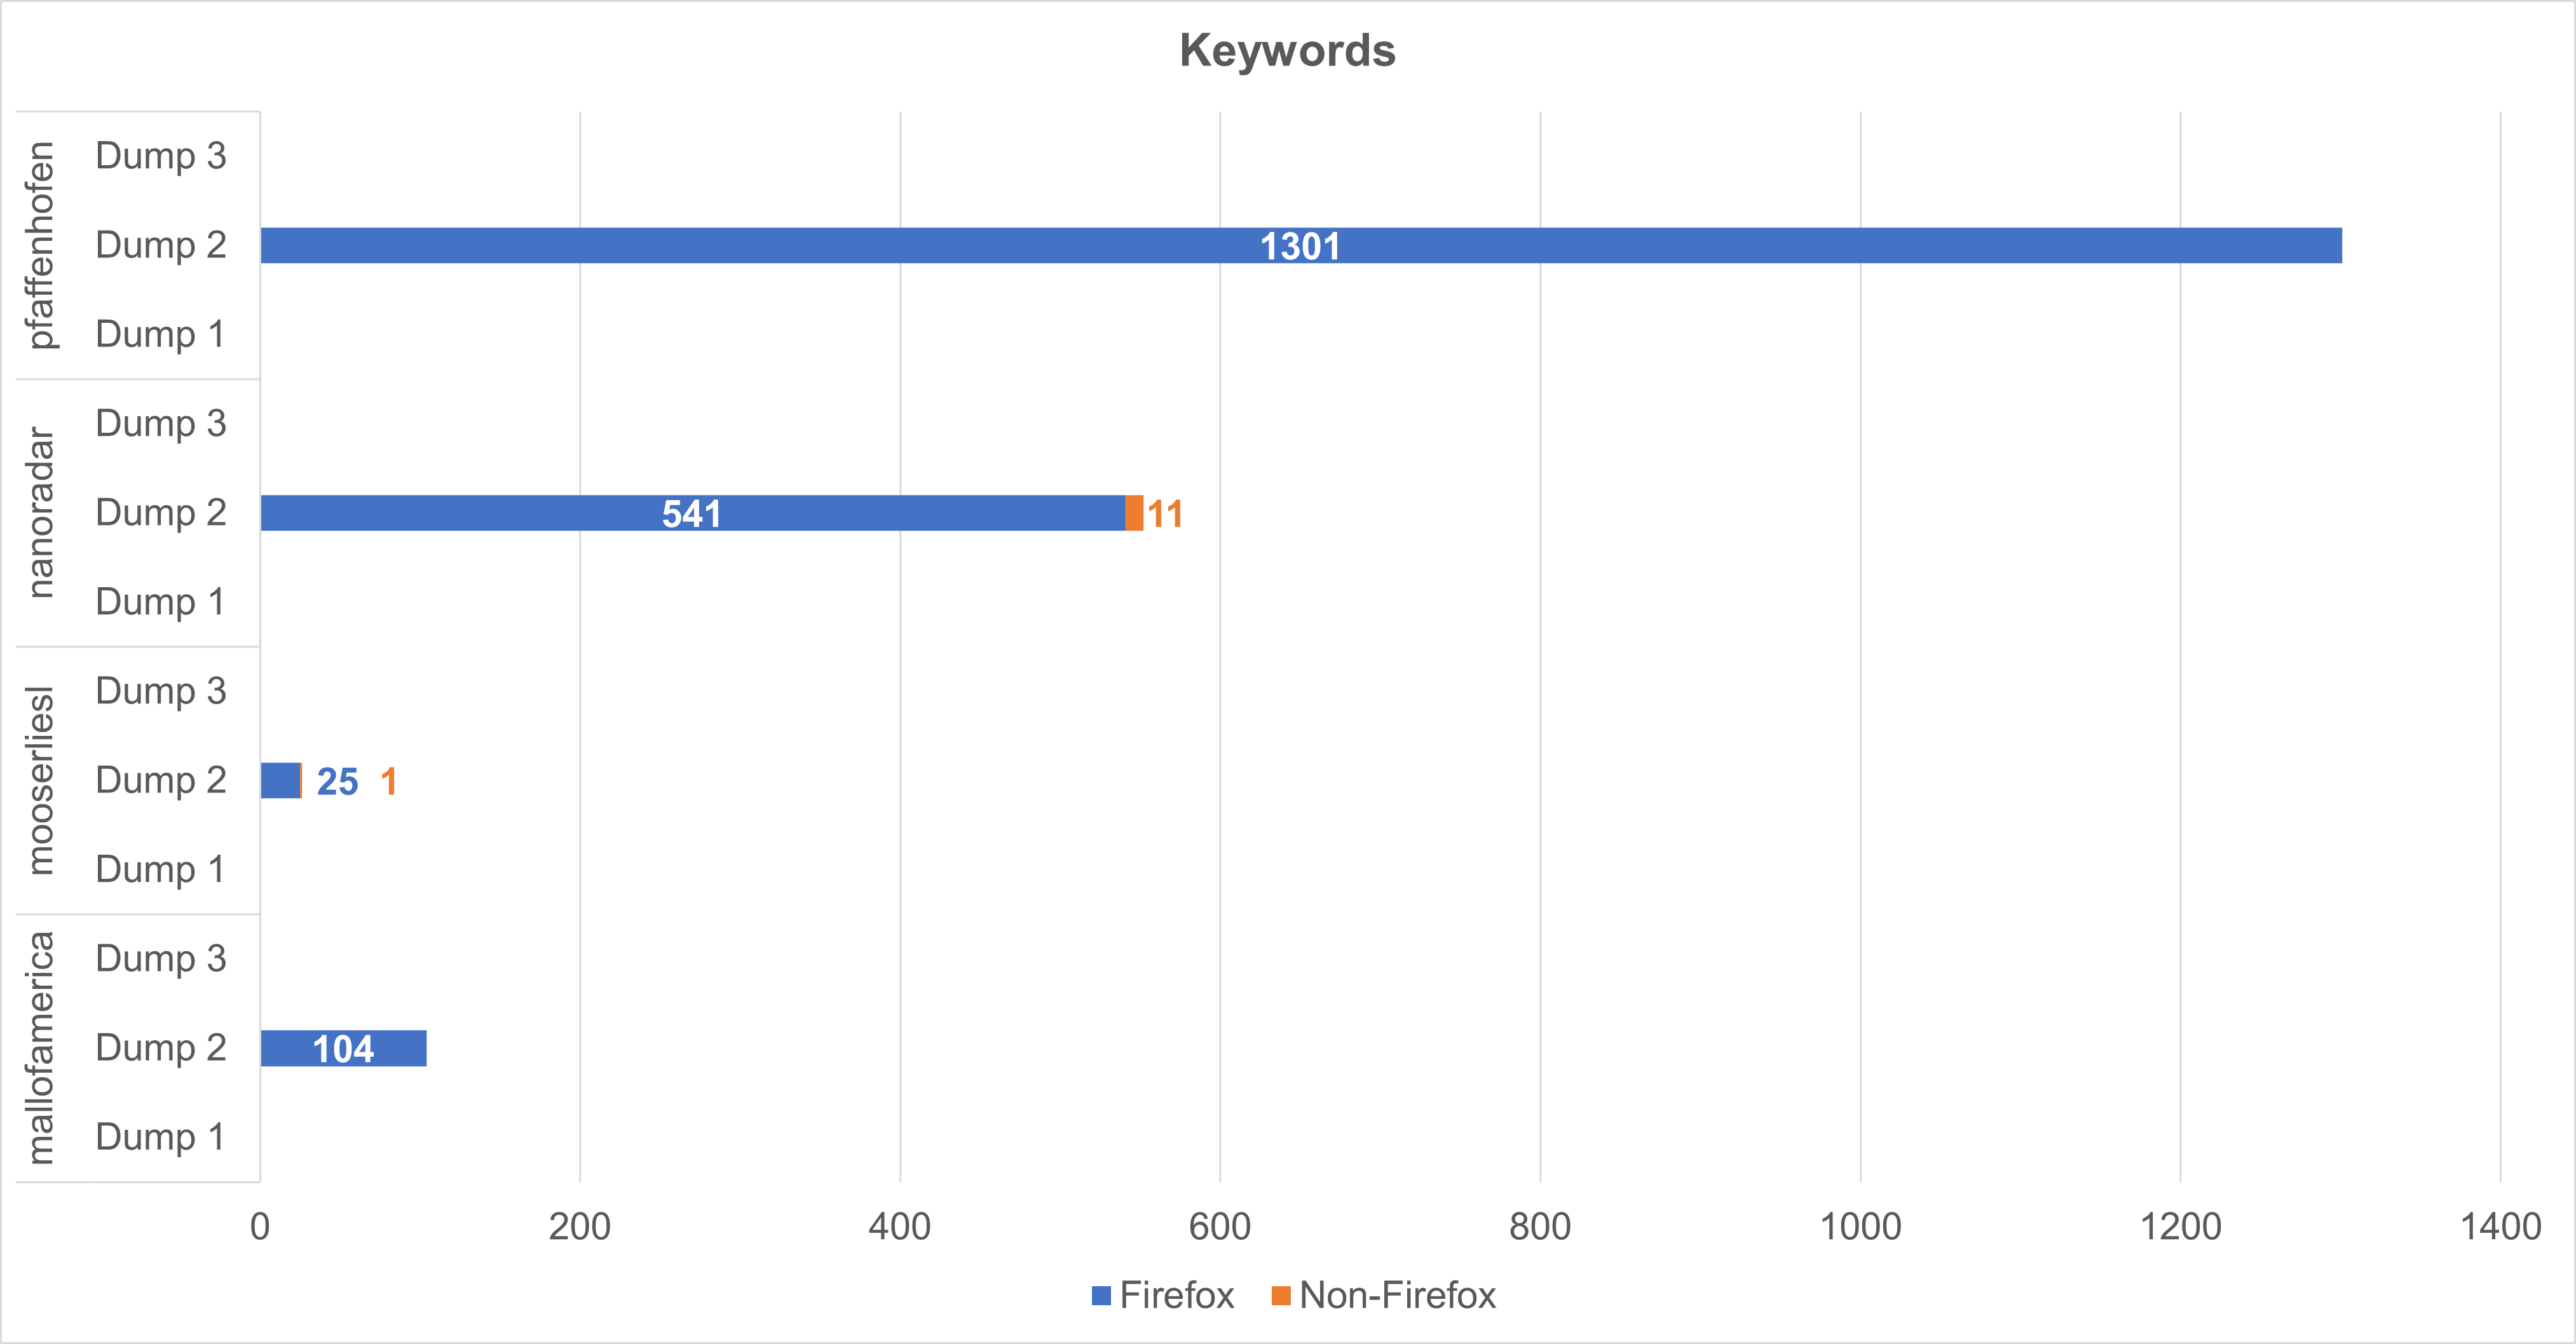
\includegraphics{bilder/volatility/firefox/keywords.png}}}
		\label{chart:final-criteria}  
		\caption{Keywords}
	\end{figure}
	Analyse:
		> Ausschließlich in RAM Dump 2 Keyword Artefakte gefunden
		> Hauptsächlich in Firefox Prozess
		> Mit 1301 Artefakten, am häufigsten pfaffenhofen vertreten. Vermutung: Evtl. weil Google Maps viele zusätzliche Artefakte lädt. 
		
Yararule "URL":
	\begin{figure}[h!]
		\centerline{\resizebox{\linewidth}{!}{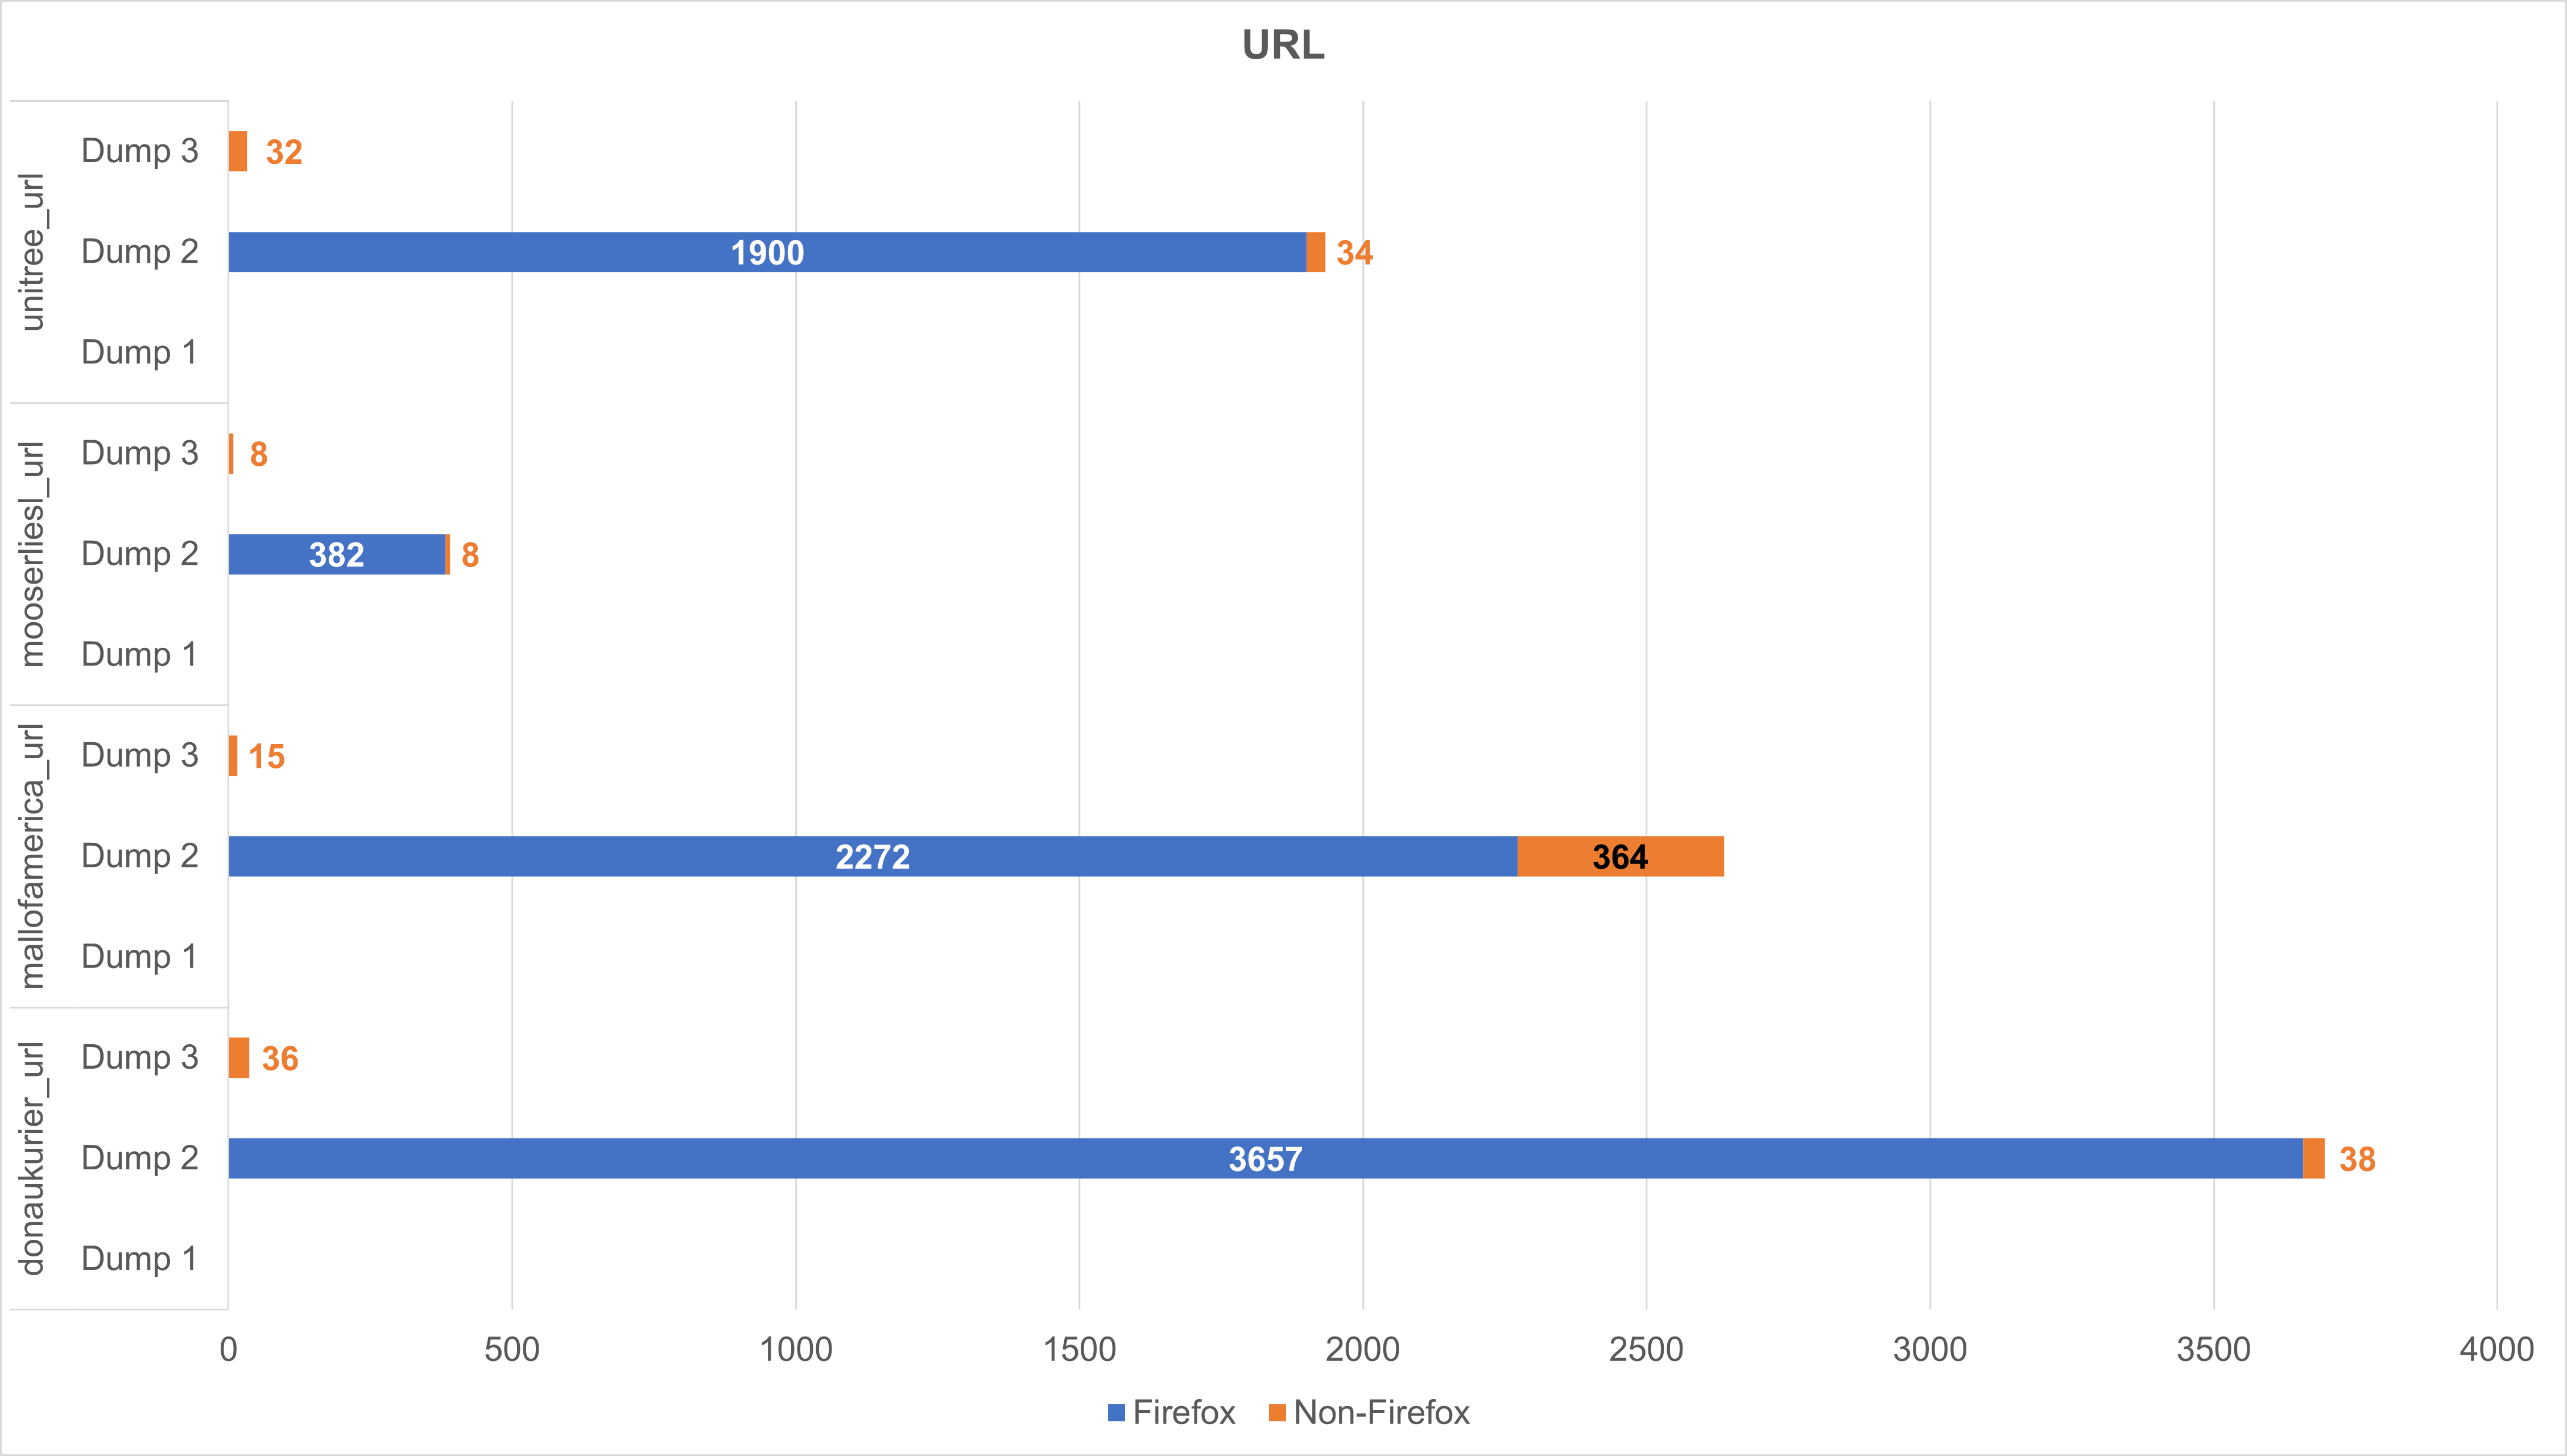
\includegraphics{bilder/volatility/firefox/url.png}}}
		\label{chart:final-criteria}  
		\caption{URL}
	\end{figure}
	Analyse:
		> Wie bei anderen Kategorien: Die meisten Artefakte in RAM Dump 2, in Firefox Prozessen
		> mooserliesl tritt am wenigsten auf, donaukurier am meisten (vmtl. auf Öffnen von Bild zurückzuführen)
		> Hier bemerkenswert, dass in RAM Dump 3 Artefakte von allen vier URLs zu finden sind
		> Bei genauerer Analyse des Process Monitor Logfiles herausgefunden: Artefakte alle in svchost.exe Prozess gefunden
		> Deshalb RAM Dump erneut mit Volatility windows.svcscan Plugin untersucht:
			"The svcscan plugin allows the analyst to list out the services running. This plugin gives more detail to the running processes in the event that the analyst requires additional details such as the display name, binary path, or service type." % (https://www.oreilly.com/library/view/digital-forensics-and/9781787288683/9ab60586-2b04-45e0-b437-dbfe10ab3be8.xhtml)
		> Ausgabe aller im RAM gefundener Services
		> Problem: Volatility svcscan liefert keine PID zu laufenden Services
		> Deshalb: "White-Box" Analyse: Snapshot 3 erneut aufgetaut, danach mit Process Explorer PID X (TODO!) von SVChost Prozess gesucht, in dem PB Artefakte gefunden wurden
			Def. Process Explorer:
				"Prozess Explorer zeigt Ihnen Informationen darüber an, welche Handles und DLLs-Prozesse geöffnet oder geladen wurden." % https://learn.microsoft.com/de-de/sysinternals/downloads/process-explorer
				"Process Explorer, from Sysinternals, is a process management program that allows you to see the running processes on your computer and a great deal of information about each process. One of the nice features of Process Explorer is that it also gives you the ability to see what services a particular SVCHOST.EXE process is controlling."
		> Ergebnis: DNSCache Service mit PID X (TODO!) = DNScache Service
			TODO: Screenshot
		> Ausführung von ipconfig /displaydns liefert gecachte URLs
			TODO: Screenshot
		> Nach Löschen des DNSCaches mit ipconfig /flushdns + Schließen aller Process Monitor Instanzen + Beenden des DNSCaches Services + Erneuter RAM-Dump -> Keine PB Artefakte mehr gefunden!
Yararule "Mail":
	\begin{figure}[h!]
		\centerline{\resizebox{\linewidth}{!}{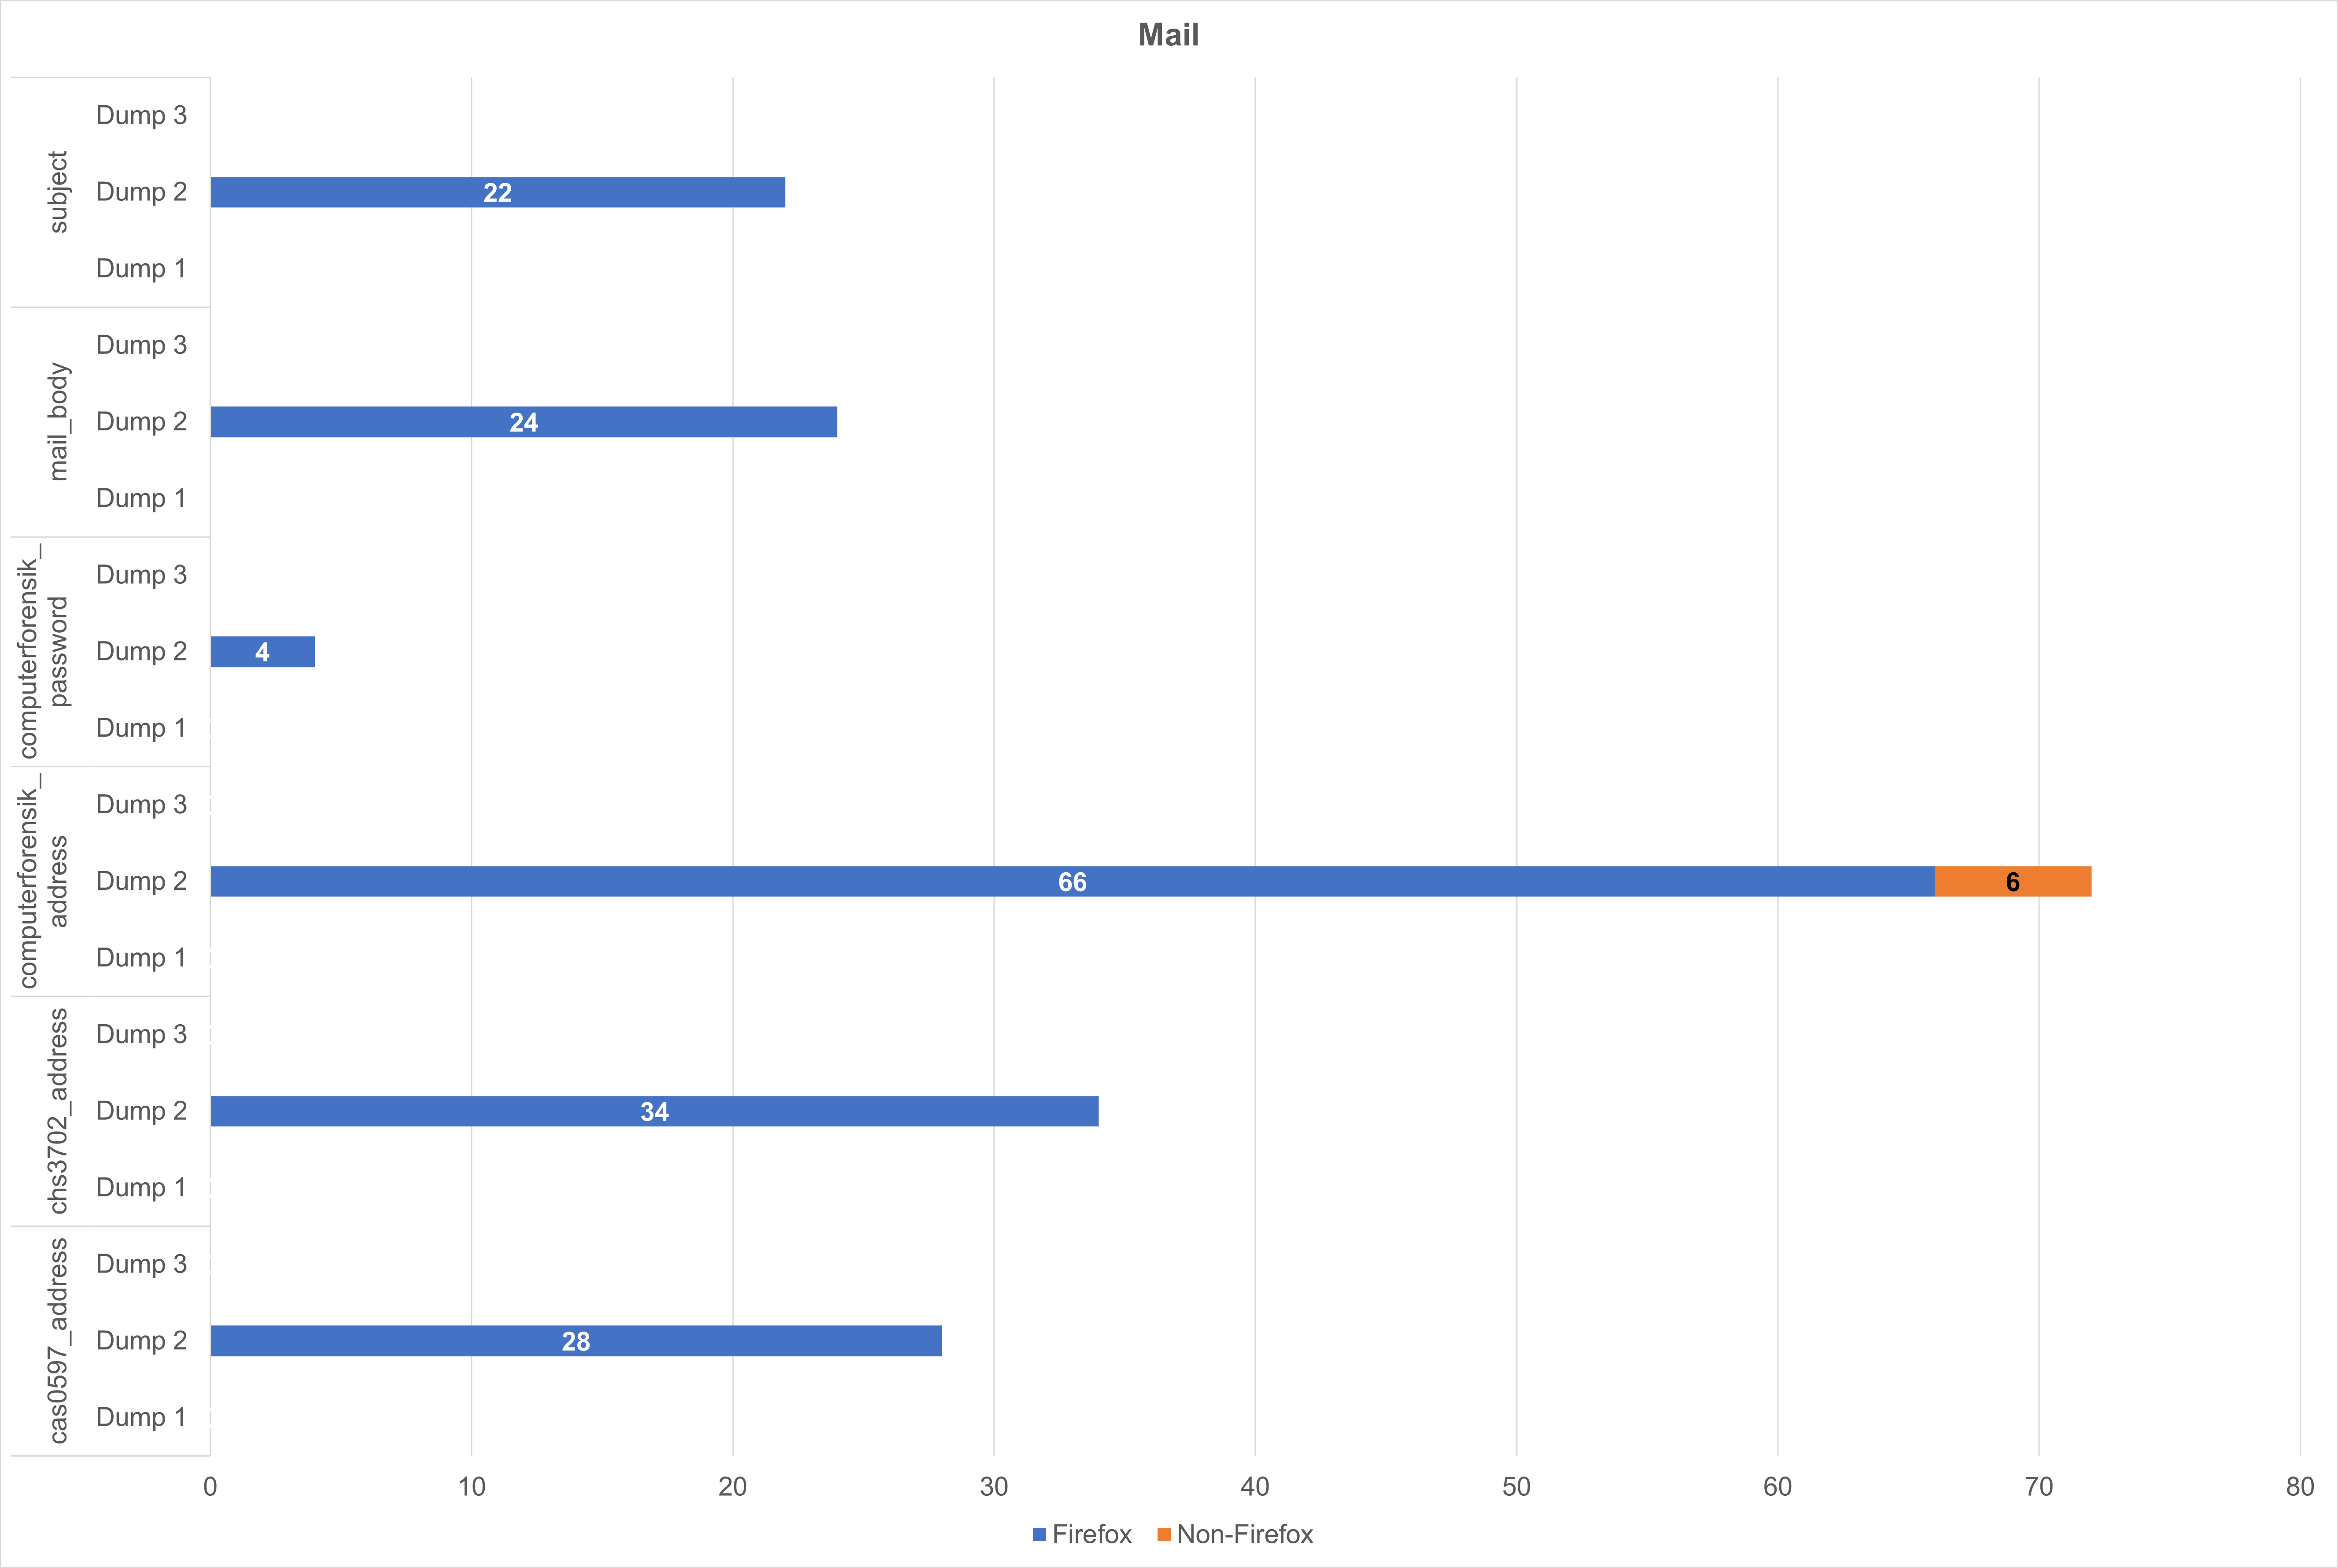
\includegraphics{bilder/volatility/firefox/mail.png}}}
		\label{chart:final-criteria}  
		\caption{Mail}
	\end{figure}
	Analyse:
		> Alle Mail Artefakte gefunden
		> Ausschließlich in RAM Dump 2 Mail Artefakte gefunden
		> Am häufigsten Absenderadresse "computerforensikvl@gmail.com" gefunden, als einziges Artefakt auch in anderen Prozessen gefunden.
		> Bemerkenswert: Passwort wurde 4x als Klartext im RAM gefunden!
			String Kontext:
				Offsets:		PIDs:
				0xb9ce29180c8	7420
				0x2859f4ffd4e0	7420
				0x24083b41858	8424
				0x240840e5b08	8424
				
			Memmap: Pid 7420
				virtual			physical	size	offset in file
				0xb9ce2918000	0xcb20a000	0x1000	0x11dd4000
					-> 0xb9ce29180c8 = 0x11dd40c8 
					\begin{figure}[h!]
						\centerline{\resizebox{0.7\linewidth}{!}{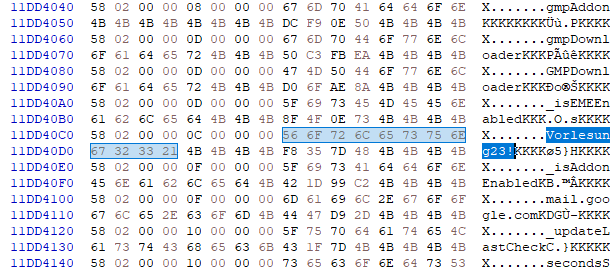
\includegraphics{bilder/volatility/firefox/password_0xb9ce29180c8_7420.png}}}
						\label{chart:final-criteria}  
						\caption{Password in memory page of PID 7420 at offset 0xb9ce29180c8}
					\end{figure}
				0x2859f4ffd000	0x96812000	0x1000	0x12e23000	Disabled				
					-> 0x2859f4ffd4e0 = 0x12e234e0
					\begin{figure}[h!]
						\centerline{\resizebox{0.7\linewidth}{!}{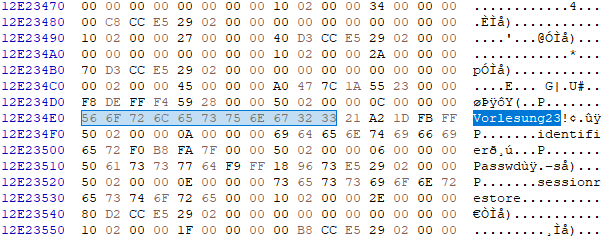
\includegraphics{bilder/volatility/firefox/password_0x2859f4ffd4e0_7420.png}}}
						\label{chart:final-criteria}  
						\caption{Password in memory page of PID 7420 at offset 0x2859f4ffd4e0}
					\end{figure}
			Memmap: Pid 8424
				virtual			physical	size	offset in file
				0x24083b41000	0xc1d52000	0x1000	0x583000	Disabled
					-> 0x24083b41858 = 0x583858
					\begin{figure}[h!]
						\centerline{\resizebox{0.7\linewidth}{!}{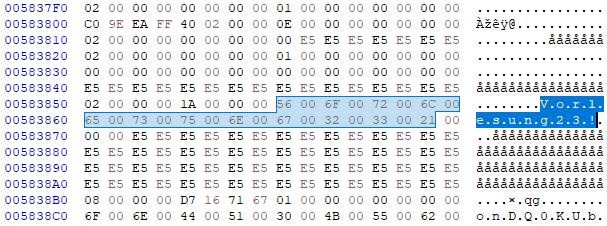
\includegraphics{bilder/volatility/firefox/password_0x24083b41858_8424.png}}}
						\label{chart:final-criteria}  
						\caption{Password in memory page of PID 8424 at offset 0x24083b41858}
					\end{figure}
				0x240840e5000	0x2d3fb000	0x1000	0x96b000	Disabled
					-> 0x240840e5b08 = 0x96bb08
					\begin{figure}[h!]
						\centerline{\resizebox{0.7\linewidth}{!}{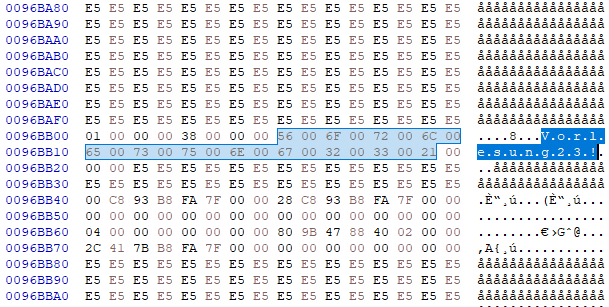
\includegraphics{bilder/volatility/firefox/password_0x240840e5b08_8424.png}}}
						\label{chart:final-criteria}  
						\caption{Password in memory page of PID 8424 at offset 0x240840e5b08}
					\end{figure}
		> In PID 8424: 2 Bytes pro Character, bspw. Unicode
				
Yararule "Image":
	\begin{figure}[h!]
		\centerline{\resizebox{\linewidth}{!}{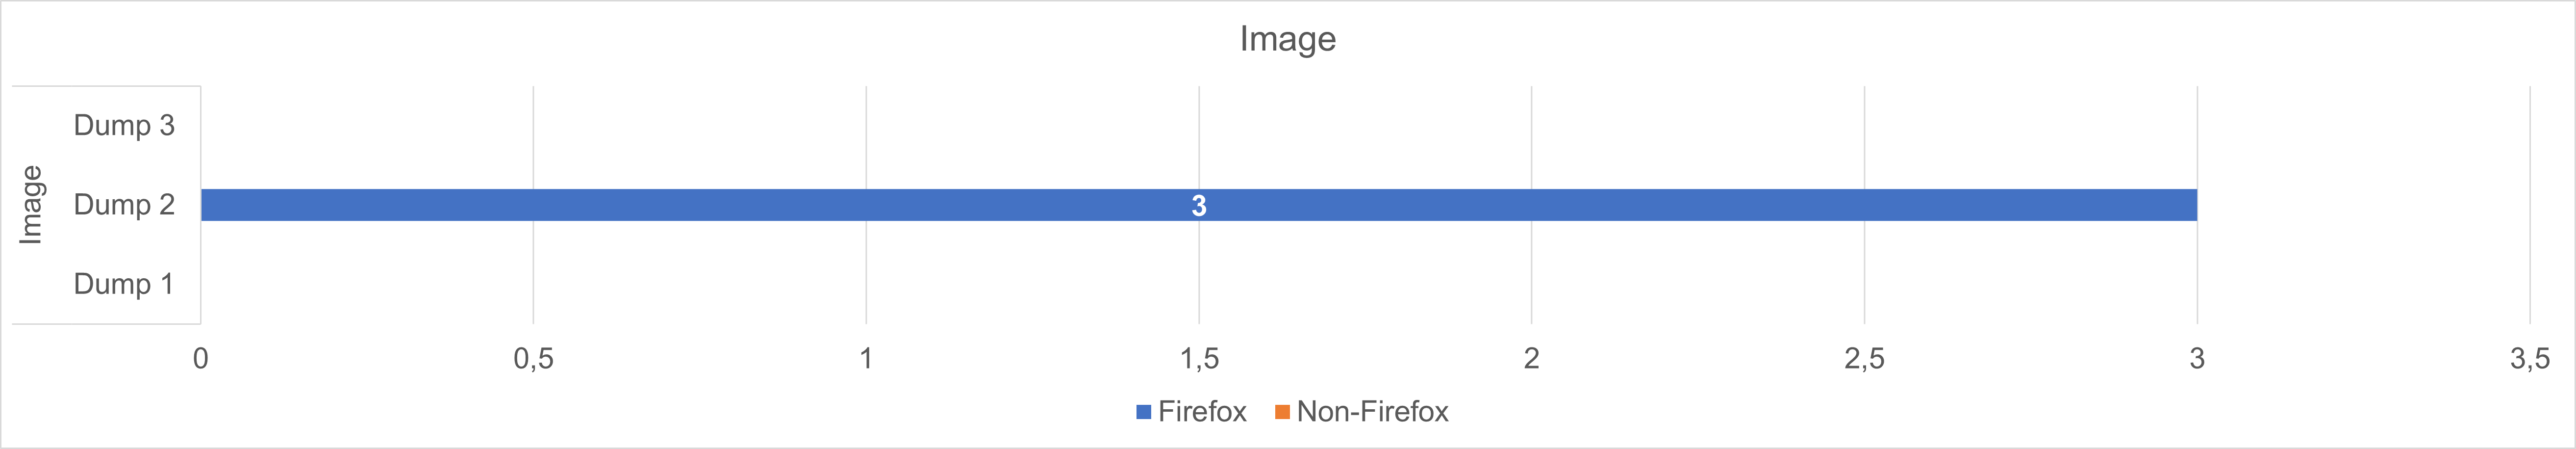
\includegraphics{bilder/volatility/firefox/image.png}}}
		\label{chart:final-criteria}  
		\caption{Image}
	\end{figure}
	Analyse:
		> Hex-Wert von Donaukurier Bild wurde im 2. RAM Dump in 3 Firefox Prozessen gefunden
	

Zusammenfassung = Stacked Bar Chart:
\begin{figure}[h!]
	\centerline{\resizebox{\linewidth}{!}{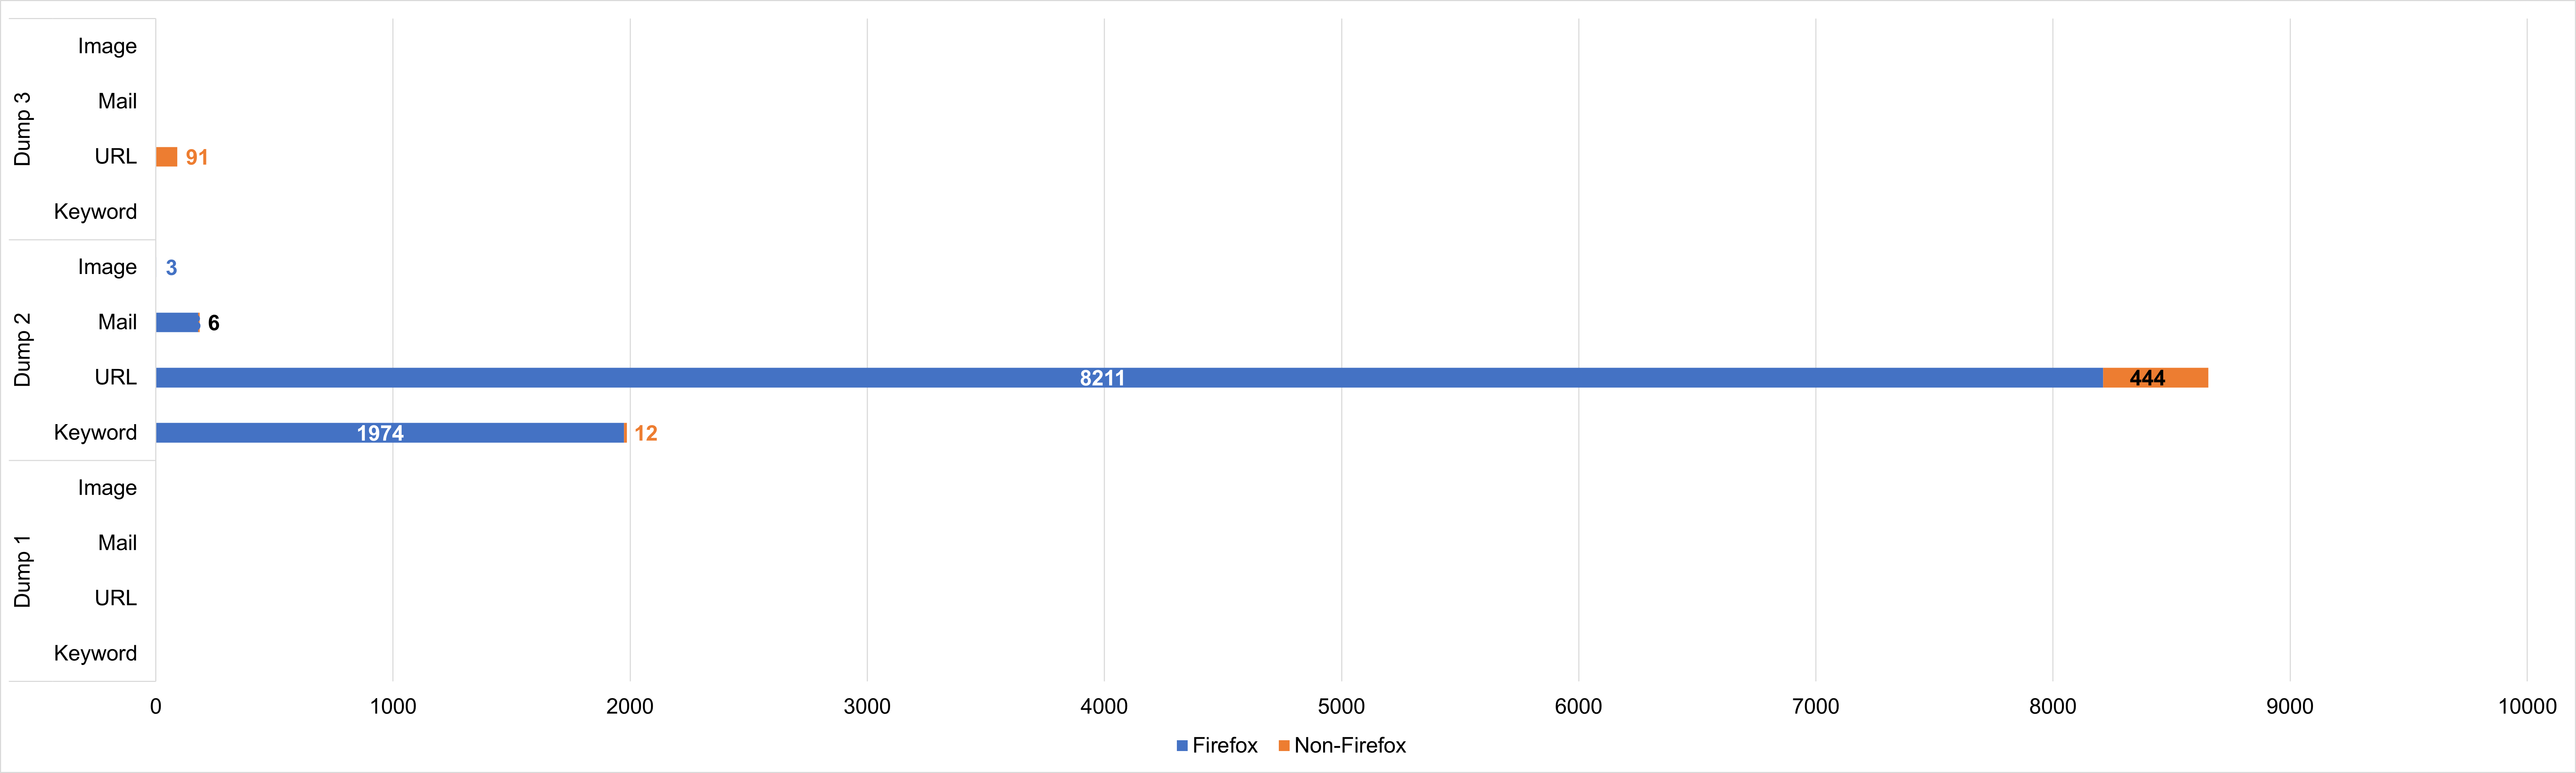
\includegraphics{bilder/volatility/firefox/summary.png}}}
	\label{chart:final-criteria}  
	\caption{Summary}
\end{figure}

TODO: Kreisdiagramme/Balkendiagramme mit Gesamtzahl an (Non-)Firefox Yarascan-Treffer erst im Vergleich mit Tor

\newpage


% ######################################################################
% ######################################################################
% ######################################################################
% ######################################################################


\section{Tor}

\subsection*{White-Box Analyse/Common Locations}

Schreiboperationen mit Process Monitor verfolgen:

Im Anhang: Tabelle mit allen geschriebenen Dateien (markiert, wenn nicht mehr wiederherstellbar + markiert, wenn Datei "verändert" (siehe oben: temp, WAL))

Aux-Dateien, welche nicht mehr vorhanden waren, aber dafür "richtige" Dateien:

Ergebnis: Tabelle mit wiederherstellbaren Dateien: Logfile 1 vs. Logfile 2 + Tool mit dem Datei untersucht wurde
- Dateien, die in beiden Logfiles nicht wiederherstellbar 
\begin{figure}[h!]
	\resizebox{\linewidth}{!}{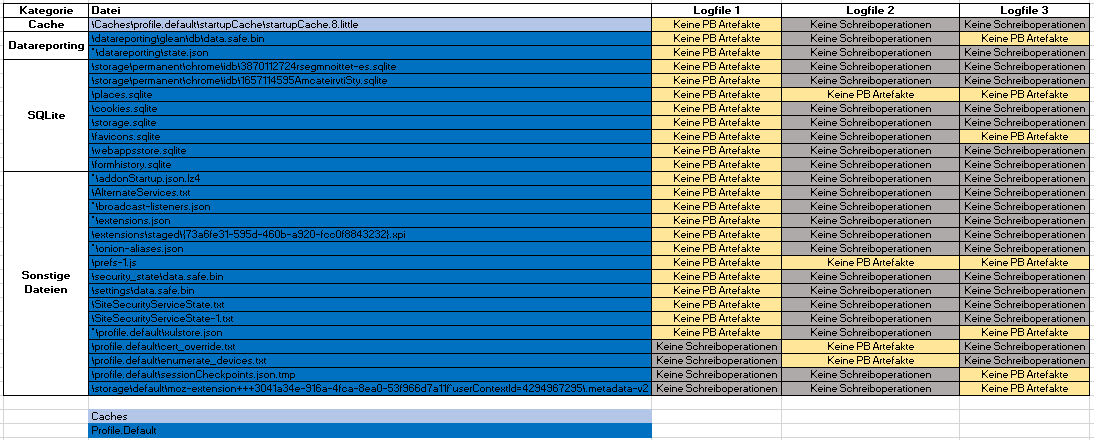
\includegraphics{bilder/tor-tabelle-logfile1vlogfile2vlogfile3-reduced.png}}
%	\label{...}
	\caption{Tabelle mit wiederherstellbaren Dateien: Logfile 1 vs. Logfile 2}
\end{figure}

Allgemein: Tor hat nur einen "Common Pfad"
-	% C:\Users\Forensik\Desktop\Tor Browser\Browser\TorBrowser\Data\Browser\
- Dateien tauchen in zwei unterschiedlichen Ordnern auf:
	- % C:\Users\Forensik\Desktop\Tor Browser\Browser\TorBrowser\Data\Browser\Caches\profile.default\ (Caches)
	- % C:\Users\Forensik\Desktop\Tor Browser\Browser\TorBrowser\Data\Browser\profile.default\ (Profile.Default)

- Alle Schreibopertationen von Prozess "firefox.exe" durchgeführt, nicht "tor.exe" 

=> Keine der Dateien enthält PB Artefakte, trotzdem nachfolgende genauere Betrachtung der wichtigsten Dateien im Zusammenhang des Tor Browsers

Kategorien der Logs:
- Cache: 
	> % \Caches\profile.default\startupCache\startupCache.8.little (Caches Folder)
	Zweck:
		"Die Datei "startupCache.8.little" ist eine interne Datei, die von Firefox und dem Tor Browser erstellt wird, um den Startvorgang des Browsers zu beschleunigen. Sie enthält im Wesentlichen eine Zwischenspeicherung von Daten, die beim Starten des Browsers benötigt werden.

		Diese Datei enthält Informationen über bereits geladene Browser-Komponenten wie JavaScript-Code, CSS-Dateien, Bilder und andere Ressourcen. Indem der Browser diese Informationen zwischenspeichert, kann er sie beim erneuten Starten des Browsers wiederverwenden, anstatt sie erneut herunterladen und verarbeiten zu müssen. Dadurch wird die Startzeit des Browsers verkürzt und die allgemeine Leistung verbessert." %https://wiki.mozilla.org/StartupCache
	Analyse:
		- Tool: HxD
		- kein PB Artefakte

- datareporting:
	> % *\datareporting\state.json 
	Zweck: 
		"Die Datei "state.json" im Ordner "/datareporting" enthält Informationen über den Zustand und die Konfiguration des Firefox- oder Tor Browsers. Diese Datei kann Daten über die Verwendung des Browsers, wie z.B. installierte Add-Ons, zuletzt besuchte Websites, Browser-Einstellungen und andere Informationen enthalten. Sie wird verwendet, um dem Browser bei Bedarf den Zustand und die Einstellungen wiederherzustellen."
		% https://github.com/mozilla/firefox-data-store-docs/blob/master/README.md
	Analyse:
		- Tool Notepad++ mit JSON Plugin
		- keine PB Artefakte

- Sonstige Dateien:
	> % \AlternateServices.txt
		Zweck:
			"enthält onion URLs,
			HTTP Alternative Services is a mechanism that allows servers to tell clients that the service they are accessing is available at another network location or over another protocol.
			This mapping can be stored in a file in the profile folder. This allows websites that do not support HTTPS to communicate in a secure way via port 443 (Opportunistic Encryption)."
			% https://support.mozilla.org/en-US/questions/1310302
	> % \extensions\staged\{73a6fe31-595d-460b-a920-fcc0f8843232}.xpi
		Zweck:
			"Ist "NoScript" Extension. Wenn in Firefox geöffnet, kann installiert werden"
		=> TODO: Screenshot, wenn in Firefox per "drag-and-drop" gezogen
	> % *\onion-aliases.json
		Zweck:
			Enthält SecureDrop Adressen: z.B. sueddeutsche.securedrop.tor.onion (z.B. %https://www.sueddeutsche.de/projekte/kontakt/#securedrop)
	> % \security_state\data.safe.bin
		Zweck: The file containing the updated security data % (https://bbs.archlinux.org/viewtopic.php?pid=1952286#p1952286)
	> % \SiteSecurityServiceState.txt
		Entielt früher private Browsing Artefakte (https://gitlab.torproject.org/tpo/applications/tor-browser/-/issues/18589), jetzt aber keine private Browsing Artefakte
	=> Keine der Dateien enthält PB Artefakte
				
- SQLite: 
	Aus Process Monitor Logfiles erkennbar: Tor verwaltet und beschreibt die exakt gleichen SQLite Datenbanken wie Firefox.

	Hier ebenfalls gesondert betrachtet: Fokus auf die Entwicklung von Dateiinhalt in allen Snapshots (1, 2, 3-1, 3 und 4) betrachtet
	
	Ergebnisse:
		\begin{figure}[h!]
			\centerline{\resizebox{\linewidth}{!}{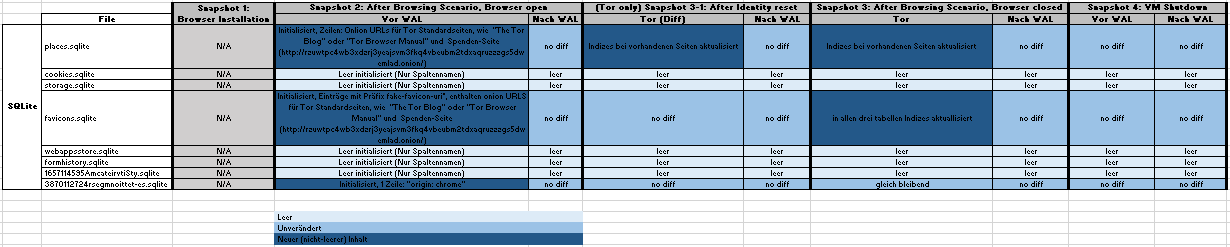
\includegraphics{bilder/tor-sqlite-table.png}}}
			\label{chart:final-criteria}  
			\caption{Comparison of found PB artifacts between RAM Dumps}
		\end{figure}
		> Nach Browser-Installation noch keine SQLite-Datei angelegt (Snapshot 1)
		> Während Browsing Szenario alle DBs Initialisiert, außer "webappsstore.sqlite" (Snapshot 2)
			- Dabei wurden in places.sqlite automatisch .onion URLs geschreiben, die zu Tor Standardseiten führen, wie "The Tor Blog" oder "Tor Browser Manual" bzw. die Tor Spenden-Seite, obwohl keine dieser Seiten aufgerufen wurde
				TODO: Screenshot von URLs?
			- in Favicons.sqlite wurden die exakt gleichen Enträge geschrieben, mit dem Präfix "Fake-favicon-uri". Ein tatsächliches Icon wurde nicht in die DB geschrieben
			- remote settings Datenbank enthielt den gleichen Eintrag wie es bereits bei Firefox der Fall war. Keine PB Artefakte
			- Restliche Dateien ohne Inhalt, nur Spaltennamen
			- Nach WAL Checkpoints bleiben Dateien unverändert
		> Nach Zurücksetzen der Browser-Identität (Snapshot 3-1)
			- in places.sqlite: Indizes bei eingetragenen Seiten aktualisiert
			- restliche Dateien unverändert
		> Nach Schließen des Browsers (Snapshot 3)
			- in places.sqlite sowie favicons.sqlite: Indizes bei eingetragenen Seiten aktualisiert
			- restliche Dateien unverändert
			- nach WAL Checkpoints bleiben Dateien unverändert
		> Nach herunterfahren der VM (Snapshot 4)
			- Alle Dateien unverändert, auch nach WAL Checkpoint
	
- Zusammenfassung: in keiner Datei PB Artefakte


Quantitativ: (Diagramme)		
	> Balkendiagramm: Für jede Logfilekategorie: Anzahl Schreiboperationen Logfile 1 vs Logfile 2
	\begin{figure}[h!]
		\centerline{\resizebox{\linewidth}{!}{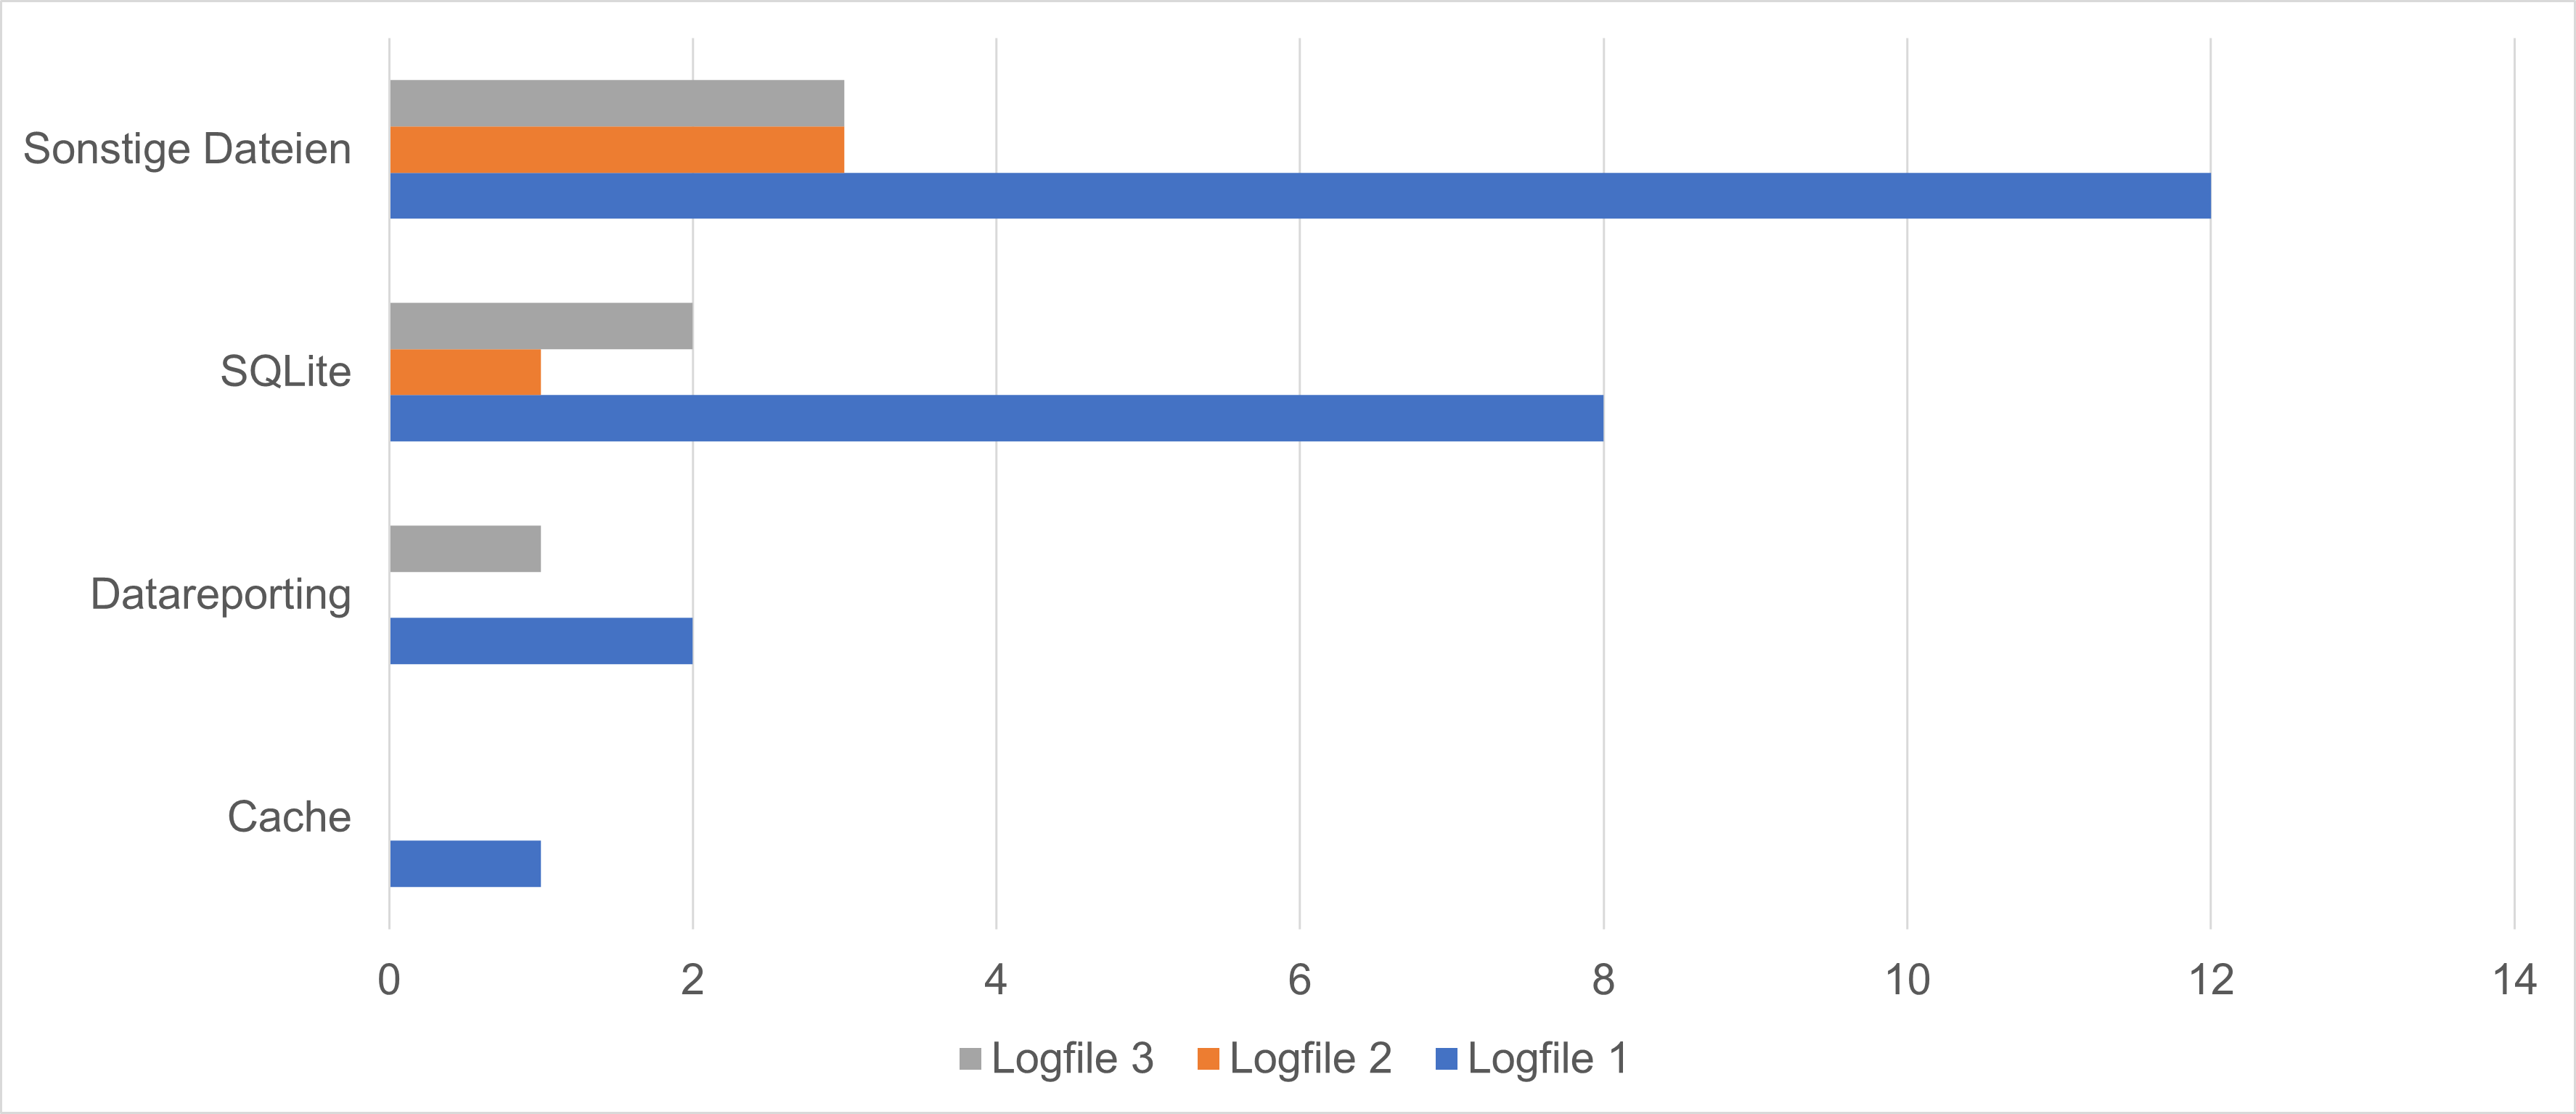
\includegraphics{bilder/tor-bar-chart-logfile1vs2cs3.png}}}
		\label{chart:final-criteria}  
		\caption{Comparison of found PB artifacts between RAM Dumps}
	\end{figure}

%Literatur:
%	o no traces were found in “common locations” \cite{Montasari.2015}
%		>  “places.sqlite”, “webappsstore. sqlite”, “sessionstore.bak”, “search.json” and “nssckbi.dll”
%	o	Safebrowsing: Alle Dateien in /safebrowsing-updating/ nicht relevant. Dort nur .vlpset und .sbstore Dateien. Speichern 256-Bit Hash von URLs, die auf SafeSearch Blacklist stehen 
%	o	Cache-Dateien: drei Caches: startupCache, jumpListCache (beide enthalten Binärdateien ohne Browsing Artefakte) und cache2 (können mit MozillaCacheView untersucht werden, enthalten keine Browsing Artefakte)
%	o	SQLite Datenbanken: Sqlite Dateien erst ohne WAL Dateien untersuchen, Danach mit sqlite3 Konsole: WAL in Datenbank schreiben mit: PRAGMA wal\_checkpoint; places.sqlite besonders relevant, da dort Browser in public Modus Browsing URLs verwaltet (Am besten hier vergleich mit Public Browsing machen)	
%		> \cite{Fayyad.2021} for Mozilla Firefox, 7 database files were recovered: cookies.sqlite-shm, places.sqlite-shm, prefs.js etc.
%		> \cite{Muir.2019} The two SQLite databases used by Firefox to track cookies and history (cookies.sqlite und places.sqlite) were both recoverable from the file system after deletion	
%		Ergebnisse stehen im Gegensatz zu \cite{Hedberg.2013} :
%			o	Chrome und Firefox: Einträge in places.sqlite + history.sqlite DB gefunden während PB! (Noch aktuell??)
%		Sonderfall: SQlite DB-Crash \cite{Hedberg.2013}
%			> WAL Files/Journal Files bei Crash gefunden -> Kann genutzt werden um zu beweisen, dass privater Browser genutzt wurde
%			> Daher: WAL Rollback mit sqlite3	
%	o	Jsonlz4 \& balkz4: Enthalten komprimierte Firefox-Sessions, jsonlz4 Dateien können mit Tool "entkomprimiert" werden: https://www.jeffersonscher.com/ffu/scrounger.html


\subsection*{Registry}
> Process Monitor: SetValue Operationen von Browser 
	Kategorien Registry Keys: Analog zu Firefox
	1) PreXULSkeletonUISettings:
		> Prefix: Absoluter Installationspfad von Firefox
		> Skeleton UI Einstellungen von Firefox % https://itigic.com/skeleton-ui-new-firefox-interface-to-start-up-much-faster/#google_vignette
			Definition:
				> Der "PreXULSkeletonUISettings" Registry Key enthielt Einstellungen für die Benutzeroberfläche (UI) des Firefox-Browsers, insbesondere für das sogenannte "Skeleton UI". Das Skeleton UI ist eine vereinfachte Benutzeroberfläche, die während des Ladens des Browsers angezeigt wird, bevor die vollständige Benutzeroberfläche geladen ist. Es besteht aus grundlegenden Steuerelementen und Elementen, die dem Benutzer die Interaktion ermöglichen, während der Rest der Benutzeroberfläche noch geladen wird.
				> Der "PreXULSkeletonUISettings"-Schlüssel enthielt Konfigurationsoptionen wie Farben, Positionen und andere Einstellungen für das Skeleton UI. Durch das Bearbeiten dieses Schlüssels konnten Benutzer die Darstellung des Skeleton UI anpassen. Es ist jedoch wichtig zu beachten, dass das Ändern der Registrierungseinträge ein fortgeschrittenes Verfahren ist und Fehler zu Problemen mit dem Browser führen kann.
			
		> Struktur der Keys: % HKCU\SOFTWARE\Mozilla\Firefox\PreXULSkeletonUISettings\C:\Program Files\Mozilla Firefox\firefox.exe|<UI Einstellung>
		> Unterschiedliche UI Einstellungen
			- % ScreenX (DWORD)
			- % ScreenY (DWORD)
			- % Width (DWORD)
			- % Height (DWORD)
			- % Maximized (DWORD)
			- % Flags (DWORD)
			- % CssToDevPixelScaling (REG_BINARY)
			- % UrlbarCSSSpan (REG_BINARY)
			- % SearchbarCSSSpan (REG_BINARY)
			- % SpringsCSSSpan (REG_BINARY)
		> keine PB Artefakte unter UI Einstellungen	
	2) Business Activity Monitoring % https://learn.microsoft.com/de-de/biztalk/core/business-activity-monitoring-bam
		> Quelle: % https://notes.qazeer.io/dfir/windows/_artefacts_overview
		> BAM is a mostly undocumented feature that controls the programs executed in the background. DAM is a feature for devices supporting the "Connected Standby" mode (i.e when a device is turned on, but its display will be turned off). As a result, the BAM registry keys will contain data on any devices, while DAM registry keys will only contain data on mobile devices.
		> The BAM registry key contains multiple subkeys under bam\\State\\UserSettings, with one subkey per user, identified with the user SID. While the key is in the SYSTEM registry hive, program executions can thus still be tied to a specific user using this SID.
		> Each user-specific key contains a list of executed programs, with their full path and timestamp of last execution.
		> If a file is deleted, the eventual associated entry in the BAM is deleted as well after the system reboot. Additionally, BAM entries older than 7 days are deleted upon system boot. The BAM thus provides limited information on historic execution of programs
		> No entries are created in the BAM keys for executables on removable media and/or on network shares.
		> Key: %  HKLM\System\CurrentControlSet\Services\bam\State\UserSettings\S-1-5-21-588412547-2749917301-3803556669-1001\\Device\HarddiskVolume2\Program Files\Mozilla Firefox\firefox.exe (REG_BINARY)

Quantitativ: (Diagramme)
	- Stacked Balkendiagramm jeweils für Logfile 1 und Logfile2: Anteil Kategorie 1 bzw.2 an allen Registry-Schreiboperationen
	\begin{figure}[h!]
		\centerline{\resizebox{\linewidth}{!}{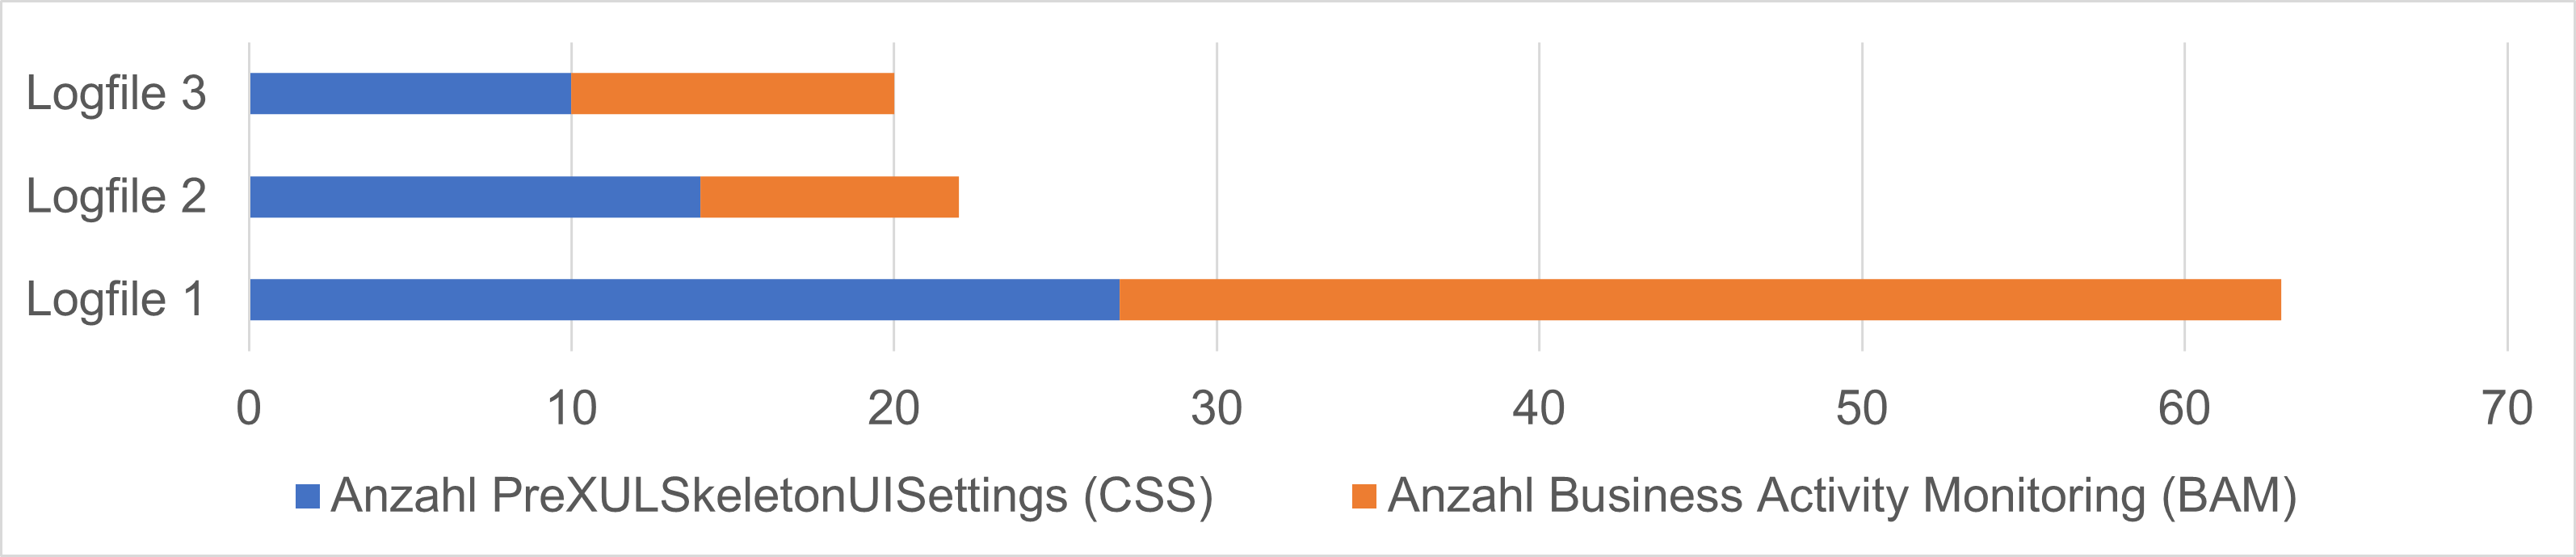
\includegraphics{bilder/tor-registry-stacked-bar-chart.png}}}
		\label{chart:final-criteria}  
		\caption{Comparison of found PB artifacts between RAM Dumps}
	\end{figure}
	
> Stringsuche in Registry Hives mit Registry Explorer (Siehe Liste)
	In allen Hives kein Treffer für alle Suchbegriffe

Literatur: 
	> Wie bei Firefox: Shellactivities Key existiert nicht mehr --> Nicht mehr vorhanden in aktueller Version (Verweis auf E-Mail)

%Literatur:
%	>	Auf Autor verweisen: angeblich in Shellactivities Ergebnisse. --> Nicht mehr vorhanden in aktueller Version (Verweis auf E-Mail)
%	>	Process Monitor/Regshot zeigen keine relevanten Key-Änderungen
%	> \cite{Muir.2019}: Autopsy Keyword Suche nach Suchbegriffen: Ergebnisse in \%SystemRoot\%Minidump NTUSER.DAT, ntuser.dat.LOG1 (a log of changes to NTUSER.DAT)
%	> Zentral: shellactivites Key:	NTUSER.DAT --> “shellactivities” key \cite{Muir.2019}
%	> \cite{Rochmadi.2017} Detection of registry changes helps to determine what the appropriate plugin is used to search for digital evidence using volatility memory forensic:
%	- RegQueryValue:	HKCU/Software/Microsoft/Windows/CurrentVersion/InternetSettings/Connections/DefaultConnectionSettings
%	- RegCloseValue: 	HKCU/Software/Microsoft/Windows/CurrentVersion/InternetSettings/Connections
%	- IRP\_MJ\_READ: C:/pagefile.sys

\subsection*{Black-Box Analyse/Uncommon Locations}

\subsubsection*{Analyse mit Autopsy}
Bei White-Box Analyse/Common Locations: Autopsy nur zur Dateiextraktion genutzt, hier: als konkretes forensisches Werkzeug

Stichwortsuche:
- In allen Snapshots keine Treffer (auch innerhalb \$Carved)
- TODO: Pagefile gefunden?

Von Autopsy automatisch indexierte Dateien: 
In allen Fällen: keine Dateien gelöscht, nur über Zeitraum der Snapshots neue dazugekommen
- Web Bookmarks:
	\begin{figure}[h!]
		\centerline{\resizebox{\linewidth}{!}{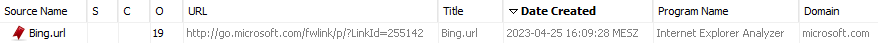
\includegraphics{bilder/cfv_tor_autopsy_web_bookmarks.png}}}
		\label{chart:final-criteria}  
		\caption{Autopsy Web Bookmarks}
	\end{figure}
	Snapshot 1:
		> Bing.url (Unter C:/User/Forensik/Favorites/Links) enthält Bing Startseite
	Snapshot 2:
		> unverändert zu 1
	Snapshot 3-1:
		> unverändert zu 2
	Snapshot 3-2:	
		> unverändert zu 3-1
	Snapshot 4:
		> unverändert zu 3-2
- Web Cookies:
	\begin{figure}[h!]
		\centerline{\resizebox{\linewidth}{!}{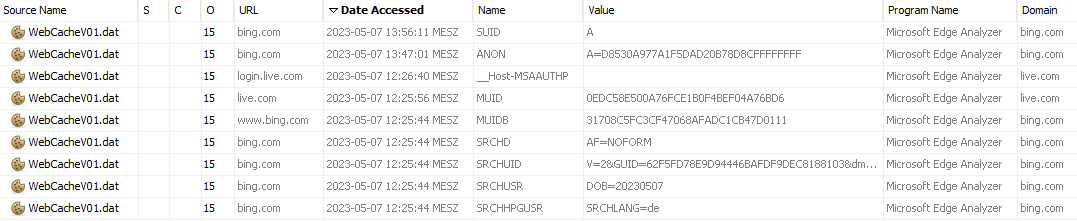
\includegraphics{bilder/cfv_tor_autopsy_web_cookies.png}}}
		\label{chart:final-criteria}  
		\caption{Autopsy Web Cookies}
	\end{figure}
	Snapshot 1:
		> 9 Einträge in WebCacheV01.dat (= DB des Internet Explorers zum speichern von Browserdaten): Cookies für bing.com und live.com (= outlook)
	Snapshot 2:
		> unverändert zu 1
	Snapshot 3-1:
		> unverändert zu 2
	Snapshot 3-2:
		> unverändert zu 3-1
	Snapshot 4:
		> unverändert zu 3-2
- Web History:
	\begin{figure}[h!]
		\centerline{\resizebox{\linewidth}{!}{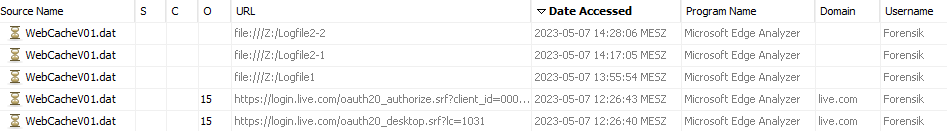
\includegraphics{bilder/cfv_tor_autopsy_web_history.png}}}
		\label{chart:final-criteria}  
		\caption{Autopsy Web History}
	\end{figure}
	Snapshot 1:
		> 2 Einträge in WebCacheV01.dat:
			- 2x live.com (= outlook)
	Snapshot 2:
		> 1 neuer Einträge in WebCacheV01.dat:
			- file:///Z:/Logfile\_1 (= Process Monitor Logfile, die in shared-Folder geladen wurde) -> Erklärung?
	Snapshot 3-1:
		> 1 neuer Eintrag in WebCacheV01.dat:
			- file:///Z:/Logfile\_2-1 (= Process Monitor Logfile, die in shared-Folder geladen wurde) -> Erklärung?
	Snapshot 3-2:
		> 1 neuer Eintrag in WebCacheV01.dat:
			- file:///Z:/Logfile\_2-2 (= Process Monitor Logfile, die in shared-Folder geladen wurde) -> Erklärung?
	Snapshot 4:
		> unverändert zu 3-2
- Web Categories:
	\begin{figure}[h!]
		\centerline{\resizebox{\linewidth}{!}{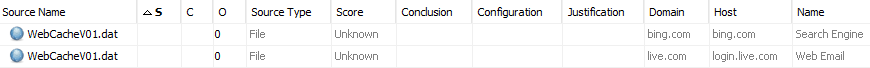
\includegraphics{bilder/cfv_tor_autopsy_web_categories.png}}}
		\label{chart:final-criteria}  
		\caption{Autopsy Web Categories}
	\end{figure}
	Snapshot 1:
		> 2x WebCacheV01.dat aufgelistet => Mit HxD untersucht, keine PB Artefakte
	Snapshot 2:
		> unverändert zu 2
	Snapshot 3-1:
		> unverändert zu 3
	Snapshot 3-2:
		> unverändert zu 3-1
	Snapshot 4:
		> unverändert zu 3-2
		
Zusammenfassung:
- keine PB Artefakte
- Keine neuen Erkenntnisse vgl. mit intensiver Analyse mittels Process Monitor in Kapitel X
- .onion URL Einträge in places.sql nicht erkannt

%Literatur:
%	o	Autopsy Keywortsuche: 
%		>	In alles Snapshots ergebnislos (keine Keyword-Hits
%		-->	In Literatur: Autoren fanden Ergebnisse in pagefile.sys 
%			> Autopsy: websites and some of the keywords found in hidden file called “pagefile.sys” \cite{Mahlous.2020}
%			o \cite{Montasari.2015} traces were found in: 
%				> However, on investigating the “pagefile.sys”, some entries were discovered
%				> Using the “data carving” technique, profile picture was recovered
%			o \cite{Said.2011} 
%				> Examining pagefile.sys showed some positive hits 			
%		--> Evtl. hier zeigen, was gefunden werden kann, wenn RAM reduziert
%		--> Aber auf Problem hinweisen, dass gefundener String in pagefile nicht direkt Browser zugeordnet werden kann
%		> \cite{Gabet.2018}	Firefox only produced three recoverable artefacts as reported by both tools (FTK, Autopsy) --> Artefakte werden nicht genannt!
%		> \cite{Muir.2019} Autopsy Keyword Suche nach Suchbegriffen: unallocated space
%		> Autopsy Carving Module (\$Carved): \cite{Muir.2019}
%			•	When searching for the string ’clot’ from the browsing protocol, six .dll, .edb and .reg files were discovered in unallocated space.
%			•	Further searching of unallocated space uncovered references to the Tor installation directory and the obfs4 bridging IP addresses
%			•	browsing data found in NTUSER.DAT was also replicated in unallocated space.
%	o	Autopsy PlugIns:
%		>	*** TODO: Hier Liste mit PlugIns ***

\subsubsection*{Analyse mit Volatility}
Vorgehen: Siehe "Methodik" Kapitel
	- Ausgangslage: Volatility Yarascan Treffer
	- Für jeden Treffer: virtueller Offset des Strings, PID, getriggerte Yararule, getriggerte Yara Component z(= Variablenname des gesuchten Strings), gefundener String
	- Neue Spalte: "Prozessname" -> zu jeder PID Prozessnamen
	- Ergebnisse Aufbereitet nach folgendem Schema:
		> Für jeden RAM Dump
		> Für jede Yararule
		> Für jede Component
		> Filter: Prozessname = Firefox -> Anzahl zählen
		> Filter: Prozessname = Alle Prozesse außer Firefox -> Anzahl zählen

Wie bei Firefox: HTML Artefakte wurden in keinem RAM Dump gefunden => Nicht aufgeführt

Yararule "Keyword":
	\begin{figure}[h!]
		\centerline{\resizebox{\linewidth}{!}{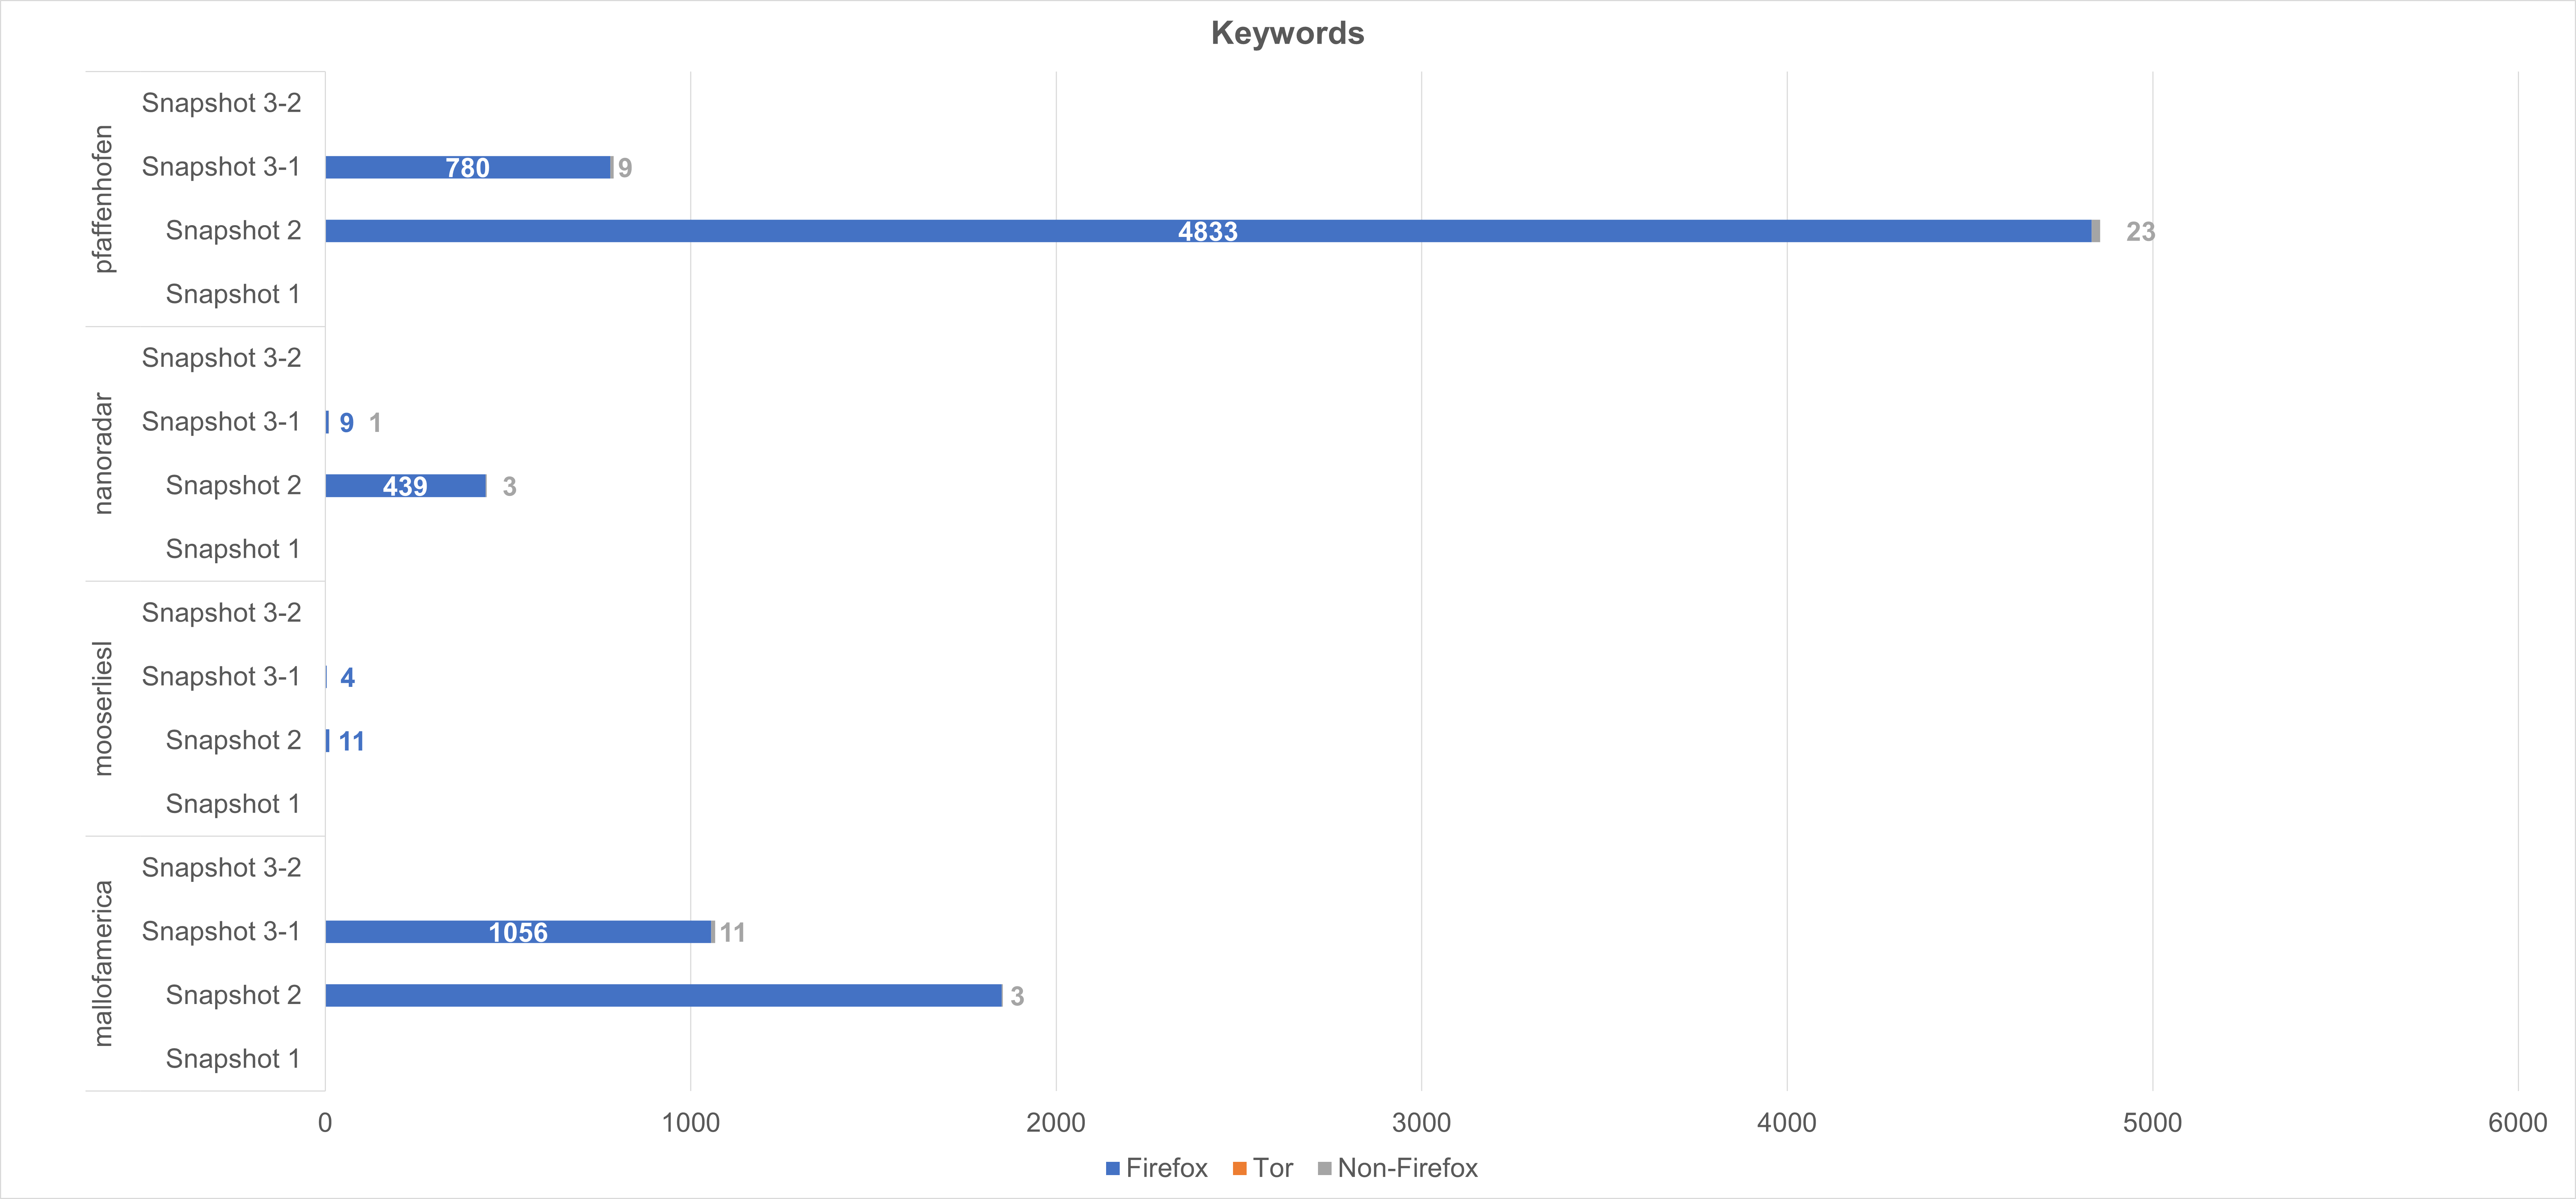
\includegraphics{bilder/volatility/tor/keywords.png}}}
		\label{chart:final-criteria}  
		\caption{Keywords}
	\end{figure}
	Analyse:
		> Ausschließlich in RAM Dump 2 und RAM Dump 3-1 Keyword Artefakte gefunden
		> In RAM Dump 3-1 bei jedem Keyword deutlich weniger Artefakte als in RAM Dump 2 => Identitäts-Reset reduziert Keyword Artefakte deutlich
		> Hauptsächlich in Firefox Prozess, kein Artefakt in Tor.exe Prozess
		> Mit 4833 Artefakten in RAM Dump 2 am häufigsten "pfaffenhofen" vertreten. Vermutung: Evtl. weil Google Maps viele zusätzliche Artefakte lädt. 
		> Nach Schließen von Tor Browser: keine Keyword Artefakte mehr in RAM
		
Yararule "URL":
	\begin{figure}[h!]
		\centerline{\resizebox{\linewidth}{!}{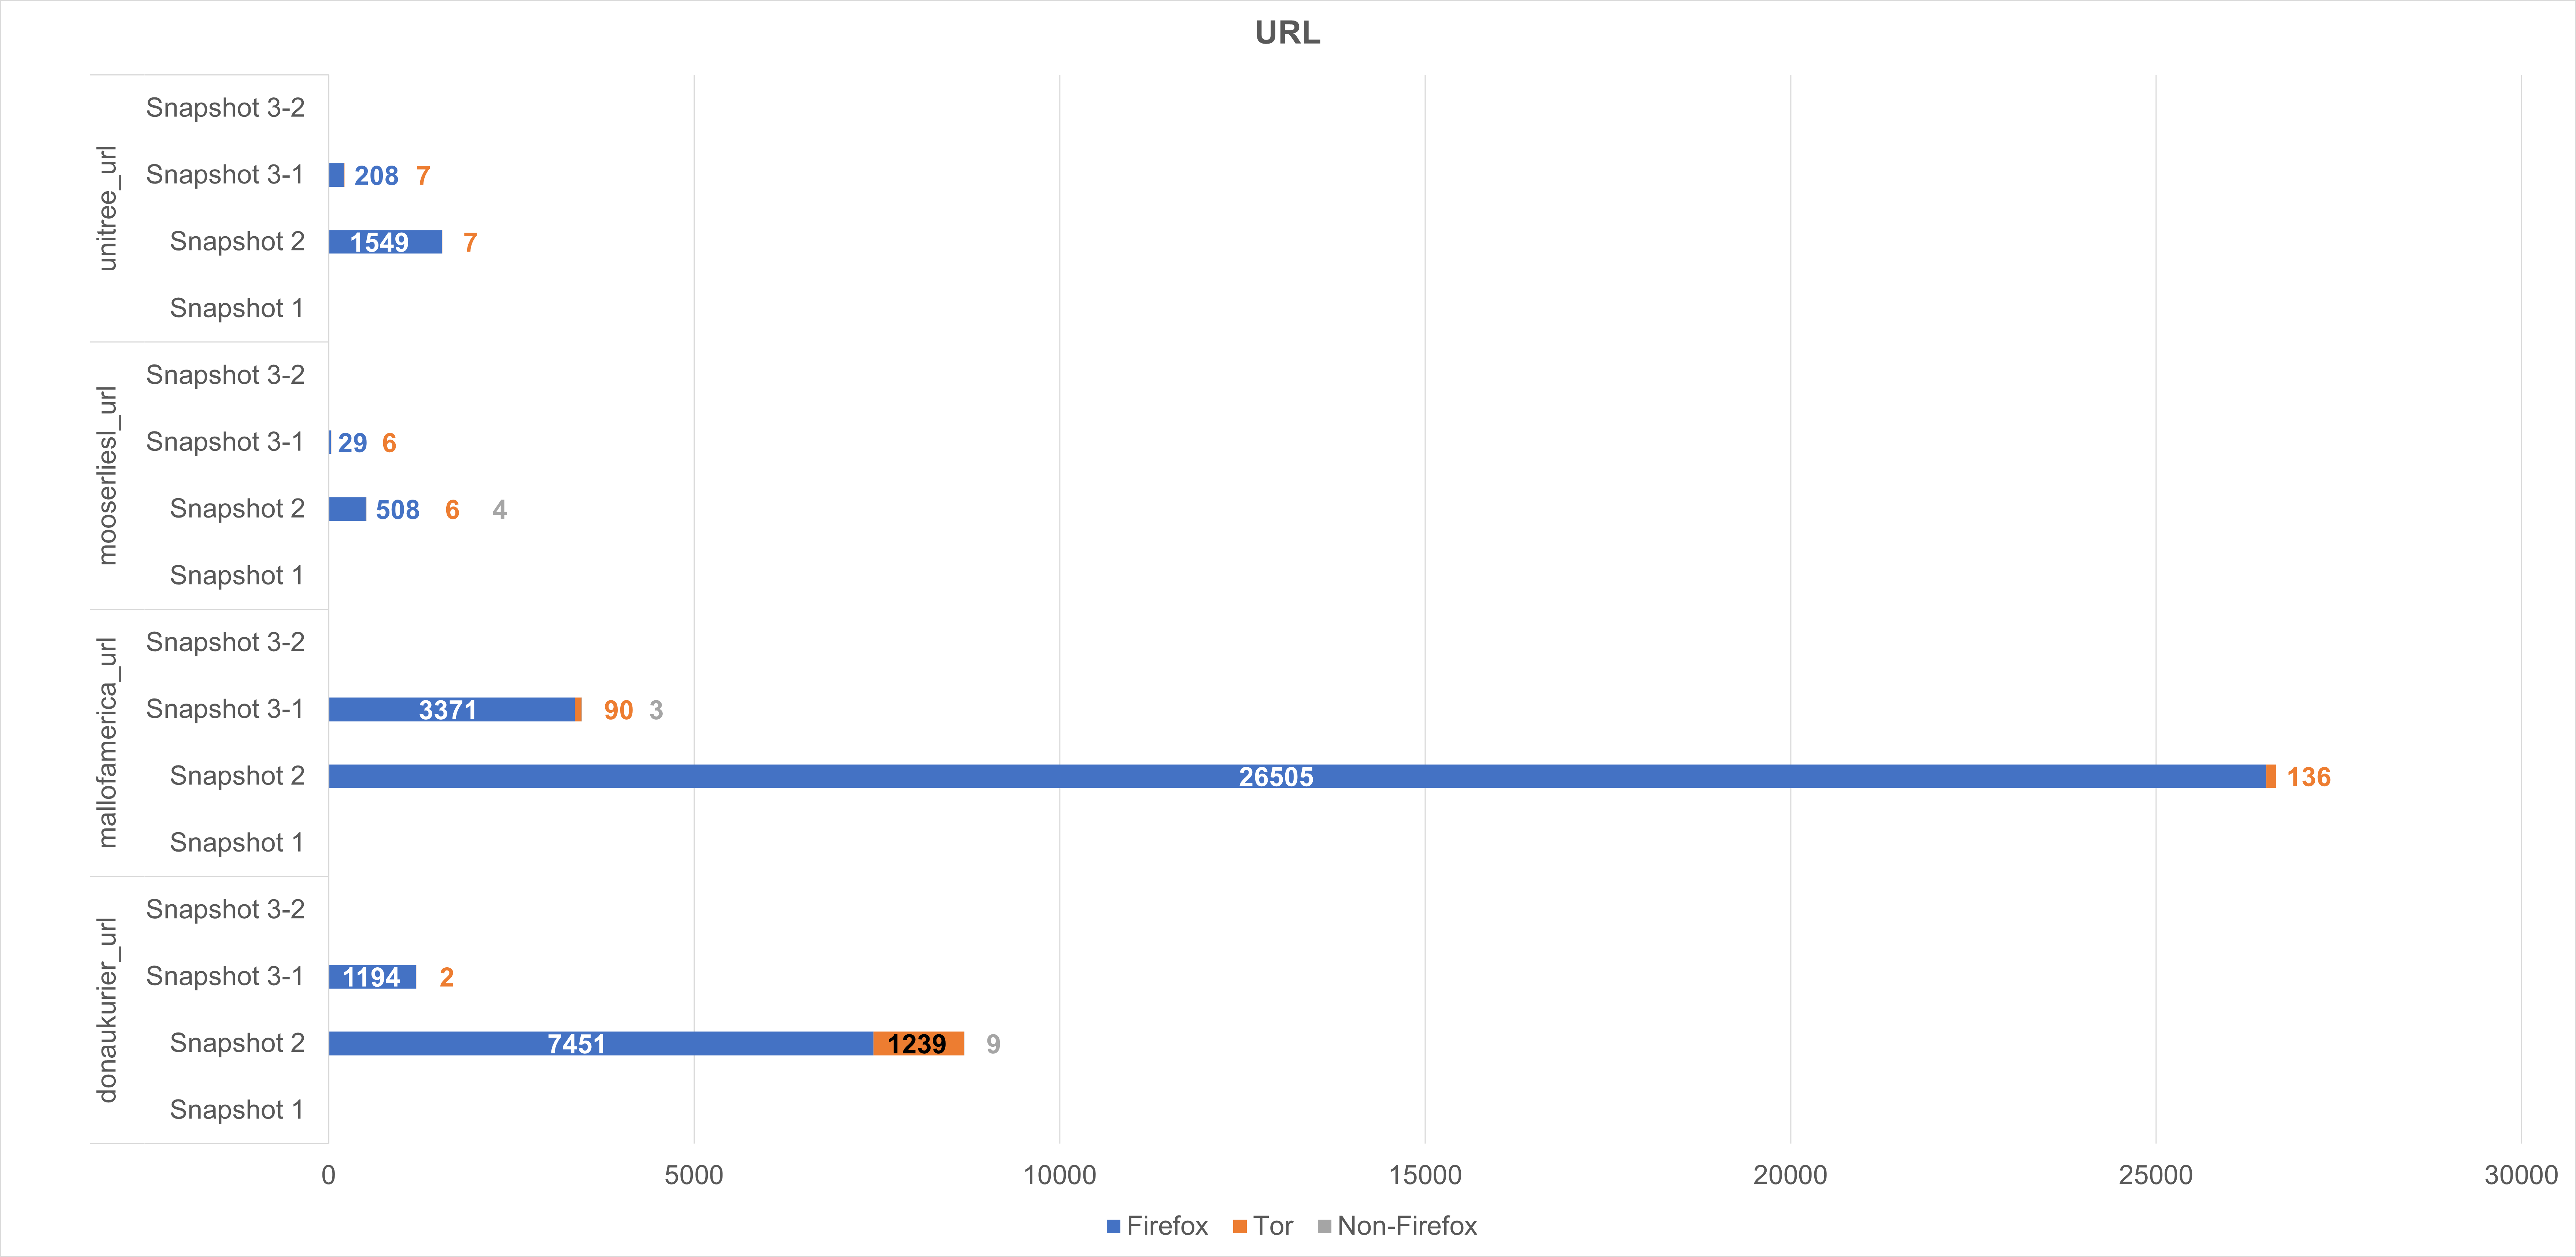
\includegraphics{bilder/volatility/tor/url.png}}}
		\label{chart:final-criteria}  
		\caption{URL}
	\end{figure}
	Analyse:
		> Wie bei Yararule "Keyword": Ausschließlich in RAM Dump 2 und RAM Dump 3-1 Keyword Artefakte gefunden
		> In RAM Dump 3-1 bei jedem Keyword deutlich weniger Artefakte als in RAM Dump 2 => Identitäts-Reset reduziert URL Artefakte deutlich
		> Hauptsächlich in Firefox Prozess, danach am häufigsten Tor.exe Prozess und am wenigsten Artefakte in anderen Prozessen
		> Bemerkenswert: "mallofamerica.com" ist mit 26.505 mal in RAM Dump 2 am häufigsten als Artefakt gefunden worden. Vergleich: "mooserliesl.de" wurde nur 508 mal in RAM Dump 2 gefunden
		> Nach Schließen von Tor Browser: keine URL Artefakte mehr in RAM
		
		> TODO: DNSCache?

Yararule "Mail":
	\begin{figure}[h!]
		\centerline{\resizebox{\linewidth}{!}{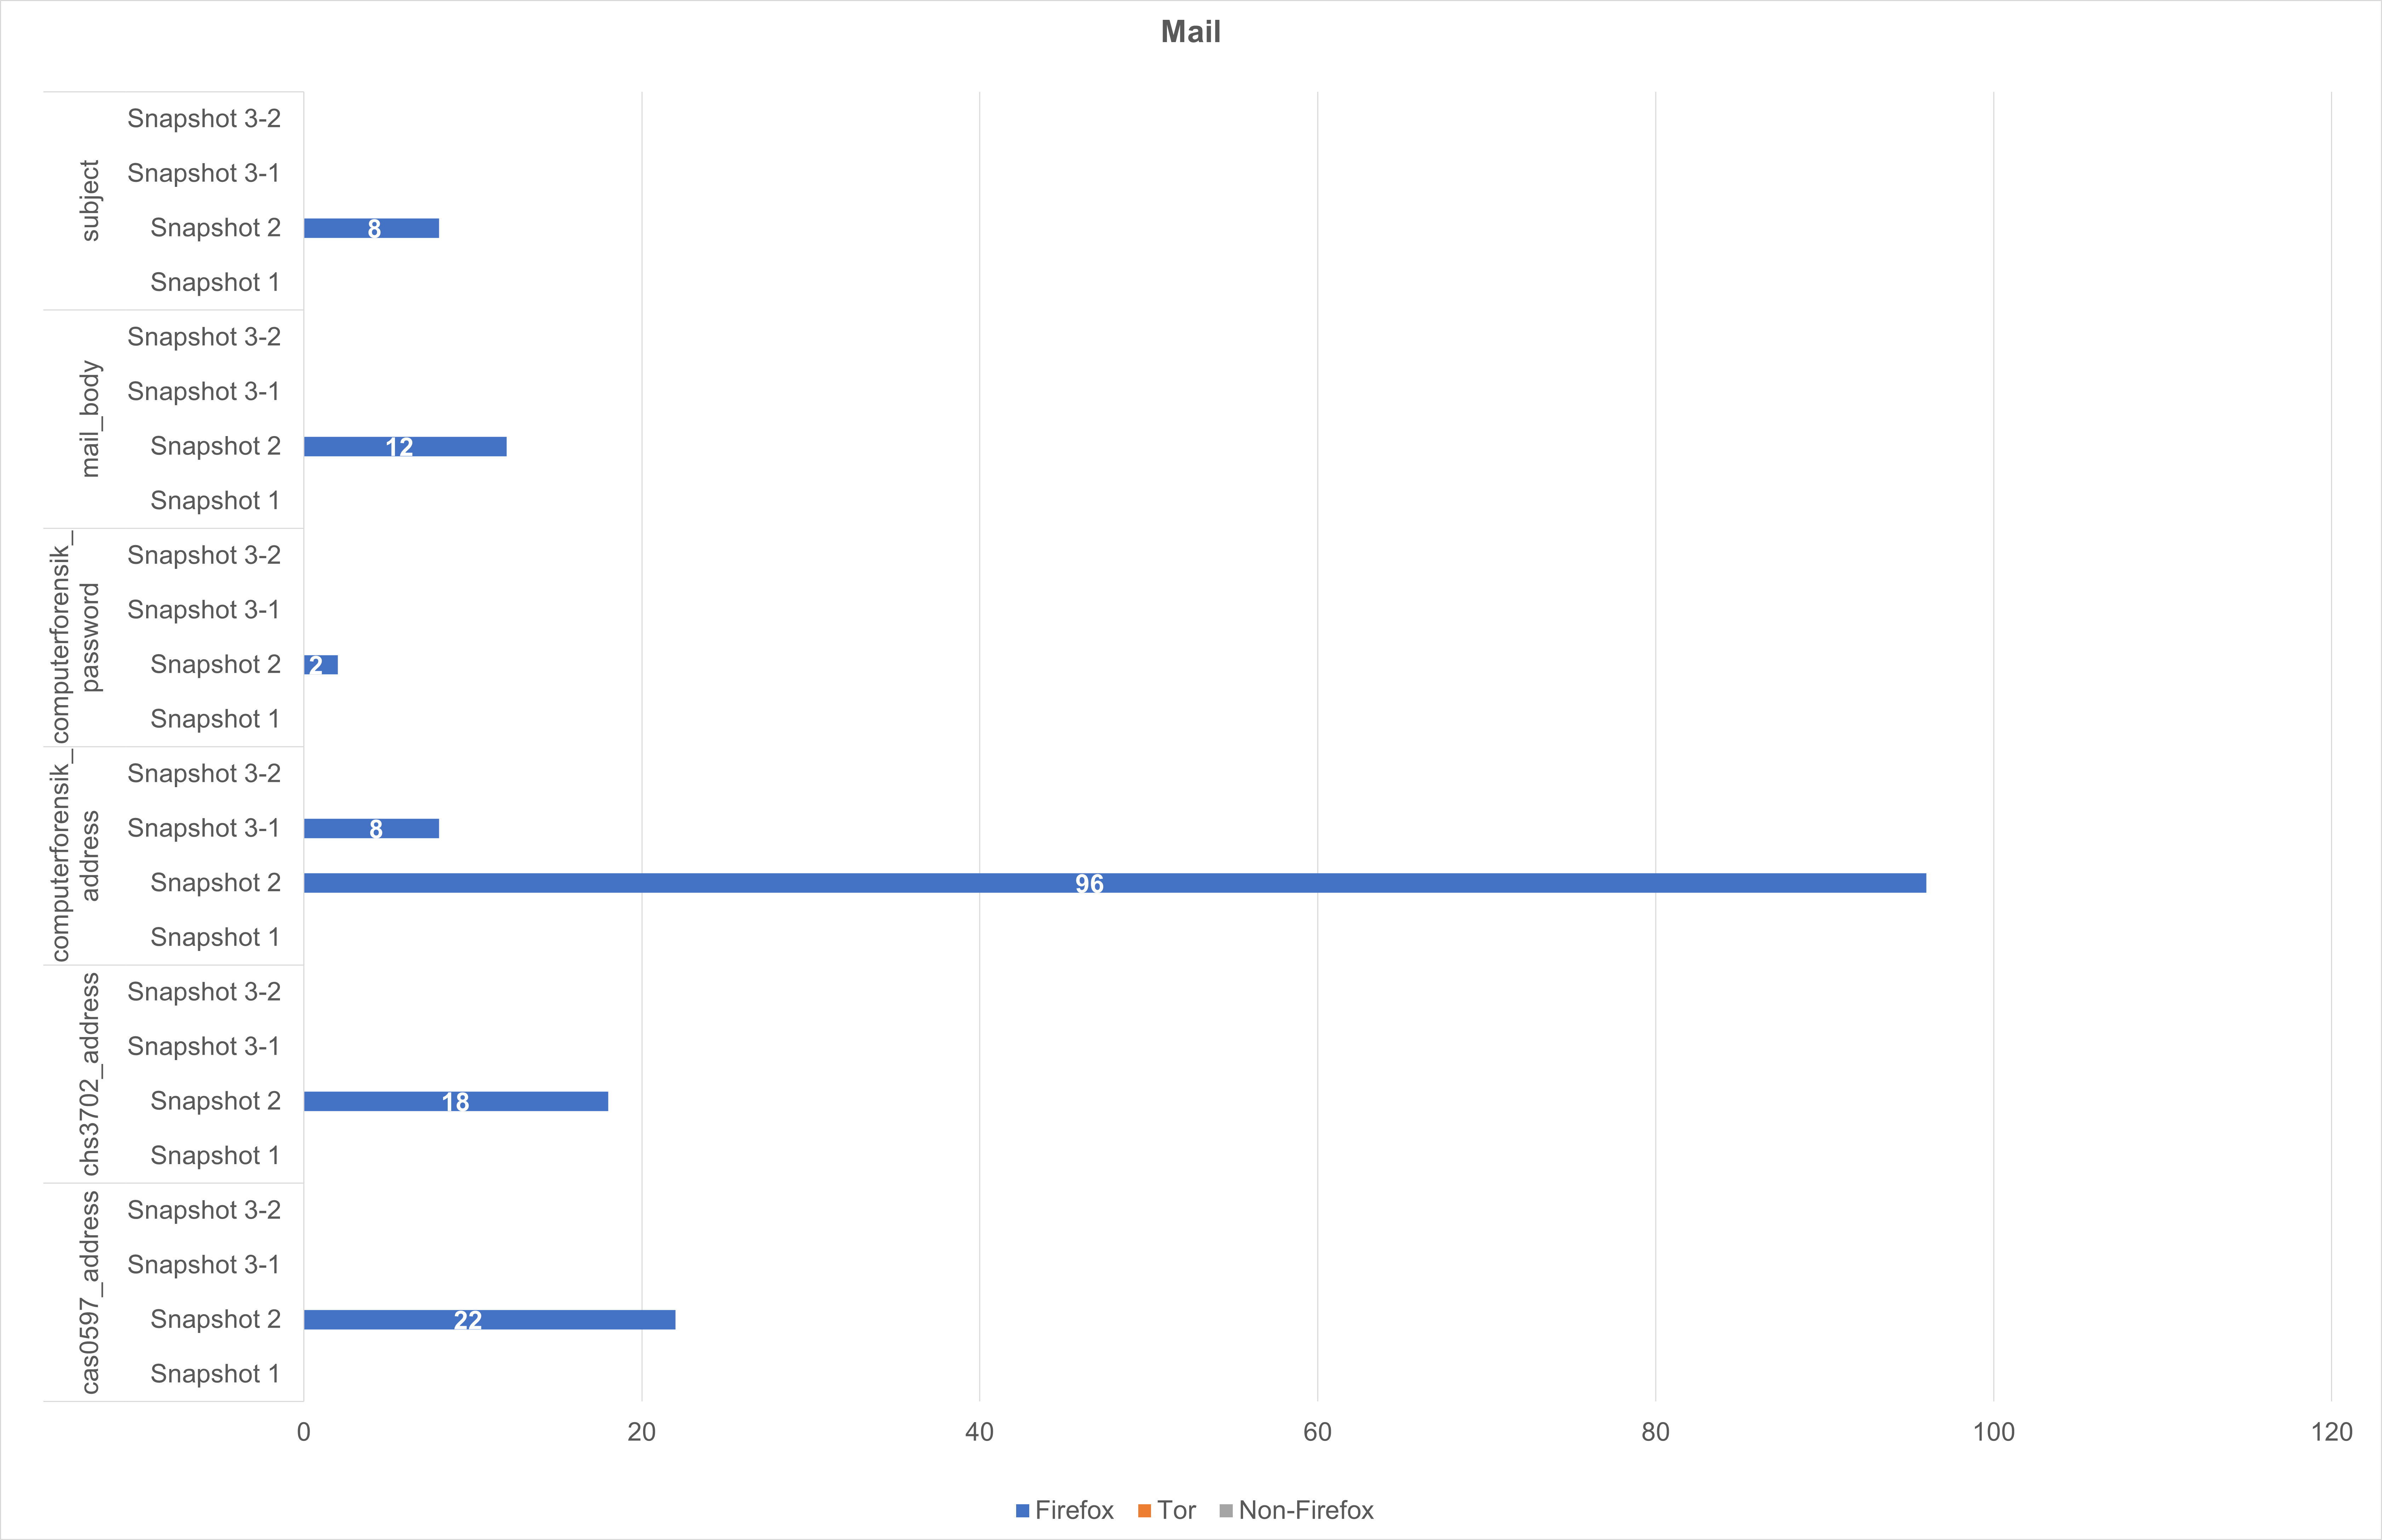
\includegraphics{bilder/volatility/tor/mail.png}}}
		\label{chart:final-criteria}  
		\caption{Mail}
	\end{figure}
	Analyse:
		> Alle Mail Artefakte gefunden
		> Artefakte ausschließlich in Firefox Prozess gefunden
		> Artefakte fast ausschließlich in RAM Dump 2 Mail gefunden
		> Nur die Absenderadresse "computerforensikvl@gmail.com" wurde nach Identitäts-Reset in RAM Dump 3-1 gefunden
		> Absenderadresse ist häufigstes Mail Artefakt
		> Bemerkenswert: Passwort wurde 2x als Klartext im RAM gefunden!
			String Kontext:
				Offsets:		PIDs:
				0xb9ce29180c8	7420
				0x2859f4ffd4e0	7420
				0x24083b41858	8424
				0x240840e5b08	8424
				
Yararule "Image":
	\begin{figure}[h!]
		\centerline{\resizebox{\linewidth}{!}{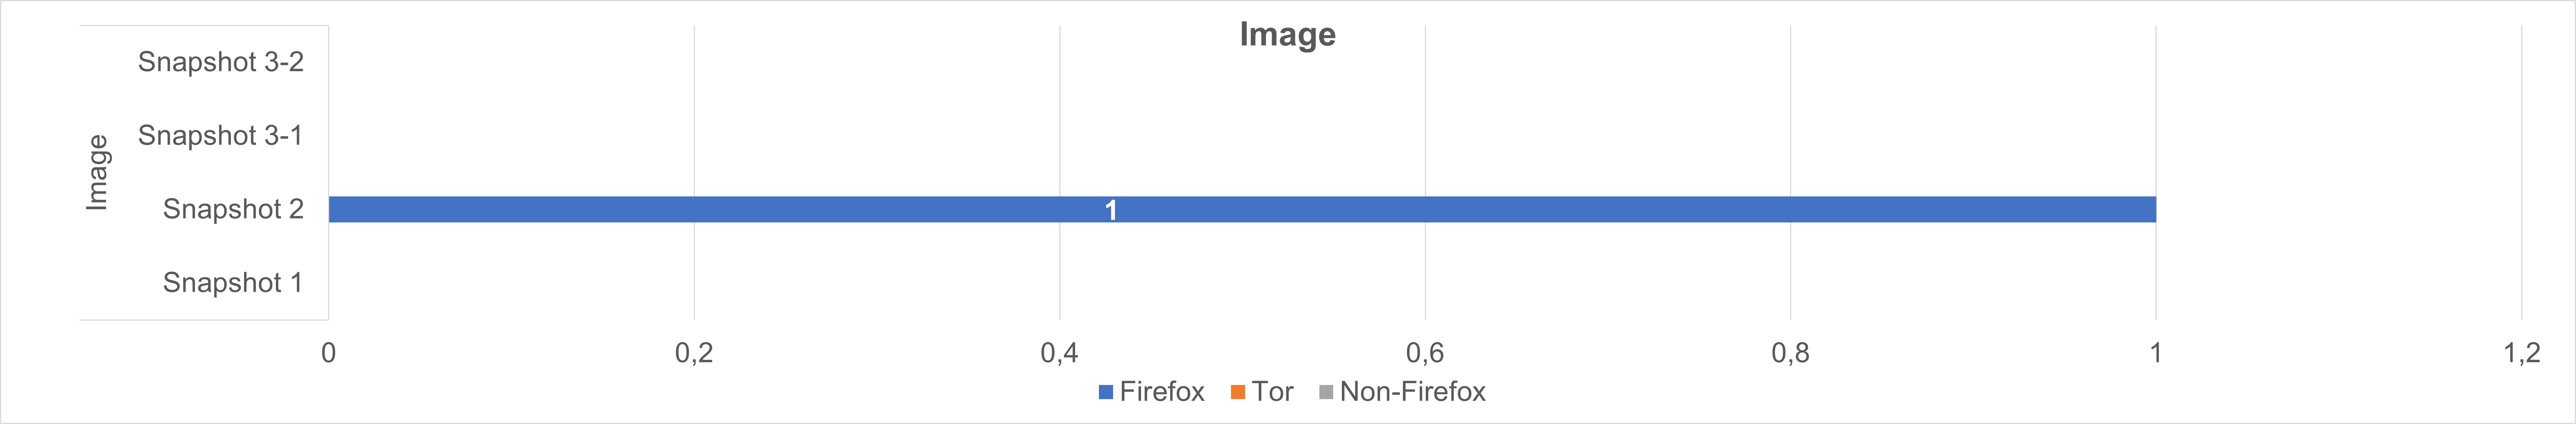
\includegraphics{bilder/volatility/tor/image.png}}}
		\label{chart:final-criteria}  
		\caption{Image}
	\end{figure}
	Analyse:
		> Hex-Wert von Donaukurier Bild wurde ein einzigees mal im 2. RAM Dump in einem Firefox Prozess gefunden
	

Zusammenfassung = Stacked Bar Chart:
\begin{figure}[h!]
	\centerline{\resizebox{\linewidth}{!}{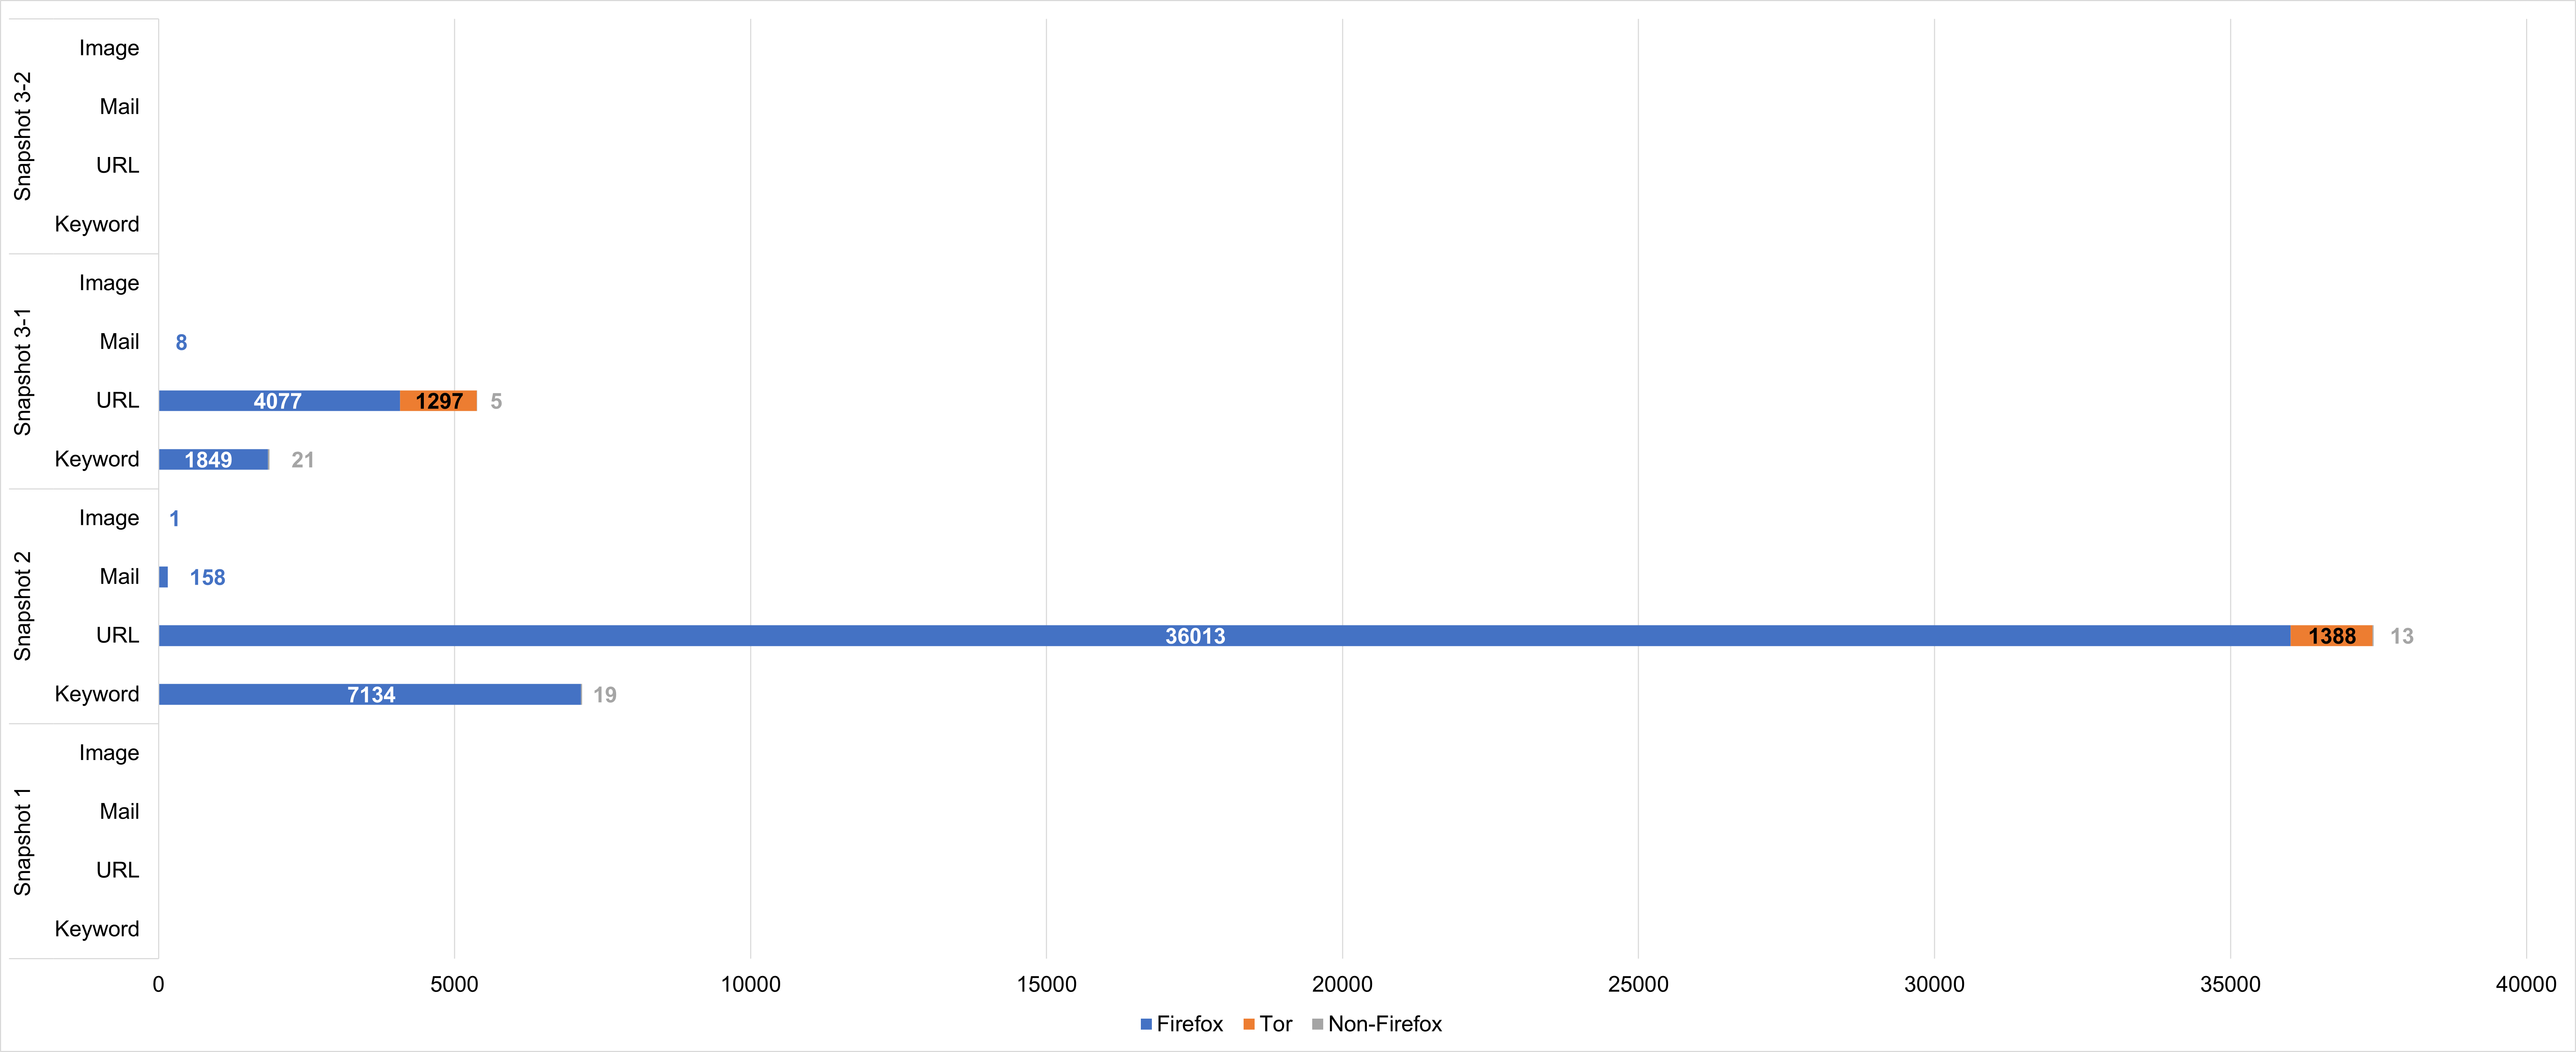
\includegraphics{bilder/volatility/tor/summary.png}}}
	\label{chart:final-criteria}  
	\caption{Summary}
\end{figure}
- PB Artefakte ausschließlich in RAM Dump 2 und 3-1 gefunden
- Nach Identitäts-Reset deutlich weniger Artefakte in vorhanden
- Am meisten URL-Artefakte gefunden, wobei mallofamerica.com dominant 
- HTML Artefakte wurden in keinem RAM Dump gefunden


TODO: Kreisdiagramme/Balkendiagramme mit Gesamtzahl an (Non-)Firefox Yarascan-Treffer erst im Vergleich mit Tor

\subsection*{Uncommon Locations}

Literatur:
%o Autopsy: \cite{Muir.2019}
%	•	Configuration files, downloaded files, and browserrelated data are recoverable from the file system.
%	•	Significant data-leakage from the browsing session occurred: HTTP header information, titles of web pages and an instance of a URL were found in registry files, system files, and unallocated space.
%o RAM-Analyse nach \cite{Muir.2019}:
%	•	Live-Analyse identifiziert auch nach dem Schließen und Deinstallieren des Browsers und Abmelden des Benutzers Spuren von Tor-Prozessen, einschließlich des absoluten Pfads zur Browser-Executable, des Benutzernamens und des Geräts, von dem es ausgeführt wurde.
%	•	The data-leakage contained the German word for ’search’ in reference to a Google search. This hints at the locale of the Tor server used to exit the network (exit relay).
%
%o RAM-Analyse nach \cite{Hariharan.2022}:
%	o	process was found to be firefox.exe
%	o	pslist and pstree: parent process was shown 
%	o	Belkasoft Ram Capturer: retrieve information about facebook
%	o	Cmdline: file path of the browser “E:/TorBrowser/Browser/firefox.exe” + name of process tor.exe and firefox.exe
%	o	Dlllist: DLL files of the executable files were not captured
%	o	Netscan: tor.exe + obfs4proxy.exe -> showed “LISTENING” connections to nonstandardized ports as output.
%	Yarascan: was able to retrieve all the browsing sessions
%o RAM-Analyse nach \cite{Sajan.2021} mit Volatility
%	•	process list extracted from the memory
%	•	registry hives been extracted from the memory dump
%	•	threads were extracted: “D:/VolatilityWorkbench/volatility.exe”–plugins=”D:/VolatilityWorkbench/profiles” pslistfilename =”C:/Users/username/Desktop/tor.raw” –profile=Win10x64 17763 –kdbg=0xf807606ac5e0
%	•	Handles: resources used by the process 5672
%	•	Dlls: These dlls can be found from prefetch file --> Can be found in “prefetch” file -> Analyzed with “winprefetchview”
%	•	Places.sqlite: SQLite viewer has been used to recover bookmarks and frequently visited sites even after uninstalling the application
%	•	Visited Websites: Using keyword search in Dump’s Hex
%
%o Registry:
%	> Shellactivites (siehe Firefox) \cite{Muir.2019}: instance of a URL were found in registry file
%	> \cite{Nelson.2020} The userassist key is located in the NTUSER.dat hive of the
%		 -> Registry and indicates the execution path of the program, as well as the number of times the program was executed 


%%%%%%%%%%%%%%%%%%%%%
% CHRISTOPH AB HIER %
%%%%%%%%%%%%%%%%%%%%%

\section{Chrome}\label{chap:ergebnisse-chrome}

Anschließend folgt die Analyse des Webbrowsers Chrome. Die Ergebnisse werden dabei wie in den beiden vorherigen Kapitel präsentiert.

\subsection*{Common Locations}\label{chap:ergebnisse-chrome-common-location}

Zuerst werden die Common Locations nach Artefakten des privaten Browsing-Szenarios untersucht. Dabei wird wieder zwischen Datei-Schreiboperationen aus den Process Monitor Logfiles und den SQLite-Datenbanken unterschieden, wie im [link kapitel] erläutert. Es konnten darin jedoch keine Artefakte gefunden werden.\\
Eine weitergehende Analyse aller Schreiboperationen sowie den Datenbänken ist im \autoref{chap:anhang-chrome-common-locations} detailliert aufgeführt.

\begin{comment} % Alles in Anhang nunter
o Autopsy Keyword-Suche: 
	> Chrome and Edge produced five artefacts as reported by both tools. (FTK, Autopsy) \cite{Gabet.2018}
		--> Artefakte werden nicht genannt!
	> only two temporary files (Figure 7) were recovered with Minitool Power Data Recovery but it was a dead end; Location: appdata/…/Chrome/…/ Preferences/RF1533fa.TMP \cite{Fayyad.2021}
	> pagefile.sys file showed no traces at all \cite{Said.2011}


Auch beim Chrome Browser werden zunächst die Ergebnisse der Schreiboperationen ausgewertet. Dargelegt sind diese in die folgenden zwei Unterkapiteln. 

\subsubsection*{Process Monitor Log 1}

Zunächst werden alle Schreiboperationen während des tatsächlichen Browsing-Szenarios analysiert. Dabei sind 148 Schreiboperationen aufgezeichnet worden. Nach Entfernen der Duplikate in den gleichen Dateipfaden waren es dann 42 verschiedene Dateien, welche beschrieben wurden. Einen Überblick über alle diese Dateien zeigt \autoref{tab:chrome-log-1-written-files}. Diese sind in verschiedene Kategorien aufgeteilt, was in der ersten Spalte zu sehen ist. Ob und welche Artefakte gefunden wurden zeugt die letzte Spalte. Nicht rekonstruierbar bedeutet, wie bereits erläutert, dass die Datei weder im Snapshot oder im RAM zu finden ist.

\begin{table}[ht]
	\centering
	\begin{adjustbox}{max width=\textwidth}
		\begin{tabular}{|l|l|l|l|l|}
			\hline
			Categories & Process Name & PID  & Path                                                                                                                                                                                                                                                                                                                               & Artefakte                  \\
			\hline\hline
			\multirow{6}{*}{Datenbanken und zugehörige journal-Dateien} & chrome.exe   & 764  & C:\textbackslash{}Users\textbackslash{}Forensik\textbackslash{}AppData\textbackslash{}Local\textbackslash{}Google\textbackslash{}Chrome\textbackslash{}User   Data\textbackslash{}Default\textbackslash{}History-journal                                                                                                           & Leere Datei (0 Bytes groß) \\
			& chrome.exe   & 764  & C:\textbackslash{}Users\textbackslash{}Forensik\textbackslash{}AppData\textbackslash{}Local\textbackslash{}Google\textbackslash{}Chrome\textbackslash{}User Data\textbackslash{}Default\textbackslash{}History                                                                                                                     & Keine Artefakte            \\
			\cline{2-5}
			& chrome.exe   & 764  & C:\textbackslash{}Users\textbackslash{}Forensik\textbackslash{}AppData\textbackslash{}Local\textbackslash{}Google\textbackslash{}Chrome\textbackslash{}User Data\textbackslash{}Default\textbackslash{}Web   Data-journal                                                                                                          & Leere Datei (0 Bytes groß) \\
			& chrome.exe   & 764  & C:\textbackslash{}Users\textbackslash{}Forensik\textbackslash{}AppData\textbackslash{}Local\textbackslash{}Google\textbackslash{}Chrome\textbackslash{}User Data\textbackslash{}Default\textbackslash{}Web Data                                                                                                                    & Keine Artefakte            \\
			\cline{2-5}
			& chrome.exe   & 396  & C:\textbackslash{}Users\textbackslash{}Forensik\textbackslash{}AppData\textbackslash{}Local\textbackslash{}Google\textbackslash{}Chrome\textbackslash{}User   Data\textbackslash{}Default\textbackslash{}Network\textbackslash{}Reporting and NEL-journal                                                                          & Leere Datei (0 Bytes groß) \\
			& chrome.exe   & 396  & C:\textbackslash{}Users\textbackslash{}Forensik\textbackslash{}AppData\textbackslash{}Local\textbackslash{}Google\textbackslash{}Chrome\textbackslash{}User   Data\textbackslash{}Default\textbackslash{}Network\textbackslash{}Reporting and NEL                                                                                  & Keine Artefakte            \\
			\hline
			\multirow{15}{*}{Temporäre Dateien (.tmp)} & chrome.exe   & 764  & C:\textbackslash{}Users\textbackslash{}Forensik\textbackslash{}AppData\textbackslash{}Local\textbackslash{}Google\textbackslash{}Chrome\textbackslash{}User   Data\textbackslash{}6f9e2d84-9a77-41e3-8955-b0c836f8fd0c.tmp                                                                                                         & Nicht rekonstruierbar      \\
			& chrome.exe   & 764  & C:\textbackslash{}Users\textbackslash{}Forensik\textbackslash{}AppData\textbackslash{}Local\textbackslash{}Google\textbackslash{}Chrome\textbackslash{}User   Data\textbackslash{}a0ea17f1-38e8-48e0-a2f4-98e9be6a6dd3.tmp                                                                                                         & Nicht rekonstruierbar      \\
			& chrome.exe   & 396  & C:\textbackslash{}Users\textbackslash{}Forensik\textbackslash{}AppData\textbackslash{}Local\textbackslash{}Google\textbackslash{}Chrome\textbackslash{}User   Data\textbackslash{}Default\textbackslash{}Network\textbackslash{}a3ab3887-9ed6-45e7-a1bc-e0a34974b332.tmp                                                           & Nicht rekonstruierbar      \\
			& chrome.exe   & 764  & C:\textbackslash{}Users\textbackslash{}Forensik\textbackslash{}AppData\textbackslash{}Local\textbackslash{}Google\textbackslash{}Chrome\textbackslash{}User   Data\textbackslash{}b23e8f25-4bfb-4625-a9d5-836ff096b671.tmp                                                                                                         & Nicht rekonstruierbar      \\
			& chrome.exe   & 764  & C:\textbackslash{}Users\textbackslash{}Forensik\textbackslash{}AppData\textbackslash{}Local\textbackslash{}Google\textbackslash{}Chrome\textbackslash{}User   Data\textbackslash{}2da074d0-9208-4026-b970-d7261bd389c3.tmp                                                                                                         & Nicht rekonstruierbar      \\
			& chrome.exe   & 764  & C:\textbackslash{}Users\textbackslash{}Forensik\textbackslash{}AppData\textbackslash{}Local\textbackslash{}Google\textbackslash{}Chrome\textbackslash{}User   Data\textbackslash{}44a1b7b5-40eb-4265-8d3e-b55d21084e65.tmp                                                                                                         & Nicht rekonstruierbar      \\
			& chrome.exe   & 764  & C:\textbackslash{}Users\textbackslash{}Forensik\textbackslash{}AppData\textbackslash{}Local\textbackslash{}Google\textbackslash{}Chrome\textbackslash{}User   Data\textbackslash{}1f7ba833-406a-40cf-b107-6e391f4bd1d3.tmp                                                                                                         & Nicht rekonstruierbar      \\
			& chrome.exe   & 764  & C:\textbackslash{}Users\textbackslash{}Forensik\textbackslash{}AppData\textbackslash{}Local\textbackslash{}Google\textbackslash{}Chrome\textbackslash{}User   Data\textbackslash{}97615fa9-9081-43b0-af51-534da2fd8cb4.tmp                                                                                                         & Nicht rekonstruierbar      \\
			& chrome.exe   & 764  & C:\textbackslash{}Users\textbackslash{}Forensik\textbackslash{}AppData\textbackslash{}Local\textbackslash{}Google\textbackslash{}Chrome\textbackslash{}User   Data\textbackslash{}fbd23442-8e9b-47cb-95e6-9da65df2c42e.tmp                                                                                                         & Nicht rekonstruierbar      \\
			& chrome.exe   & 764  & C:\textbackslash{}Users\textbackslash{}Forensik\textbackslash{}AppData\textbackslash{}Local\textbackslash{}Google\textbackslash{}Chrome\textbackslash{}User   Data\textbackslash{}fecad46f-9d32-40a2-aa3c-7b1cc275a5e2.tmp                                                                                                         & Nicht rekonstruierbar      \\
			& chrome.exe   & 764  & C:\textbackslash{}Users\textbackslash{}Forensik\textbackslash{}AppData\textbackslash{}Local\textbackslash{}Google\textbackslash{}Chrome\textbackslash{}User   Data\textbackslash{}e5e0606b-51a1-44ba-a8f9-80f1cf5c48a3.tmp                                                                                                         & Nicht rekonstruierbar      \\
			& chrome.exe   & 764  & C:\textbackslash{}Users\textbackslash{}Forensik\textbackslash{}AppData\textbackslash{}Local\textbackslash{}Google\textbackslash{}Chrome\textbackslash{}User   Data\textbackslash{}c029e5f2-88df-4271-bc24-2c50db41cc89.tmp                                                                                                         & Nicht rekonstruierbar      \\
			& chrome.exe   & 396  & C:\textbackslash{}Users\textbackslash{}Forensik\textbackslash{}AppData\textbackslash{}Local\textbackslash{}Google\textbackslash{}Chrome\textbackslash{}User   Data\textbackslash{}Default\textbackslash{}Network\textbackslash{}184cc287-bc19-4faf-bd09-fdfc1ff1c6b8.tmp                                                           & Nicht rekonstruierbar      \\
			& chrome.exe   & 764  & C:\textbackslash{}Users\textbackslash{}Forensik\textbackslash{}AppData\textbackslash{}Local\textbackslash{}Google\textbackslash{}Chrome\textbackslash{}User   Data\textbackslash{}Default\textbackslash{}9a105eba-925a-4d38-994f-c59962a8a60c.tmp                                                                                  & Nicht rekonstruierbar      \\
			& chrome.exe   & 764  & C:\textbackslash{}Users\textbackslash{}Forensik\textbackslash{}AppData\textbackslash{}Local\textbackslash{}Google\textbackslash{}Chrome\textbackslash{}User   Data\textbackslash{}8b2096fb-9e68-4a4c-9df5-3dd0949aa210.tmp                                                                                                         & Nicht rekonstruierbar      \\
			\hline
			\multirow{8}{*}{Temporäre Bilddateien (.png)} & chrome.exe   & 764  & C:\textbackslash{}Users\textbackslash{}Forensik\textbackslash{}AppData\textbackslash{}Local\textbackslash{}Google\textbackslash{}Chrome\textbackslash{}User Data\textbackslash{}Default\textbackslash{}Web   Applications\textbackslash{}Temp\textbackslash{}scoped\_dir764\_530297989\textbackslash{}Icons\textbackslash{}32.png  & Nicht rekonstruierbar      \\
			& chrome.exe   & 764  & C:\textbackslash{}Users\textbackslash{}Forensik\textbackslash{}AppData\textbackslash{}Local\textbackslash{}Google\textbackslash{}Chrome\textbackslash{}User Data\textbackslash{}Default\textbackslash{}Web   Applications\textbackslash{}Temp\textbackslash{}scoped\_dir764\_530297989\textbackslash{}Icons\textbackslash{}48.png  & Nicht rekonstruierbar      \\
			& chrome.exe   & 764  & C:\textbackslash{}Users\textbackslash{}Forensik\textbackslash{}AppData\textbackslash{}Local\textbackslash{}Google\textbackslash{}Chrome\textbackslash{}User Data\textbackslash{}Default\textbackslash{}Web   Applications\textbackslash{}Temp\textbackslash{}scoped\_dir764\_530297989\textbackslash{}Icons\textbackslash{}64.png  & Nicht rekonstruierbar      \\
			& chrome.exe   & 764  & C:\textbackslash{}Users\textbackslash{}Forensik\textbackslash{}AppData\textbackslash{}Local\textbackslash{}Google\textbackslash{}Chrome\textbackslash{}User Data\textbackslash{}Default\textbackslash{}Web   Applications\textbackslash{}Temp\textbackslash{}scoped\_dir764\_530297989\textbackslash{}Icons\textbackslash{}96.png  & Nicht rekonstruierbar      \\
			& chrome.exe   & 764  & C:\textbackslash{}Users\textbackslash{}Forensik\textbackslash{}AppData\textbackslash{}Local\textbackslash{}Google\textbackslash{}Chrome\textbackslash{}User Data\textbackslash{}Default\textbackslash{}Web   Applications\textbackslash{}Temp\textbackslash{}scoped\_dir764\_530297989\textbackslash{}Icons\textbackslash{}128.png & Nicht rekonstruierbar      \\
			& chrome.exe   & 764  & C:\textbackslash{}Users\textbackslash{}Forensik\textbackslash{}AppData\textbackslash{}Local\textbackslash{}Google\textbackslash{}Chrome\textbackslash{}User Data\textbackslash{}Default\textbackslash{}Web   Applications\textbackslash{}Temp\textbackslash{}scoped\_dir764\_530297989\textbackslash{}Icons\textbackslash{}192.png & Nicht rekonstruierbar      \\
			& chrome.exe   & 764  & C:\textbackslash{}Users\textbackslash{}Forensik\textbackslash{}AppData\textbackslash{}Local\textbackslash{}Google\textbackslash{}Chrome\textbackslash{}User Data\textbackslash{}Default\textbackslash{}Web   Applications\textbackslash{}Temp\textbackslash{}scoped\_dir764\_530297989\textbackslash{}Icons\textbackslash{}256.png & Nicht rekonstruierbar      \\
			& chrome.exe   & 764  & C:\textbackslash{}Users\textbackslash{}Forensik\textbackslash{}AppData\textbackslash{}Local\textbackslash{}Google\textbackslash{}Chrome\textbackslash{}User Data\textbackslash{}Default\textbackslash{}Web   Applications\textbackslash{}Temp\textbackslash{}scoped\_dir764\_530297989\textbackslash{}Icons\textbackslash{}512.png & Nicht rekonstruierbar      \\
			\hline
			\multirow{5}{*}{data\_1 Dateien} & chrome.exe   & 764  & C:\textbackslash{}Users\textbackslash{}Forensik\textbackslash{}AppData\textbackslash{}Local\textbackslash{}Google\textbackslash{}Chrome\textbackslash{}User   Data\textbackslash{}Default\textbackslash{}GPUCache\textbackslash{}data\_1                                                                                           & Keine Artefakte            \\
			& chrome.exe   & 764  & C:\textbackslash{}Users\textbackslash{}Forensik\textbackslash{}AppData\textbackslash{}Local\textbackslash{}Google\textbackslash{}Chrome\textbackslash{}User   Data\textbackslash{}Default\textbackslash{}DawnCache\textbackslash{}data\_1                                                                                          & Keine Artefakte            \\
			& chrome.exe   & 764  & C:\textbackslash{}Users\textbackslash{}Forensik\textbackslash{}AppData\textbackslash{}Local\textbackslash{}Google\textbackslash{}Chrome\textbackslash{}User   Data\textbackslash{}ShaderCache\textbackslash{}data\_1                                                                                                               & Keine Artefakte            \\
			& chrome.exe   & 764  & C:\textbackslash{}Users\textbackslash{}Forensik\textbackslash{}AppData\textbackslash{}Local\textbackslash{}Google\textbackslash{}Chrome\textbackslash{}User   Data\textbackslash{}GrShaderCache\textbackslash{}data\_1                                                                                                             & Keine Artefakte            \\
			& chrome.exe   & 396  & C:\textbackslash{}Users\textbackslash{}Forensik\textbackslash{}AppData\textbackslash{}Local\textbackslash{}Google\textbackslash{}Chrome\textbackslash{}User   Data\textbackslash{}Default\textbackslash{}Cache\textbackslash{}Cache\_Data\textbackslash{}data\_1                                                                   & Keine Artefakte            \\
			\hline
			\multirow{2}{*}{LevelDB 000003.log Dateien} & chrome.exe   & 764  & C:\textbackslash{}Users\textbackslash{}Forensik\textbackslash{}AppData\textbackslash{}Local\textbackslash{}Google\textbackslash{}Chrome\textbackslash{}User   Data\textbackslash{}Default\textbackslash{}shared\_proto\_db\textbackslash{}000003.log                                                                               & Keine Artefakte            \\
			& chrome.exe   & 764  & C:\textbackslash{}Users\textbackslash{}Forensik\textbackslash{}AppData\textbackslash{}Local\textbackslash{}Google\textbackslash{}Chrome\textbackslash{}User Data\textbackslash{}Default\textbackslash{}Sync   Data\textbackslash{}LevelDB\textbackslash{}000003.log                                                                & Keine Artefakte            \\
			\hline\hline
			\multirow{3}{*}{Shader Cache Dateien} & chrome.exe   & 8904 & C:\textbackslash{}Users\textbackslash{}Forensik\textbackslash{}AppData\textbackslash{}Local\textbackslash{}D3DSCache\textbackslash{}cb00da9ba77862e\textbackslash{}F4EB2D6C-ED2B-4BDD-AD9D-F913287E6768.idx                                                                                                                        & Keine Artefakte            \\
			& chrome.exe   & 8904 & C:\textbackslash{}Users\textbackslash{}Forensik\textbackslash{}AppData\textbackslash{}Local\textbackslash{}D3DSCache\textbackslash{}cb00da9ba77862e\textbackslash{}F4EB2D6C-ED2B-4BDD-AD9D-F913287E6768.lock                                                                                                                       & Keine Artefakte            \\
			& chrome.exe   & 8904 & C:\textbackslash{}Users\textbackslash{}Forensik\textbackslash{}AppData\textbackslash{}Local\textbackslash{}D3DSCache\textbackslash{}cb00da9ba77862e\textbackslash{}F4EB2D6C-ED2B-4BDD-AD9D-F913287E6768.val                                                                                                                      & Keine Artefakte            \\
			\hline
			\multirow{3}{*}{Windows dictionary files} & chrome.exe   & 764  & C:\textbackslash{}Users\textbackslash{}Forensik\textbackslash{}AppData\textbackslash{}Roaming\textbackslash{}Microsoft\textbackslash{}Spelling\textbackslash{}de-DE\textbackslash{}default.dic                                                                                                                                     & Keine Artefakte            \\
			& chrome.exe   & 764  & C:\textbackslash{}Users\textbackslash{}Forensik\textbackslash{}AppData\textbackslash{}Roaming\textbackslash{}Microsoft\textbackslash{}Spelling\textbackslash{}de-DE\textbackslash{}default.exc                                                                                                                                     & Keine Artefakte            \\
			& chrome.exe   & 764  & C:\textbackslash{}Users\textbackslash{}Forensik\textbackslash{}AppData\textbackslash{}Roaming\textbackslash{}Microsoft\textbackslash{}Spelling\textbackslash{}de-DE\textbackslash{}default.acl                                                                                                                                     & Keine Artefakte \\
			\hline           
		\end{tabular}
	\end{adjustbox}
	\caption{Tabelle mit allen Schreiboperationen des ersten ProcessMonitor-Logs}
	\label{tab:chrome-log-1-written-files}
\end{table}

Die verschiedenen Kategorien aus der ersten Spalte werden unterschiedlich analysiert. Im Folgenden wird zu jeder Kategorie das Vorgehen erklärt und der Inhalt der Daten, bzw. wofür diese von Chrome verwendet werden, erläutert.

\begin{sloppypar}
Zunächst geht es um die Datenbanken und die dazugehörigen journal-Dateien. Chrome speichert Informationen bzgl. des Browsings wie den Verlauf oder Cookies nicht wie Firefox in direkt als solche erkennbare .sqlte Dateien, sondern als Dateien ohne spezielle Endungen. Diese enthalten am Anfang der Datei den header string \glqq{}SQLite format 3\grqq{}, was auf eine SQLite-Datenbank hinweist \cite{SQLiteFileFormat}, was in [link pic] zu sehen ist. Autopsy erkennt dies auch und es ist mittels des \textit{Application} Tabs möglich, diese direkt in Autopsy zu analysieren. [link pic] zeigt dies. Außerdem befinden sich neben den eigentlichen Datenbanken noch gleichnamige Dateien mit dem Zusatz \textit{-journal} am Ende. Diese sind sogenannte \glqq{}Rollback Journals\grqq{} und sind relevant für atomare Commit- und Rollback-Funktionen \cite{SQLiteTempfiles}. Da diese -journal Dateien jedoch alle 0 Bytes groß waren, konnte hier kein Artefakt gefunden werden. Auch die Analyse der eigentlichen Datenbanken direkt in Autopsy und zusätzlich mittels des DB-Browsers lieferte hier keine Ergebnisse. Die relevanten Datenbanken werden später [link nach unten] nochmals genauer untersucht.\\
Anschließend wurde Temporäre Dateien, einmal mit der Endung \textit{.tmp}, und weitere temporäre Bilddateien mit der Endung \textit{.png}, geschrieben. Davon kann jedoch keine Datei rekonstruiert werden, wodurch hier kein Artefakt gefunden werden kann.\\
Als nächstes werden Dateien mit dem Namen \textit{data\_1} analysiert. Diese sind alle 270.336 Bytes groß und enthalten, bis auf die Datei, welche im Cache\textbackslash{}Cache\_Data Ordner geschrieben wird, keine erkennbaren Zeichenketten und sind großteils leer (0-Bytes). Auch die Datei im Cache-Ordner weißt nur standard Google HTTPS Adressen. Hierin konnte auch kein Artefakt gefunden werden.\\
Auch wurden noch \textit{000003.log}-Dateien geschrieben. Diese sind Teil eines LevelDB-Schlüsselwertespeichers \cite{LevelDBGithub,LevelDBCCL} . Mithife von HxD und einer Analyse mittels eines selbst erstellen Python-Scripts zur Ausgabe der Schlüssel-Werte-Paare der Ordner, welche die .log und weitere LevelDB spezifische Dateien enthält, kann auch in diesen Ordner bzw. Dateien auch keine Artefakte gefunden werden.

Alle zuvor aufgeführten Dateien sind im Browser-Verzeichnis AppData\textbackslash{}Local\textbackslash{}Google\textbackslash{}Chrome\textbackslash{}User Data\textbackslash{} zu finden. Dies wird auch als Browser-spezifischer Pfad oder Common location bezeichnet. Alle folgenden Schreiboperationen wurden außerhalb dieses Ordners durchgeführt. Dies ist in \autoref{tab:chrome-log-1-written-files} auch graphisch nochmals durch eine zusätzliche Linie abgetrennt.\end{sloppypar}

In den browser-unspezifischen Pfaden wurden einmal Shader-Cache Dateien geschrieben. Diese enthalten jedoch keine Artefakte. Außerdem wurden noch Dateien beschrieben, welche auf das Windows 10 Wörterbuch zurückzuführen sind \cite{DictionaryWin10Files}. All diese Dateien enthalten jedoch auch keine Browsing-Artefakte.

Zusammenfassend können also im ersten Prozessor-Log keine auf das Browsingszenario zurückzuführenden Artefakte gefunden werden.

\subsubsection*{Process Monitor Log 2}

Während des Schließens des Prozessors fanden insgesamt 30 Schreiboperationen durch Chrome statt. Das Entfernen von Duplikaten zeigt, dass 14 Dateien beschrieben wurden. Diese befinden sich bei dem zweiten Log alle im browserspezifischen Ordner AppData\textbackslash{}Local\textbackslash{}Google\textbackslash{}Chrome\textbackslash{}User Data\textbackslash{}. \autoref{tab:chrome-log-2-written-files} zeigt eine Überblick über diese wieder mit Angabe, ob Artefakte gefunden werden können.

\begin{table}[ht]
	\centering
	\begin{adjustbox}{max width=\textwidth}
		\begin{tabular}{|l|l|l|l|l|}
			\hline
			Categories & Process Name & PID  & Path                                                                                                                                                                                                                                                                                                                               & Artefakte                  \\
			\hline\hline
			Crashpad settings-Datei & chrome.exe   & 6152 & C:\textbackslash{}Users\textbackslash{}Forensik\textbackslash{}AppData\textbackslash{}Local\textbackslash{}Google\textbackslash{}Chrome\textbackslash{}User   Data\textbackslash{}Crashpad\textbackslash{}settings.dat                                                                                                                                                                & Keine Artefakte            \\
			\hline
			\multirow{5}{*}{Temporäre Dateien (.tmp)} & chrome.exe   & 6152 & C:\textbackslash{}Users\textbackslash{}Forensik\textbackslash{}AppData\textbackslash{}Local\textbackslash{}Google\textbackslash{}Chrome\textbackslash{}User   Data\textbackslash{}35debf2e-9a97-4829-b0d1-2c6efb7246bc.tmp                                                                                                                                                            & Nicht rekonstruierbar      \\
			& chrome.exe   & 6152 & C:\textbackslash{}Users\textbackslash{}Forensik\textbackslash{}AppData\textbackslash{}Local\textbackslash{}Google\textbackslash{}Chrome\textbackslash{}User   Data\textbackslash{}4dce7d9d-2753-424d-ad13-eb84e1ea9326.tmp                                                                                                                                                            & Nicht rekonstruierbar      \\
			& chrome.exe   & 6152 & C:\textbackslash{}Users\textbackslash{}Forensik\textbackslash{}AppData\textbackslash{}Local\textbackslash{}Google\textbackslash{}Chrome\textbackslash{}User   Data\textbackslash{}Default\textbackslash{}51ff0ac1-e188-4c8a-8b3d-891f326bb890.tmp                                                                                                                                     & Nicht rekonstruierbar      \\
			& chrome.exe   & 6152 & C:\textbackslash{}Users\textbackslash{}Forensik\textbackslash{}AppData\textbackslash{}Local\textbackslash{}Google\textbackslash{}Chrome\textbackslash{}User   Data\textbackslash{}52837c44-01bc-43d1-b859-0fe50c823372.tmp                                                                                                                                                            & Nicht rekonstruierbar      \\
			& chrome.exe   & 7012 & C:\textbackslash{}Users\textbackslash{}Forensik\textbackslash{}AppData\textbackslash{}Local\textbackslash{}Google\textbackslash{}Chrome\textbackslash{}User   Data\textbackslash{}Default\textbackslash{}Storage\textbackslash{}ext\textbackslash{}nmmhkkegccagdldgiimedpiccmgmieda\textbackslash{}def\textbackslash{}Network\textbackslash{}c280cbe5-825f-482f-8c5f-e4b0f0e8d560.tmp & Keine Artefakte            \\
			\hline
			\multirow{2}{*}{Datenbank und zugehörige journal-Datei} & chrome.exe   & 6152 & C:\textbackslash{}Users\textbackslash{}Forensik\textbackslash{}AppData\textbackslash{}Local\textbackslash{}Google\textbackslash{}Chrome\textbackslash{}User   Data\textbackslash{}Default\textbackslash{}History-journal                                                                                                                                                              & Leere Datei (0 Bytes groß) \\
			& chrome.exe   & 6152 & C:\textbackslash{}Users\textbackslash{}Forensik\textbackslash{}AppData\textbackslash{}Local\textbackslash{}Google\textbackslash{}Chrome\textbackslash{}User   Data\textbackslash{}Default\textbackslash{}History                                                                                                                                                                      & Keine Artefakte            \\
			\hline
			JSON-Datei & chrome.exe   & 6152 & C:\textbackslash{}Users\textbackslash{}Forensik\textbackslash{}AppData\textbackslash{}Local\textbackslash{}Google\textbackslash{}Chrome\textbackslash{}User Data\textbackslash{}Variations                                                                                                                                                                                            & Keine Artefakte            \\
			\hline
			LevelDB 000003.log Datei & chrome.exe   & 5484 & C:\textbackslash{}Users\textbackslash{}Forensik\textbackslash{}AppData\textbackslash{}Local\textbackslash{}Google\textbackslash{}Chrome\textbackslash{}User   Data\textbackslash{}Default\textbackslash{}Session Storage\textbackslash{}000003.log                                                                                                                                    & Keine Artefakte            \\
			\hline
			\multirow{3}{*}{data\_1 Dateien} & chrome.exe   & 7012 & C:\textbackslash{}Users\textbackslash{}Forensik\textbackslash{}AppData\textbackslash{}Local\textbackslash{}Google\textbackslash{}Chrome\textbackslash{}User   Data\textbackslash{}Default\textbackslash{}Cache\textbackslash{}Cache\_Data\textbackslash{}data\_1                                                                                                                      & Keine Artefakte            \\
			& chrome.exe   & 6152 & C:\textbackslash{}Users\textbackslash{}Forensik\textbackslash{}AppData\textbackslash{}Local\textbackslash{}Google\textbackslash{}Chrome\textbackslash{}User   Data\textbackslash{}GrShaderCache\textbackslash{}data\_1                                                                                                                                                                & Keine Artefakte            \\
			& chrome.exe   & 6152 & C:\textbackslash{}Users\textbackslash{}Forensik\textbackslash{}AppData\textbackslash{}Local\textbackslash{}Google\textbackslash{}Chrome\textbackslash{}User   Data\textbackslash{}ShaderCache\textbackslash{}data\_1                                                                                                                                                                  & Keine Artefakte            \\
			\hline
			Millisekunden Chrome shutdown Zeit & chrome.exe   & 6152 & C:\textbackslash{}Users\textbackslash{}Forensik\textbackslash{}AppData\textbackslash{}Local\textbackslash{}Google\textbackslash{}Chrome\textbackslash{}User   Data\textbackslash{}chrome\_shutdown\_ms.txt                                                                                                                                                                            & Keine Artefakte\\           
			
			\hline           
			\end{tabular}
		\end{adjustbox}
	\caption{Tabelle mit allen Schreiboperationen des zweiten ProcessMonitor-Logs}
\label{tab:chrome-log-2-written-files}
\end{table}

Die Datei \textit{settings.dat} im Crashpad Ordner ist Teil der Crashpad library, welche den Maschinen- und Programmzustand im Falle eines Prozessabsturzes erfasst und einen Absturzbericht an einen Backend-Server übermittelt \cite{CrashpadOverviewDesign}. Die (binäre) Datei an sich beinhaltet dabei die Einstellungen für die Bibliothek \cite{CrashpadOverviewDesign}. Diese Datei beinhaltet jedoch keine Browsing-Artefakte. \\
Weiterhin wurden wieder temporäre Dateien geschrieben, welche bis auf eine Datei nicht rekonstruierbar sind. Diese Eine enthält jedoch keine Artefakte. \\
Die Datenbank \textit{History} sowie die dazugehörige \textit{-journal}-Datei zeigten auch wieder keine Artefakte.
Die Datei \textit{Variations} direkt im Google\textbackslash{}Chrome\textbackslash{}User Data\textbackslash{}-Ordner ist der Dateistruktur nach eine JSON-Datei. Diese enthält aber auch keinerlei Informationen über das durchgeführte Browsing-Szenario.\\
Auch wird wieder eine \textit{000003.log}-Datei geschrieben, welche aber wieder keine Artefakte enthält.\\
Gleiches gilt für die geschriebenen \textit{data\_1}-Dateien.\\
Zuletzt wurde noch eine Textdatei namens \textit{chrome\_shotdown\_ms.txt} geschrieben. Diese enthält die Zeit in Millisekunden, welche Chrome für das Schießen benötigt \cite{ChromiumShutdownMSTxtWebpageDoku}. Dort fanden sich neben der Zeit in Millisekunden keine weiteren Artefakte.

Auch im zweiten Prozessor-Log können schließlich keine Artefakte gefunden werden. Somit werden weder während des Browsings noch beim Schließen des Chrome Browsers Informationen des definierten Browsing-Szenarios in keine Dateien auf die Festplatte geschrieben. 

\subsubsection*{Databases}

Welche Datenbanken sind wann vorhanden? Was verändert sich über die Zeit? Textuell + Tabellarisch zeigen!

\subsection*{Registry}

\subsubsection*{Process Monitor}

Zuerst die im Process Monitor aufgeze

\subsubsection*{Hives-Extraction inklusive Analyse}

Dann Auslesen der bereits in [link] dargestellten Hives + Einlesen in Registry Explorer. Liefert bei allen 3 betrachteten Snapshots keine Ergebnisse

\subsection*{Black-Box Analyse/Uncommon Locations}

\subsubsection*{Analyse mit Autopsy}

\subsubsection*{Analyse mit Volatility}

Jeweils schöne Tabellen hierzu:

Keywords\\
URL\\
Mail \\
HTTP + Vorgehen der Abstraktion inkl. Screenshots hier

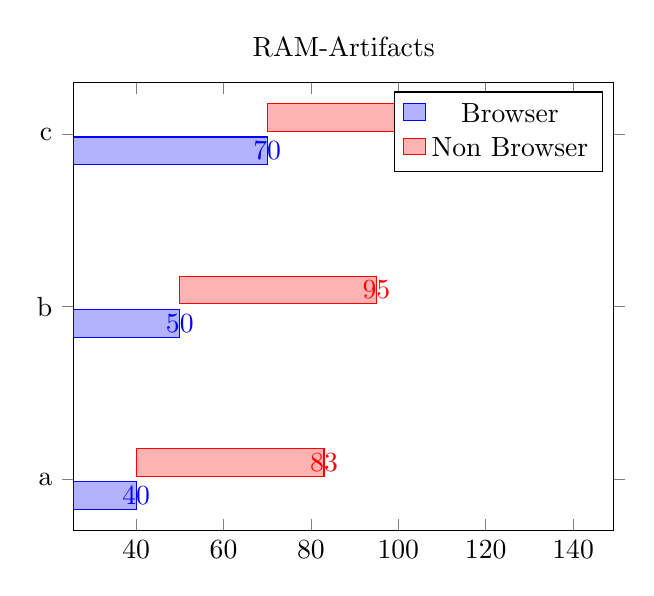
\begin{tikzpicture}
	\begin{axis}[title=RAM-Artifacts,
		xbar,enlargelimits=0.15,nodes near coords,
		symbolic y coords={a,b,c},ytick=data,
		xbar stacked,
		]
		\addplot coordinates
		{(40,a) (50,b) (70,c)};
		\addplot coordinates
		{(43,a) (45,b) (65,c)};
	\legend{Browser, Non Browser}
	\end{axis}
\end{tikzpicture}


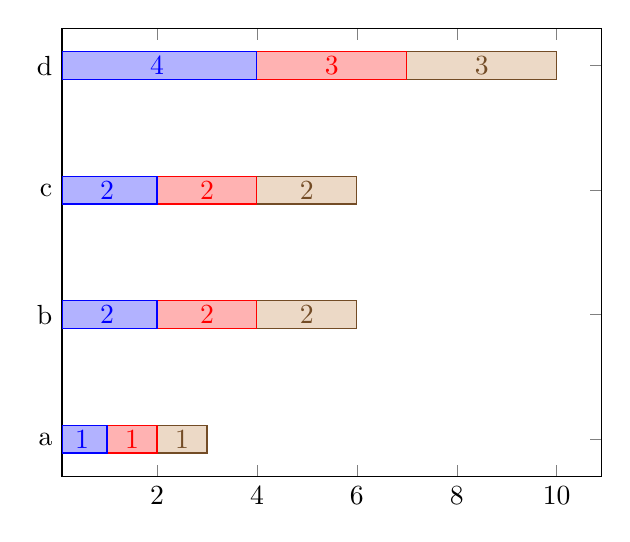
\begin{tikzpicture}
	\begin{axis}[xbar stacked,
		nodes near coords,
		symbolic y coords={a,b,c,d},
		]
		\addplot coordinates
		{(1,a) (2,b) (2,c) (4,d)};
		\addplot coordinates
		{(1,a) (2,b) (2,c) (3,d)};
		\addplot coordinates
		{(1,a) (2,b) (2,c) (3,d)};
	\end{axis}
\end{tikzpicture}

\begin{bchart}[max=8]
	\bcbar[text=A,label=1st label,color=yellow]{6}
	\bcbar[text=B,color=red!50]{3}
	\bcbar[text=C,color=green!60!blue]{4}
	\bcskip{15mm}
	\bcbar[text=D,color=blue]{6}
\end{bchart}

Image + Summary Tabellen hier am Ende no!

\end{comment}

\subsection*{Uncommon Locations}\label{chap:ergebnisse-chrome-uncommon-locations}

Nachfolgend werden die Ergebnisse der Uncommon Location Analyse des Chrome Browsers dargelegt. Dafür werden die beiden Forensik-Programme Autopsy und Volatility verwendet.

\subsubsection*{Analyse mit Autopsy}\label{chap:ergebnisse-chrome-uncommon-autopsy}

Auch in Autopsy konnten keine Artefakte der durchgeführten Browsing-Session gefunden werden, weder durch die Substringsuche, noch durch die Analyse der von Autopsy kategorisierten Dateien. Eine weitergehende Analyse einiger kategorisierter Dateien ist im \autoref{chap:anhang-chrome-uncommon-autopsy} zu finden.

\subsubsection*{Analyse mit Volatility}\label{chap:ergebnisse-chrome-uncommon-volatility}

Nachdem bis jetzt noch keine Artefakte gefunden werden konnten, folgen nun die Analyseergebnisse des Hauptspeichers (RAM) mittels des Forensik-Tools Volatility. Im RAM konnten schließlich Artefakte gefunden werden. Diese wurden mittels des Volatility Plugins Yarascan identifiziert, wobei die Yara-Regeln aus [link Kapitel] verwendet wurden. Zusätzlich zu den erkannten Strings spielt auch noch die PID eine entscheidende Rolle, da damit der Treffer entweder dem Browser oder einem anderen Prozess eindeutig zuordnet werden kann. Die Ergebnisse dieser String-Suche werden nachfolgend dargelegt.

\paragraph*{Yara-Regel \glqq{}HTML\grqq{}}\label{chap:ergebnisse-chrome-uncommon-volatility-html}

Im Gegensatz zu den Ergebnissen der Analyse der beiden vorherigen Browser, konnte ein HTML-Fragment bei Chrome im Arbeitsspeicher gefunden werden. Wie in \autoref{chart:chrome-volatility-htmls} dargestellt, wird der String \glqq{}>Themen:\grqq{} im zweiten RAM-Dump in einem Chrome-Prozess gefunden.

\begin{table}[h!]
	\resizebox{\linewidth}{!}{
		\begin{tabular}{l}	
			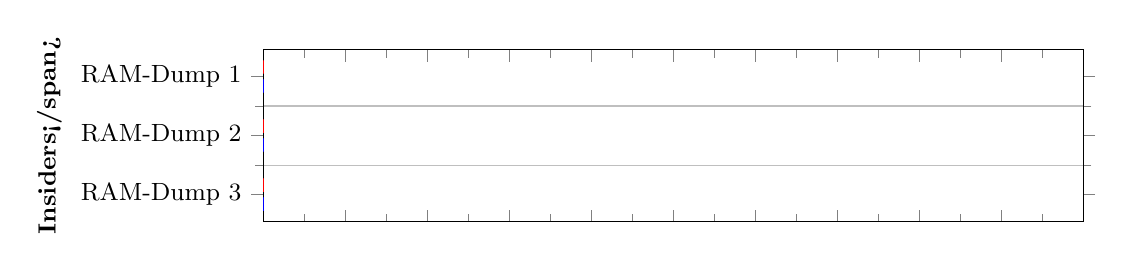
\begin{tikzpicture}
				\begin{axis}[
					xbar,
					width=12cm, 
					height=3cm, 
					ylabel style={align=center}, ylabel=\textbf{Insiders</span>},
					y=0.75cm,
					symbolic y coords={RAM-Dump 3, RAM-Dump 2, RAM-Dump 1},
					label style={font=\small},
					tick label style={font=\small},
					ytick=data,
					xticklabels={,,},
					xmin = 0,
					xmax = 5,
					nodes near coords, 
					nodes near coords align={horizontal},
					nodes near coords style={font=\tiny},
					nodes near coords={\pgfmathfloatifflags{\pgfplotspointmeta}{0}{}{\pgfmathprintnumber{\pgfplotspointmeta}}},
					bar width=.17cm,
					enlarge y limits={abs=2*\pgfplotbarwidth},
					scaled x ticks=false,
					legend style={
						at={(0.5,-0.1)},
						anchor=north
					},
					legend columns=3,
					yminorgrids = true,minor tick num=1
					]
					\addplot coordinates {
						(0,RAM-Dump 3) (0,RAM-Dump 2) (0,RAM-Dump 1)
					};
					\addplot coordinates {
						(0,RAM-Dump 3) (0,RAM-Dump 2) (0,RAM-Dump 1)
					};
				\end{axis}
			\end{tikzpicture}
			\\[-7pt]
			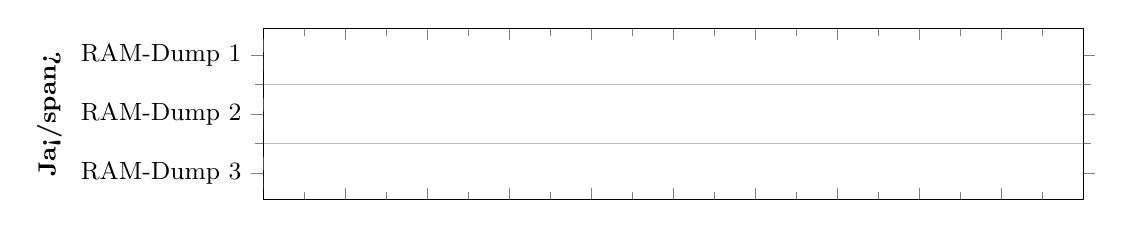
\begin{tikzpicture}
				\begin{axis}[
					xbar,
					width=12cm, 
					height=3cm, 
					ylabel style={align=center}, ylabel=\textbf{Ja</span>},
					y=0.75cm,
					symbolic y coords={RAM-Dump 3, RAM-Dump 2, RAM-Dump 1},
					label style={font=\small},
					tick label style={font=\small},
					ytick=data,
					xticklabels={,,},
					xmin = 0,
					xmax = 5,
					nodes near coords, 
					nodes near coords align={horizontal},
					nodes near coords style={font=\tiny},
					nodes near coords={\pgfmathfloatifflags{\pgfplotspointmeta}{0}{}{\pgfmathprintnumber{\pgfplotspointmeta}}},
					bar width=.17cm,
					enlarge y limits={abs=2*\pgfplotbarwidth},
					scaled x ticks=false,
					legend style={
						at={(0.5,-0.1)},
						anchor=north
					},
					legend columns=3,
					yminorgrids = true,minor tick num=1
					]
					\addplot coordinates {
						(0,RAM-Dump 3)  (0,RAM-Dump 2) (0,RAM-Dump 1)
					};
					\addplot coordinates {
						(0,RAM-Dump 3)  (0,RAM-Dump 2) (0,RAM-Dump 1)
					};
				\end{axis}
			\end{tikzpicture}
			\\[-7pt]
			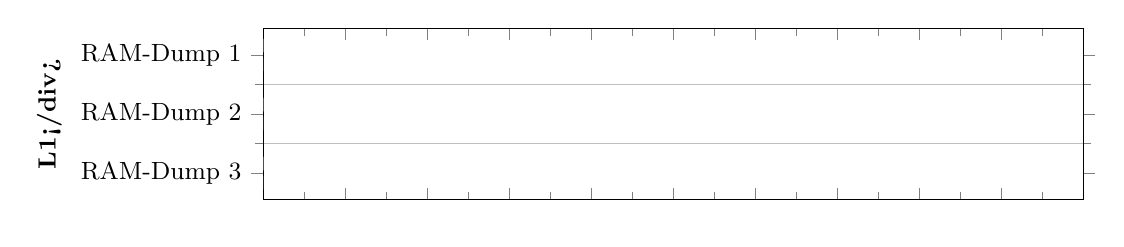
\begin{tikzpicture}
				\begin{axis}[
					xbar,
					width=12cm, 
					height=3cm, 
					ylabel style={align=center}, ylabel=\textbf{L1</div>},
					y=0.75cm,
					symbolic y coords={RAM-Dump 3, RAM-Dump 2, RAM-Dump 1},
					label style={font=\small},
					tick label style={font=\small},
					ytick=data,
					xticklabels={,,},
					xmin = 0,
					xmax = 5,
					nodes near coords, 
					nodes near coords align={horizontal},
					nodes near coords style={font=\tiny},
					nodes near coords={\pgfmathfloatifflags{\pgfplotspointmeta}{0}{}{\pgfmathprintnumber{\pgfplotspointmeta}}},
					bar width=.17cm,
					enlarge y limits={abs=2*\pgfplotbarwidth},
					scaled x ticks=false,
					legend style={
						at={(0.5,-0.1)},
						anchor=north
					},
					legend columns=3,
					yminorgrids = true,minor tick num=1
					]
					\addplot coordinates {
						(0,RAM-Dump 3)  (0,RAM-Dump 2) (0,RAM-Dump 1)
					};
					\addplot coordinates {
						(0,RAM-Dump 3)  (0,RAM-Dump 2) (0,RAM-Dump 1)
					};
				\end{axis}
			\end{tikzpicture}
			\\[-7pt]
			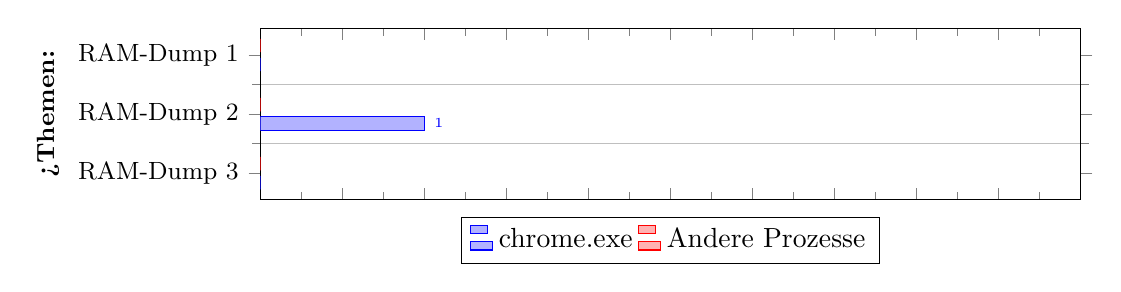
\begin{tikzpicture}
				\begin{axis}[
					xbar,
					width=12cm, 
					height=3cm, 
					ylabel style={align=center}, ylabel=\textbf{>Themen:},
					y=0.75cm,
					symbolic y coords={RAM-Dump 3, RAM-Dump 2, RAM-Dump 1},
					label style={font=\small},
					tick label style={font=\small},
					ytick=data,
					xticklabels={,,},
					xmin = 0,
					xmax = 5,
					nodes near coords, 
					nodes near coords align={horizontal},
					nodes near coords style={font=\tiny},
					nodes near coords={\pgfmathfloatifflags{\pgfplotspointmeta}{0}{}{\pgfmathprintnumber{\pgfplotspointmeta}}},
					bar width=.17cm,
					enlarge y limits={abs=2*\pgfplotbarwidth},
					scaled x ticks=false,
					legend style={
						at={(0.5,-0.1)},
						anchor=north
					},
					legend columns=3,
					yminorgrids = true,minor tick num=1
					]
					\addplot coordinates {
						(0,RAM-Dump 3)  (1,RAM-Dump 2) (0,RAM-Dump 1)
					};
					\addplot coordinates {
						(0,RAM-Dump 3)  (0,RAM-Dump 2) (0,RAM-Dump 1)
					};
					\legend{chrome.exe, Andere Prozesse}
				\end{axis}
			\end{tikzpicture}
		\end{tabular}
	}
	\caption{Anzahl gefundener HTML-Fragmente im Chrome RAM}
	\label{chart:chrome-volatility-htmls}
\end{table}

Das Volatility-Plugin lieferte hierbei neben dem Treffer noch die PID (7012 in diesem Fall) des Prozesses, in welchem der String gefunden wurde, sowie die virtuelle Adresse, an welchem das Fragment gefunden wurde (0xa6c018187e1). Mit dieser Information wurde dann zunächst der Befehl \texttt{python3 vol.py -f DUMP\_FILE windows.memmap --pid 7012} ausgeführt, um das Memory-Mapping des Prozesses zu erhalten, also die Zuordnung der virtuellen zu den physischen Adressen des Prozesses, sowie deren Offset im Memory-Dump-File. Nachfolgend ist ein Ausschnitt der Ausgabe des Befehls zu sehen:

\begin{table}[h!]
	\centering
	\begin{tabular}{llllll}
		Virtual                              & Physical                          & Size                          & Offset in File                   & File output                     &  \\
		0xa6c01817000                        & 0xc4efc000                        & 0x1000                        & 0x105d000                        & Disabled                        &  \\
		{\color[HTML]{FE0000} 0xa6c01818000} & {\color[HTML]{FE0000} 0xd2dfb000} & {\color[HTML]{FE0000} 0x1000} & {\color[HTML]{FE0000} 0x105e000} & {\color[HTML]{FE0000} Disabled} &  \\
		0xa6c01819000                        & 0xd50fa000                        & 0x1000                        & 0x105f000                        & Disabled                        & 
	\end{tabular}
\end{table}

In der Farbe rot ist hervorgehoben, dass die virtuelle Adresse 0xa6c01818000 auf die physikalische Adresse 0xd2dfb000 gemapped ist und der Offset im memory-file 0x105e000 entspricht. Mithilfe dieser Adressen konnte dann die tatsächliche Position des String im memory-file errechnet werden. Diese betrug somit 0x105e7e1. Anschließend wurde der gesamte Prozess mithilfe von Volatility gedumped und dieses memory-dump-file wurde anschließend in den Hex-Editor HxD geladen. Dort wurde dann genau an dem errechneten Offset nach dem String gesucht und konnte genau dort auch gefunden werden, was auch in \autoref{pic:ChromeStringThemen} zu sehen ist.
%TODO Evtl doch des andere Bild...

\begin{figure}[h!]
	\centering
	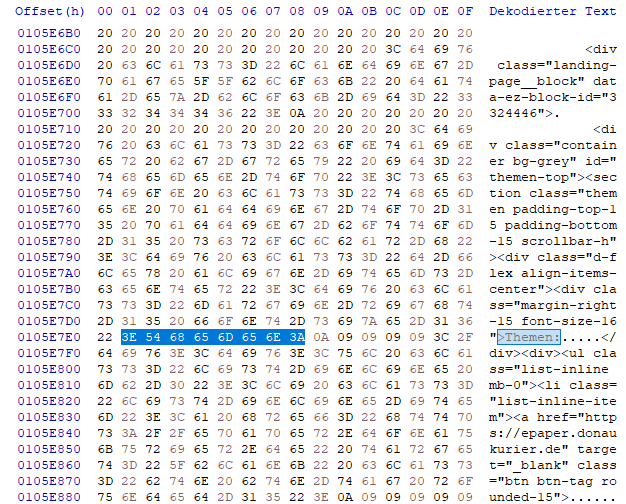
\includegraphics[width=0.75\textwidth]{bilder/HxDChromeStringThemen.png}
	\caption{Ausschnitt aus dem Memory-Dump-File an der Stelle des gefundenen Strings}
	\label{pic:ChromeStringThemen}
\end{figure} 

Daraufhin wurde weitergehend versucht zu analysieren, ob nur ein Teil der Website im RAM verfügbar ist, oder ob die komplette Donaukurier-Website als HTML Artefakt im RAM vorhanden ist. Dafür wurde die Internetseite donaukurier.de nochmals aufgerufen, heruntergeladen und der Beginn sowie das Ende der HTML-Datei analysiert. Nachfolgend sind die ersten sowie letzten Wörter der HTML-Datei zu sehen:\\

\begin{minted}[autogobble=true,frame=single,label=Beginn und Ende der Donaukurier-Website]{html}
	<!DOCTYPE html>
	<html lang="de">
	<head>
	
	<! ... >
	
	    </script>
	</body>
	</html>
\end{minted}

Davon ausgehend wurde in HxD zuerst nach dem String \glqq{}<!DOCTYPE html>\grqq{} und anschließend nach \glqq{}</html>\grqq{} gesucht. Beide Strings wurden mehrfach in dem Memory-Dump gefunden. Da jedoch keine weiteren Website-typischen Strings mehr durch Yarascan identifiziert werden konnten, wurden die übrigen String-Treffer nicht mehr weiter analysiert.\\
Da bei der Suche des Strings mehr als einen Treffer gab, wurde genau der String ausgewählt, welcher einen niedrigeren Offset als 0x105e7e1 aufweist. In diesem Fall war das der Treffer bei dem Offset von 105201b, was auch in \autoref{pic:ChromeBeginDonaukurier} zu sehen ist (markierter Teil). Dabei ist deutlich zu erkennen, dass die Website hier beginnt, da alles Nachfolgende mit dem Beginn der heruntergeladenen Website übereinstimmt und davor nichts im RAM gespeichert wurde.

\begin{figure}[h!]
	\centering
	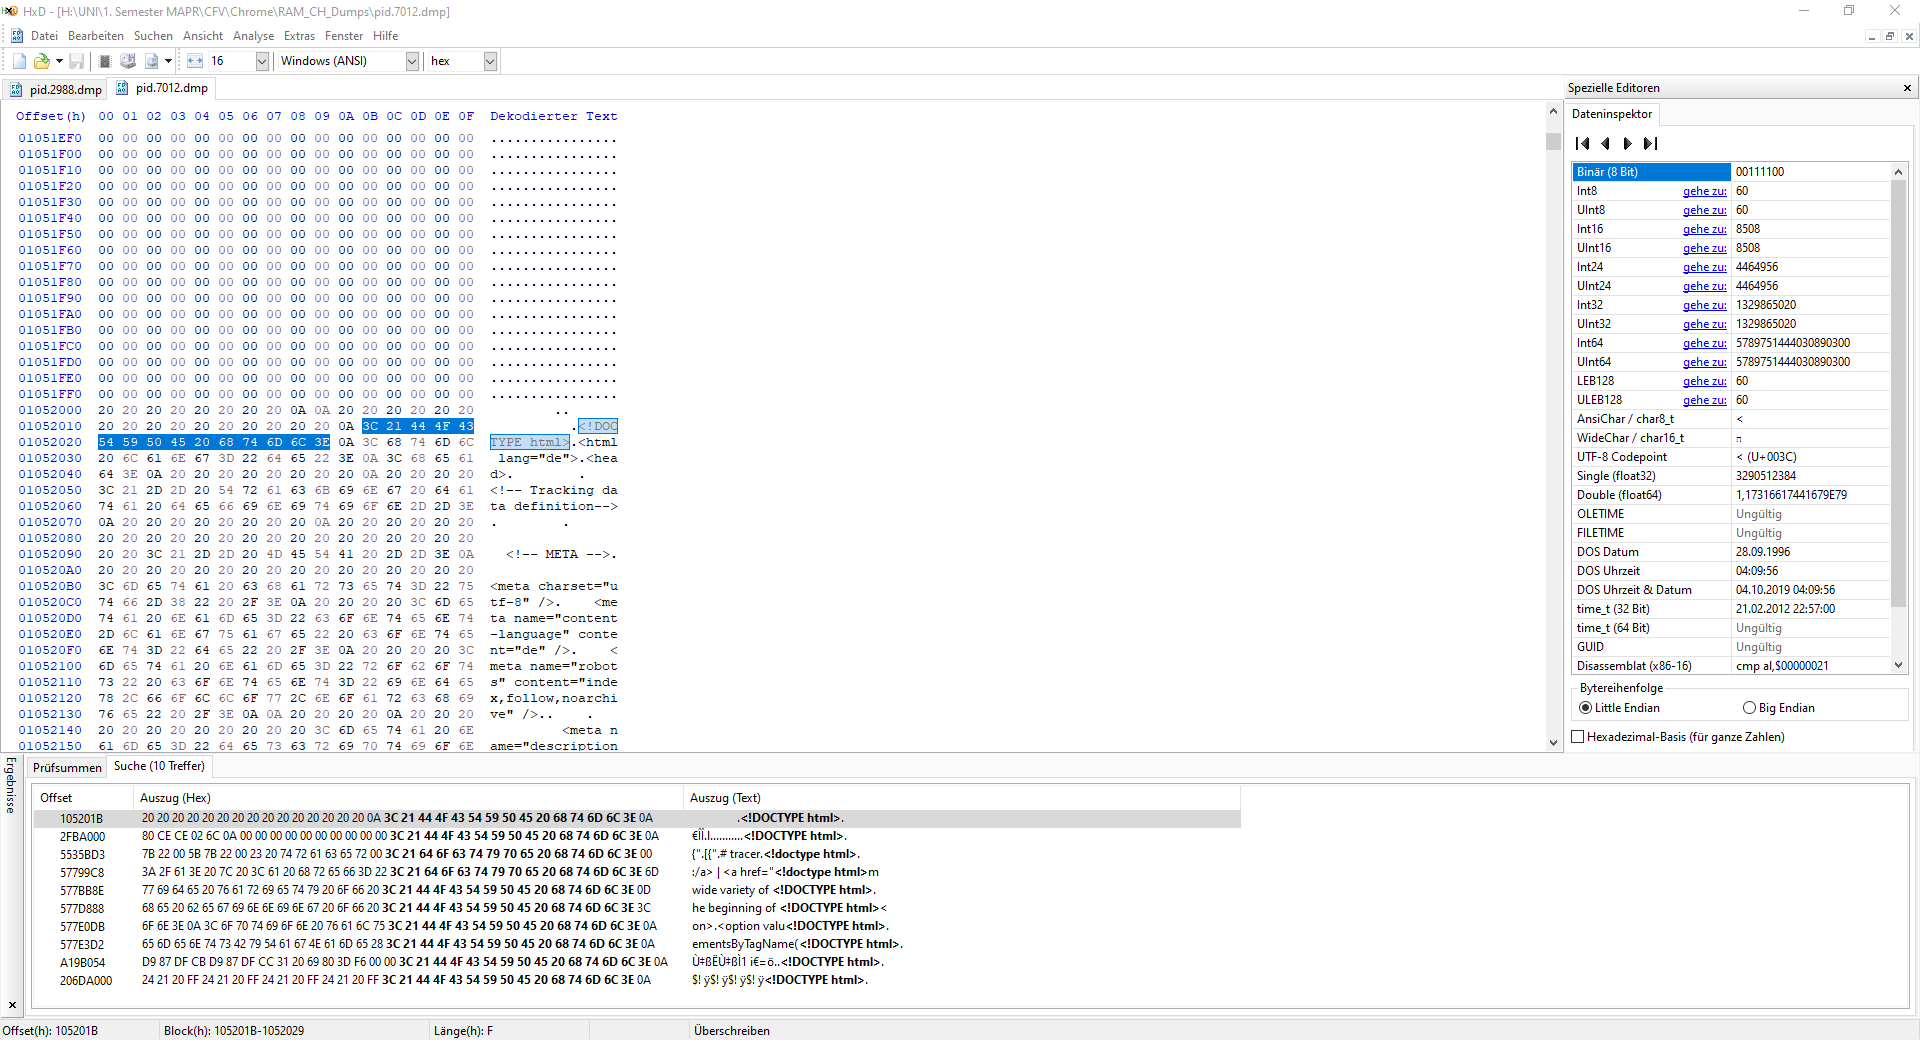
\includegraphics[width=\textwidth]{bilder/HxDChrome1.png}
	\caption{Beginn der Donaukurier-Website}
	\label{pic:ChromeBeginDonaukurier}
\end{figure} 

Gleiches wurde mit dem Ende der HTML-Datei durchgeführt. \autoref{pic:ChromeEndDonaukurier} zeigt einen Screenshot mit dem relevanten String-Treffer, welcher das Ende der Website donaukurier.de darstellt.

\begin{figure}[h!]
	\centering
	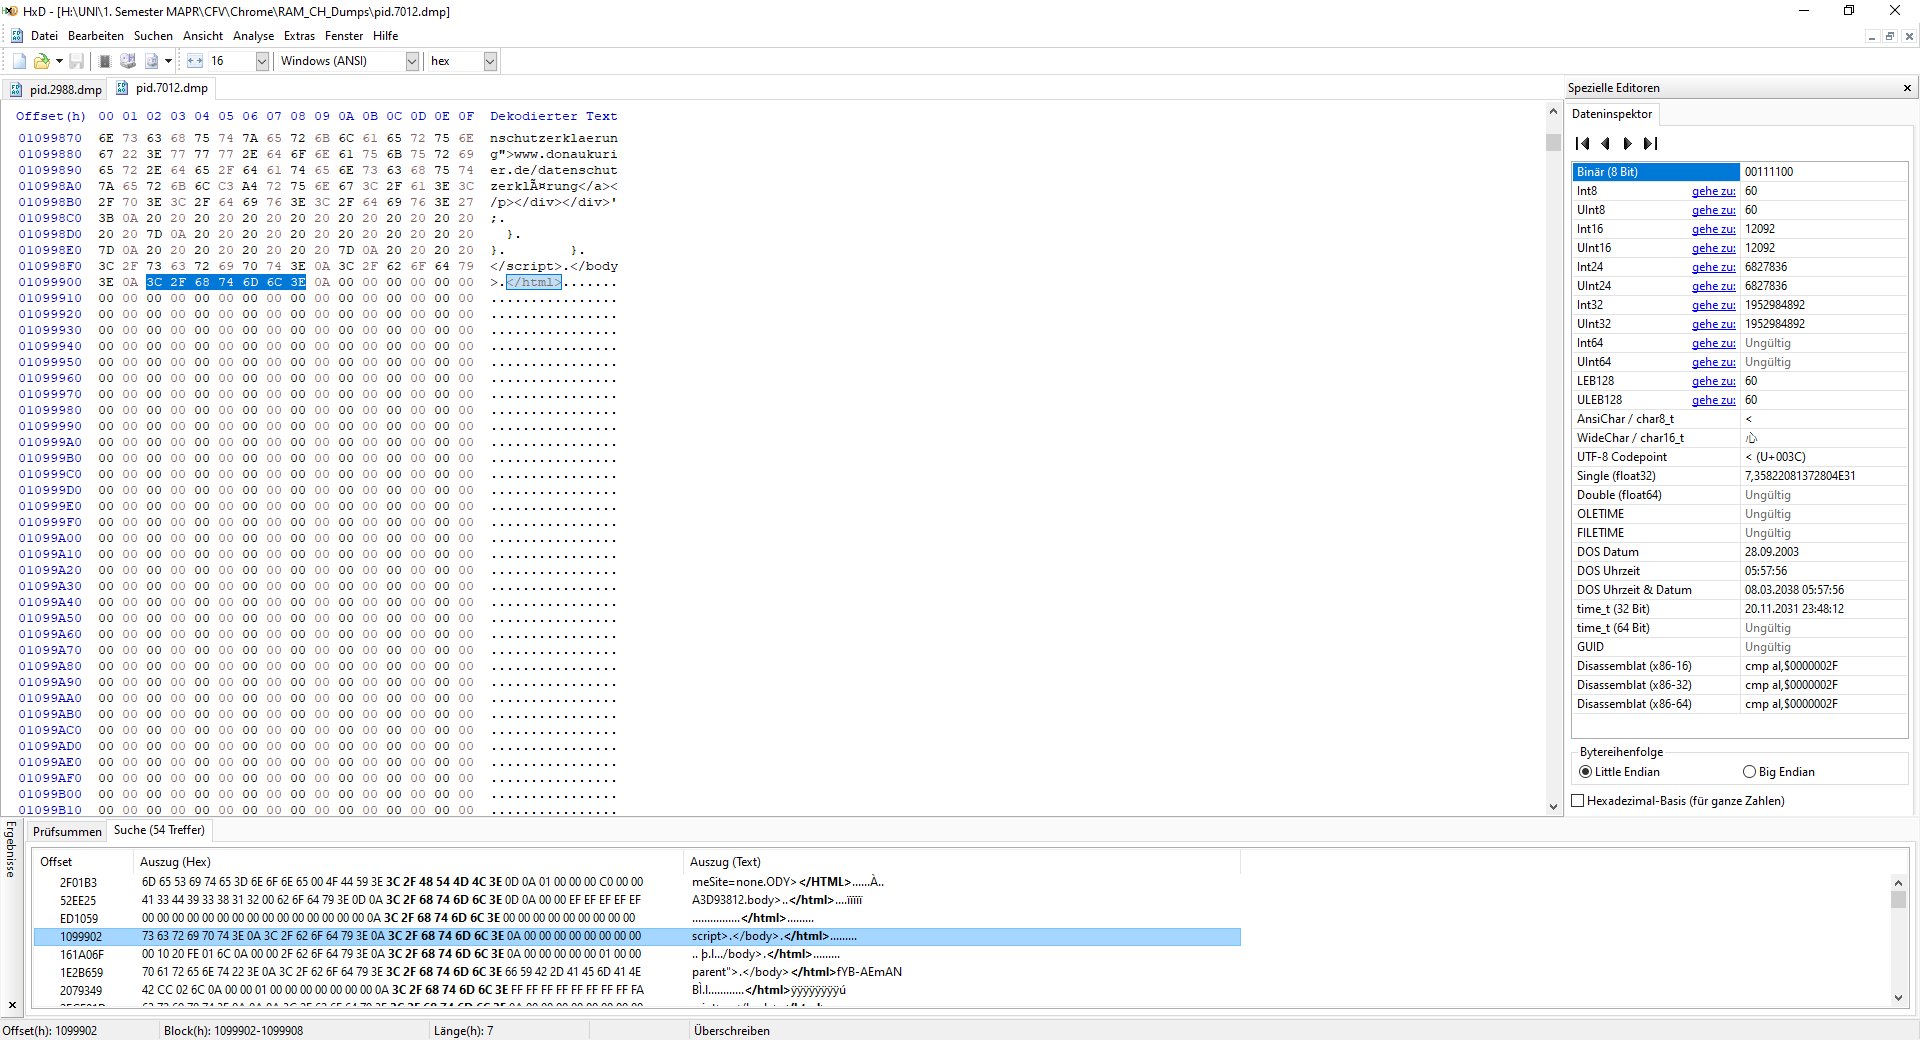
\includegraphics[width=\textwidth]{bilder/HxDChrome3.png}
	\caption{Ende der Donaukurier-Website}
	\label{pic:ChromeEndDonaukurier}
\end{figure} 

Anschließend wurde alles, was sich zwischen dem gefundenem Anfang und Ende befindet, als Text kopiert und in eine html-Datei gespeichert. Ein detaillierter Vergleich dieses extrahierten Artefakts mit der heruntergeladenen Datei lieferte das Ergebnis, dass die komplette Website rekonstruiert werden kann, die Websiten sich nur in den neuesten Artikeln und Überschriften unterschieden. Übriges war zu 100\% identisch. \\
Zusammenfassend konnte somit die Website \glqq{}donaukurier.de\grqq{} im zweiten Memory-Dump komplett aus dem RAM extrahiert und rekonstruiert werden.

\paragraph*{Yara-Regel \glqq{}Suchbegriffe\grqq{}}\label{chap:ergebnisse-chrome-uncommon-volatility-suchbegriffe}

Wie in \autoref{chart:chrome-volatility-keywords} dargestellt, wurden die Suchbegriffe \glqq{}pfaffenhofen\grqq{}, \glqq{}nanoradar\grqq{}, \glqq{}mooserliesl\grqq{} und \glqq{}mallofamerica\grqq{} ausschließlich bei dem noch geöffnetem Chrome-Browser nach dem Browsing-Szenario (zweiter RAM Dump) gefunden. Es wurden dabei alle Suchbegriffe bis auf einen einzigen in Speicherbereichen des Chrome-Browsers gefunden. Am häufigsten konnte der Suchbegriff \glqq{}pfaffenhofen\grqq{} mit 1922 Treffern identifiziert werden. Am seltensten war das der Fall bei dem Begriff \glqq{}mooserliesl\grqq{} mit nur 281 Suchtreffern. \\
Der eine Treffer bei der Suchphrase \glqq{}mallofamerica\grqq{} war im Speicher eines Prozesses mit dem Namen \textit{MemCompression}, was anhand der PID 1828 festgestellt wurde. Dieser Prozess ist dafür zuständig, dass Windows einen Teil des Arbeitsspeichers komprimiert speichert, was zwar zusätzliche CPU-Ressourcen beansprucht, dafür jedoch deutlich schneller ist, als den Hauptspeicher in das pagefile auszulagern \cite{MemCompressionWebsite}. Daher kann es sein, dass ein Teil des RAMs, in welchem der Suchbegriff vorhanden war, komprimiert wurde und folglich dieser Prozess diesen Begriff beinhaltete.

\begin{table}[h!]
	\resizebox{\linewidth}{!}{
		\begin{tabular}{l}	
			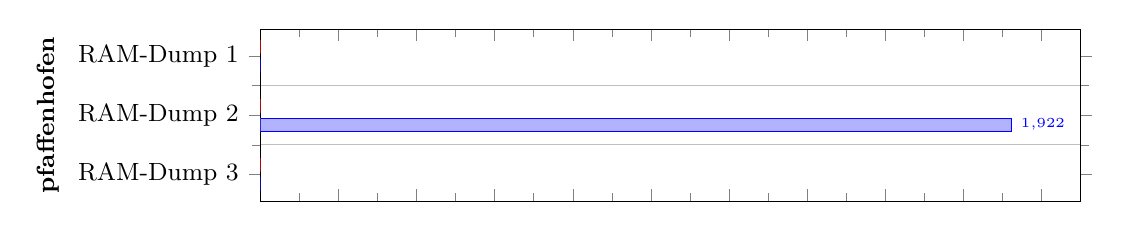
\begin{tikzpicture}
				\begin{axis}[
					xbar,
					width=12cm, 
					height=3cm, 
					ylabel style={align=center}, ylabel=\textbf{pfaffenhofen},
					y=0.75cm,
					symbolic y coords={RAM-Dump 3, RAM-Dump 2, RAM-Dump 1},
					label style={font=\small},
					tick label style={font=\small},
					ytick=data,
					xticklabels={,,},
					xmin = 0,
					xmax = 2100,
					nodes near coords, 
					nodes near coords align={horizontal},
					nodes near coords style={font=\tiny},
					nodes near coords={\pgfmathfloatifflags{\pgfplotspointmeta}{0}{}{\pgfmathprintnumber{\pgfplotspointmeta}}},
					bar width=.17cm,
					enlarge y limits={abs=2*\pgfplotbarwidth},
					scaled x ticks=false,
					legend style={
						at={(0.5,-0.1)},
						anchor=north
					},
					legend columns=3,
					yminorgrids = true,minor tick num=1
					]
					\addplot coordinates {
						(0,RAM-Dump 3) (1922,RAM-Dump 2) (0,RAM-Dump 1)
					};
					\addplot coordinates {
						(0,RAM-Dump 3) (0,RAM-Dump 2) (0,RAM-Dump 1)
					};
				\end{axis}
			\end{tikzpicture}
			\\[-7pt]
			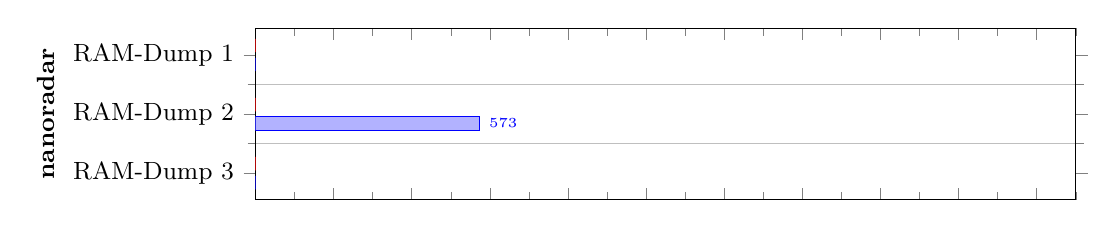
\begin{tikzpicture}
				\begin{axis}[
					xbar,
					width=12cm, 
					height=3cm, 
					ylabel style={align=center}, ylabel=\textbf{nanoradar},
					y=0.75cm,
					symbolic y coords={RAM-Dump 3, RAM-Dump 2, RAM-Dump 1},
					label style={font=\small},
					tick label style={font=\small},
					ytick=data,
					xticklabels={,,},
					xmin = 0,
					xmax = 2100,
					nodes near coords, 
					nodes near coords align={horizontal},
					nodes near coords style={font=\tiny},
					nodes near coords={\pgfmathfloatifflags{\pgfplotspointmeta}{0}{}{\pgfmathprintnumber{\pgfplotspointmeta}}},
					bar width=.17cm,
					enlarge y limits={abs=2*\pgfplotbarwidth},
					scaled x ticks=false,
					legend style={
						at={(0.5,-0.1)},
						anchor=north
					},
					legend columns=3,
					yminorgrids = true,minor tick num=1
					]
					\addplot coordinates {
						(0,RAM-Dump 3)  (573,RAM-Dump 2) (0,RAM-Dump 1)
					};
					\addplot coordinates {
						(0,RAM-Dump 3)  (0,RAM-Dump 2) (0,RAM-Dump 1)
					};
				\end{axis}
			\end{tikzpicture}
			\\[-7pt]
			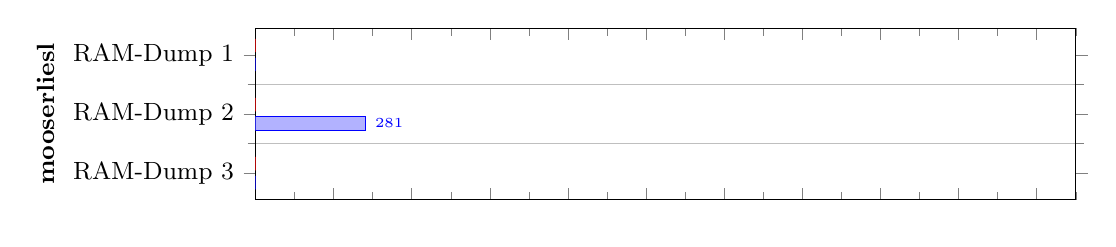
\begin{tikzpicture}
				\begin{axis}[
					xbar,
					width=12cm, 
					height=3cm, 
					ylabel style={align=center}, ylabel=\textbf{mooserliesl},
					y=0.75cm,
					symbolic y coords={RAM-Dump 3, RAM-Dump 2, RAM-Dump 1},
					label style={font=\small},
					tick label style={font=\small},
					ytick=data,
					xticklabels={,,},
					xmin = 0,
					xmax = 2100,
					nodes near coords, 
					nodes near coords align={horizontal},
					nodes near coords style={font=\tiny},
					nodes near coords={\pgfmathfloatifflags{\pgfplotspointmeta}{0}{}{\pgfmathprintnumber{\pgfplotspointmeta}}},
					bar width=.17cm,
					enlarge y limits={abs=2*\pgfplotbarwidth},
					scaled x ticks=false,
					legend style={
						at={(0.5,-0.1)},
						anchor=north
					},
					legend columns=3,
					yminorgrids = true,minor tick num=1
					]
					\addplot coordinates {
						(0,RAM-Dump 3)  (281,RAM-Dump 2) (0,RAM-Dump 1)
					};
					\addplot coordinates {
						(0,RAM-Dump 3)  (0,RAM-Dump 2) (0,RAM-Dump 1)
					};
				\end{axis}
			\end{tikzpicture}
			\\[-7pt]
			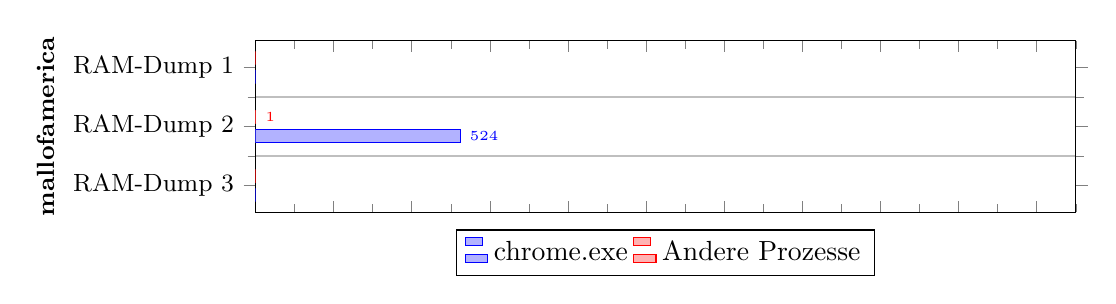
\begin{tikzpicture}
				\begin{axis}[
					xbar,
					width=12cm, 
					height=3cm, 
					ylabel style={align=center}, ylabel=\textbf{mallofamerica},
					y=0.75cm,
					symbolic y coords={RAM-Dump 3, RAM-Dump 2, RAM-Dump 1},
					label style={font=\small},
					tick label style={font=\small},
					ytick=data,
					xticklabels={,,},
					xmin = 0,
					xmax = 2100,
					nodes near coords, 
					nodes near coords align={horizontal},
					nodes near coords style={font=\tiny},
					nodes near coords={\pgfmathfloatifflags{\pgfplotspointmeta}{0}{}{\pgfmathprintnumber{\pgfplotspointmeta}}},
					bar width=.17cm,
					enlarge y limits={abs=2*\pgfplotbarwidth},
					scaled x ticks=false,
					legend style={
						at={(0.5,-0.1)},
						anchor=north
					},
					legend columns=3,
					yminorgrids = true,minor tick num=1
					]
					\addplot coordinates {
						(0,RAM-Dump 3)  (524,RAM-Dump 2) (0,RAM-Dump 1)
					};
					\addplot coordinates {
						(0,RAM-Dump 3)  (1,RAM-Dump 2) (0,RAM-Dump 1)
					};
					\legend{chrome.exe, Andere Prozesse}
				\end{axis}
			\end{tikzpicture}
		\end{tabular}
	}
	\caption{Anzahl gefundener Suchbegriffe im Chrome RAM}
	\label{chart:chrome-volatility-keywords}
\end{table}

\paragraph*{Yara-Regel \glqq{}URLs\grqq{}}\label{chap:ergebnisse-chrome-uncommon-volatility-urls}

\autoref{chart:chrome-volatility-urls} zeigt, dass in den RAM-Dumps alle Suchbegriffe identifiziert werden konnten. Im ersten Speicherabbild wurden dabei keine URLs gefunden, im zweiten am meisten und im dritten, also nach Beenden des Browsers, konnten auch noch 5 URLs identifiziert werden. Dabei waren es bei der URL \glqq{}donaukurier.com\grqq{} am meisten Suchtreffer mit insgesammt 8157 Treffern, 10 davon waren nicht im Speicher von Chrome-Prozessen zu finden. Zwei davon waren im Prozess \textit{MemCompression}, die restlichen acht wurden im Prozess mit der PID 3760 identifiziert, was in diesem Fall der sihost.exe war. Dieses Programm entspricht dem \textit{Shell Infrastructure Host}, welcher die Grafikbenutzeroberflächer erstellt und verwaltet, wie beispielsweise Desktop-Hintergründe, Popup-Benachrichtigungen und Taskleisten \cite{SiHostWebsite}. Im Prozessbereich dieses Programms befanden sich auch die 5 Treffer aus dem dritten RAM-Dump.

\begin{table}[h!]
	\resizebox{\linewidth}{!}{
		\begin{tabular}{l}	
			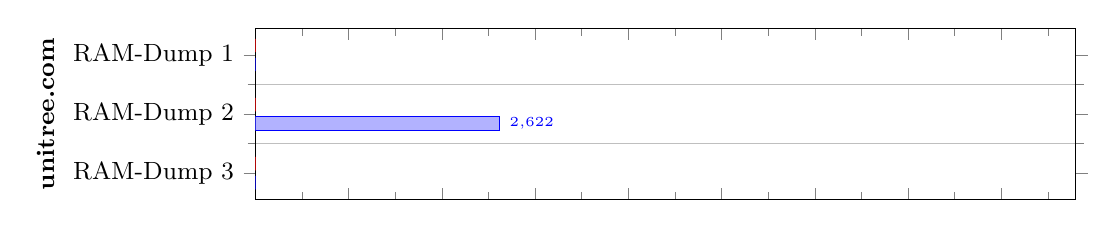
\begin{tikzpicture}
				\begin{axis}[
					xbar,
					width=12cm, 
					height=3cm, 
					ylabel style={align=center}, ylabel=\textbf{unitree.com},
					y=0.75cm,
					symbolic y coords={RAM-Dump 3, RAM-Dump 2, RAM-Dump 1},
					label style={font=\small},
					tick label style={font=\small},
					ytick=data,
					xticklabels={,,},
					xmin = 0,
					xmax = 8800,
					nodes near coords, 
					nodes near coords align={horizontal},
					nodes near coords style={font=\tiny},
					nodes near coords={\pgfmathfloatifflags{\pgfplotspointmeta}{0}{}{\pgfmathprintnumber{\pgfplotspointmeta}}},
					bar width=.17cm,
					enlarge y limits={abs=2*\pgfplotbarwidth},
					scaled x ticks=false,
					legend style={
						at={(0.5,-0.1)},
						anchor=north
					},
					legend columns=3,
					yminorgrids = true,minor tick num=1
					]
					\addplot coordinates {
						(0,RAM-Dump 3) (2622,RAM-Dump 2) (0,RAM-Dump 1)
					};
					\addplot coordinates {
						(0,RAM-Dump 3) (0,RAM-Dump 2) (0,RAM-Dump 1)
					};
				\end{axis}
			\end{tikzpicture}
			\\[-7pt]
			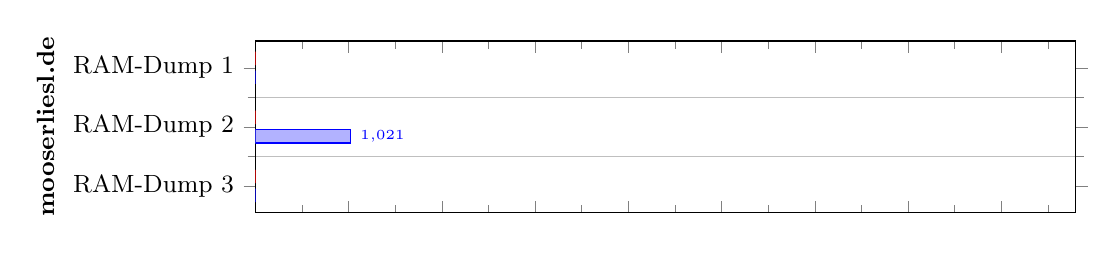
\begin{tikzpicture}
				\begin{axis}[
					xbar,
					width=12cm, 
					height=3cm, 
					ylabel style={align=center}, ylabel=\textbf{mooserliesl.de},
					y=0.75cm,
					symbolic y coords={RAM-Dump 3, RAM-Dump 2, RAM-Dump 1},
					label style={font=\small},
					tick label style={font=\small},
					ytick=data,
					xticklabels={,,},
					xmin = 0,
					xmax = 8800,
					nodes near coords, 
					nodes near coords align={horizontal},
					nodes near coords style={font=\tiny},
					nodes near coords={\pgfmathfloatifflags{\pgfplotspointmeta}{0}{}{\pgfmathprintnumber{\pgfplotspointmeta}}},
					bar width=.17cm,
					enlarge y limits={abs=2*\pgfplotbarwidth},
					scaled x ticks=false,
					legend style={
						at={(0.5,-0.1)},
						anchor=north
					},
					legend columns=3,
					yminorgrids = true,minor tick num=1
					]
					\addplot coordinates {
						(0,RAM-Dump 3) (1021,RAM-Dump 2) (0,RAM-Dump 1)
					};
					\addplot coordinates {
						(0,RAM-Dump 3) (0,RAM-Dump 2) (0,RAM-Dump 1)
					};
				\end{axis}
			\end{tikzpicture}	
			\\[-7pt]
			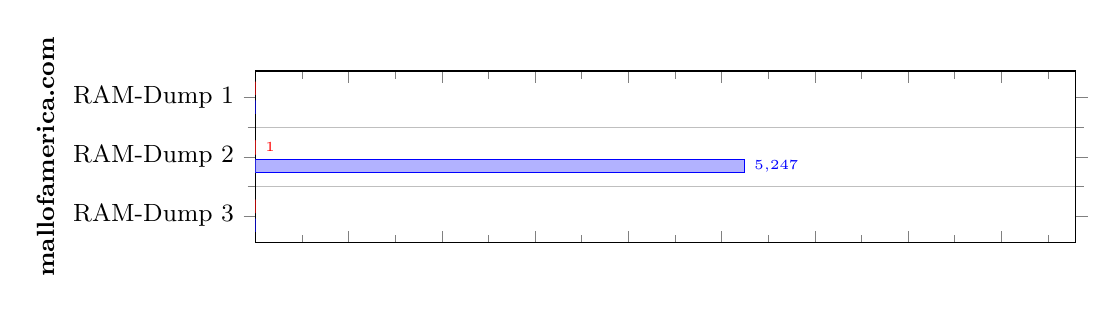
\begin{tikzpicture}
				\begin{axis}[
					xbar,
					width=12cm, 
					height=3cm, 
					ylabel style={align=center}, ylabel=\textbf{mallofamerica.com},
					y=0.75cm,
					symbolic y coords={RAM-Dump 3, RAM-Dump 2, RAM-Dump 1},
					label style={font=\small},
					tick label style={font=\small},
					ytick=data,
					xticklabels={,,},
					xmin = 0,
					xmax = 8800,
					nodes near coords, 
					nodes near coords align={horizontal},
					nodes near coords style={font=\tiny},
					nodes near coords={\pgfmathfloatifflags{\pgfplotspointmeta}{0}{}{\pgfmathprintnumber{\pgfplotspointmeta}}},
					bar width=.17cm,
					enlarge y limits={abs=2*\pgfplotbarwidth},
					scaled x ticks=false,
					legend style={
						at={(0.5,-0.1)},
						anchor=north
					},
					legend columns=3,
					yminorgrids = true,minor tick num=1
					]
					\addplot coordinates {
						(0,RAM-Dump 3) (5247,RAM-Dump 2) (0,RAM-Dump 1)
					};
					\addplot coordinates {
						(0,RAM-Dump 3) (1,RAM-Dump 2) (0,RAM-Dump 1)
					};
				\end{axis}
			\end{tikzpicture}
			\\[-7pt]
			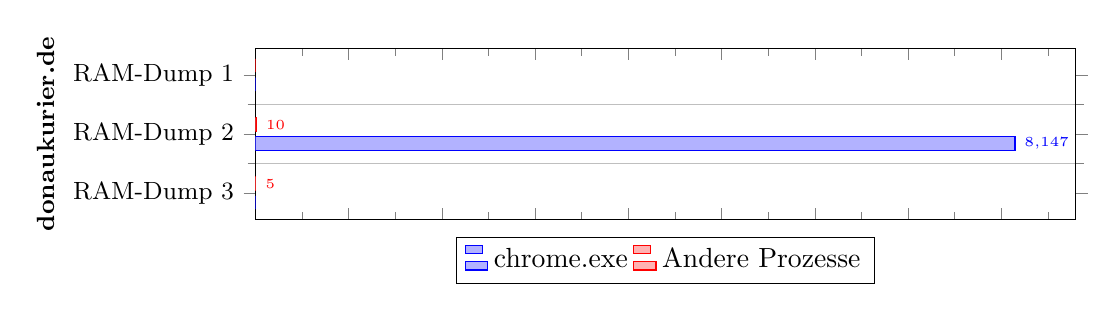
\begin{tikzpicture}
				\begin{axis}[
					xbar,
					width=12cm, 
					height=3cm, 
					ylabel style={align=center}, ylabel=\textbf{donaukurier.de},
					y=0.75cm,
					symbolic y coords={RAM-Dump 3, RAM-Dump 2, RAM-Dump 1},
					label style={font=\small},
					tick label style={font=\small},
					ytick=data,
					xticklabels={,,},
					xmin = 0,
					xmax = 8800,
					nodes near coords, 
					nodes near coords align={horizontal},
					nodes near coords style={font=\tiny},
					nodes near coords={\pgfmathfloatifflags{\pgfplotspointmeta}{0}{}{\pgfmathprintnumber{\pgfplotspointmeta}}},
					bar width=.17cm,
					enlarge y limits={abs=2*\pgfplotbarwidth},
					scaled x ticks=false,
					legend style={
						at={(0.5,-0.1)},
						anchor=north
					},
					legend columns=3,
					yminorgrids = true,minor tick num=1
					]
					\addplot coordinates {
						(0,RAM-Dump 3) (8147,RAM-Dump 2) (0,RAM-Dump 1)
					};
					\addplot coordinates {
						(5,RAM-Dump 3) (10,RAM-Dump 2) (0,RAM-Dump 1)
					};
					\legend{chrome.exe, Andere Prozesse}
				\end{axis}
			\end{tikzpicture}		
		\end{tabular}
	}
	\caption{Anzahl gefundener URLs im Chrome RAM}
	\label{chart:chrome-volatility-urls}
\end{table}

\paragraph*{Yara-Regel \glqq{}E-Mail\grqq{}}\label{chap:ergebnisse-chrome-uncommon-volatility-email}
Wie in \autoref{chart:chrome-volatility-mail} gezeigt, wurden sowohl nach dem Browsing Szenario bei geöffnetem Browser, als auch nach Schließen desselben E-Mail Artefakte gefunden. Darunter war die E-Mail-Adresse mit 172 Treffern, 8 davon außerhalb von Chrome-Prozessen, das häufigste Suchresultat. unter den acht externen Prozessen waren der \textit{Desktop Window Manager}, welcher für visuelle Effekte wie Desktop-Animationen und halbtransparente Fenster verantwortlich ist \cite{dwmWebsite}, explorer.exe, sihost.exe und weiteren Windows-Prozessen. Da dies aber meist Prozesse waren, welche grafische Aktionen durchführten, wurden diese nicht weiter analysiert.\\
Die beiden Studenten-Mailadressen, an welche die Mail versendet wurden, waren mit 121 bzw. 97 Suchtreffern in Chrome-Prozessen vertreten. Der Mailtext war mit 136 Artefakten mehr als doppelt so oft im RAM zu finden als der Betrefftext. Im dritten RAM-Dump wurde dann noch die E-Mail-Adresse im Prozess \textit{explorer.exe} gefunden.\\
Grundsätzlich wurden bei dieser Yara-Regel wenige Artefakte identifiziert im Vergleich zu den URLs beispielsweise.


\begin{table}[h!]
	\resizebox{\linewidth}{!}{
		\begin{tabular}{r}	
			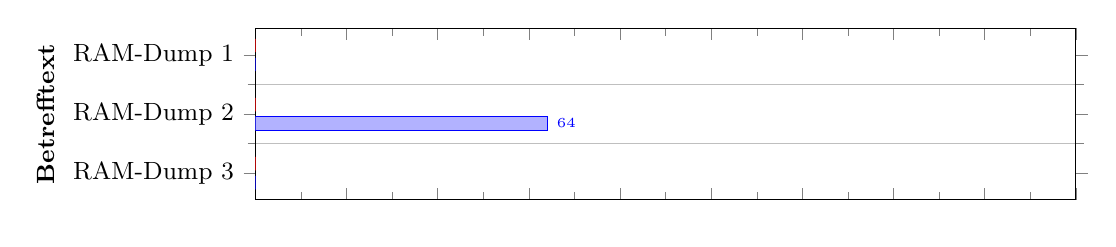
\begin{tikzpicture}
				\begin{axis}[
					xbar,
					width=12cm, 
					height=3cm, 
					ylabel style={align=center}, ylabel=\textbf{Betrefftext},
					y=0.75cm,
					symbolic y coords={RAM-Dump 3, RAM-Dump 2, RAM-Dump 1},
					label style={font=\small},
					tick label style={font=\small},
					ytick=data,
					xticklabels={,,},
					xmin = 0,
					xmax = 180,
					nodes near coords, 
					nodes near coords align={horizontal},
					nodes near coords style={font=\tiny},
					nodes near coords={\pgfmathfloatifflags{\pgfplotspointmeta}{0}{}{\pgfmathprintnumber{\pgfplotspointmeta}}},
					bar width=.17cm,
					enlarge y limits={abs=2*\pgfplotbarwidth},
					scaled x ticks=false,
					legend style={
						at={(0.5,-0.1)},
						anchor=north
					},
					legend columns=3,
					yminorgrids = true,minor tick num=1
					]
					\addplot coordinates {
						(0,RAM-Dump 3) (64,RAM-Dump 2) (0,RAM-Dump 1)
					};
					\addplot coordinates {
						(0,RAM-Dump 3) (0,RAM-Dump 2) (0,RAM-Dump 1)
					};
					%				\legend{firefox.exe, Andere Prozesse}
				\end{axis}
			\end{tikzpicture}
			\\[-7pt]
			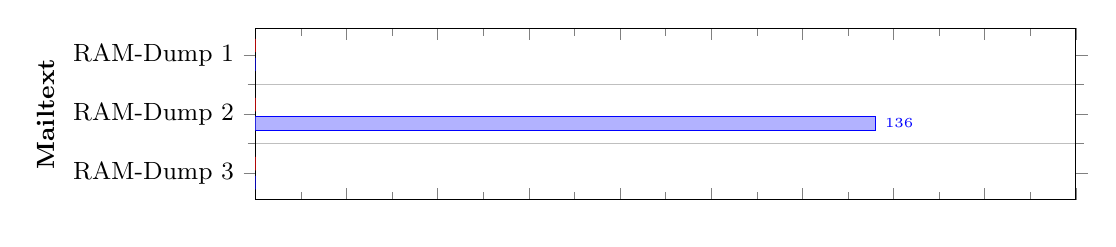
\begin{tikzpicture}
				\begin{axis}[
					xbar,
					width=12cm, 
					height=3cm, 
					ylabel style={align=center}, ylabel=\textbf{Mailtext},
					y=0.75cm,
					symbolic y coords={RAM-Dump 3, RAM-Dump 2, RAM-Dump 1},
					label style={font=\small},
					tick label style={font=\small},
					ytick=data,
					xticklabels={,,},
					xmin = 0,
					xmax = 180,
					nodes near coords, 
					nodes near coords align={horizontal},
					nodes near coords style={font=\tiny},
					nodes near coords={\pgfmathfloatifflags{\pgfplotspointmeta}{0}{}{\pgfmathprintnumber{\pgfplotspointmeta}}},
					bar width=.17cm,
					enlarge y limits={abs=2*\pgfplotbarwidth},
					scaled x ticks=false,
					legend style={
						at={(0.5,-0.1)},
						anchor=north
					},
					legend columns=3,
					yminorgrids = true,minor tick num=1
					]
					\addplot coordinates {
						(0,RAM-Dump 3) (136,RAM-Dump 2) (0,RAM-Dump 1)
					};
					\addplot coordinates {
						(0,RAM-Dump 3) (0,RAM-Dump 2) (0,RAM-Dump 1)
					};
					%				\legend{firefox.exe, Andere Prozesse}
				\end{axis}
			\end{tikzpicture}	
			\\[-7pt]
			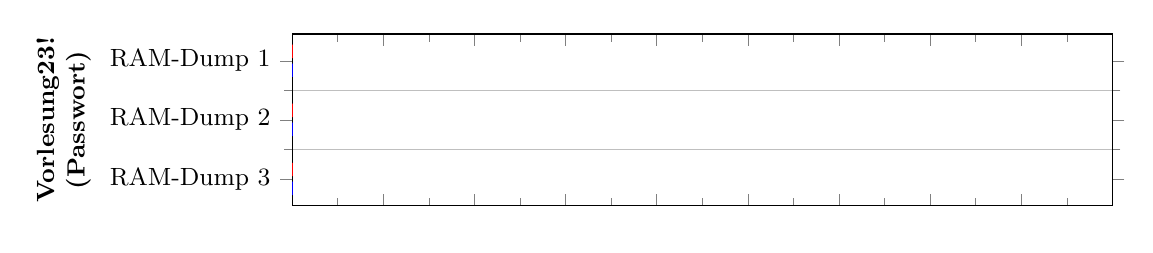
\begin{tikzpicture}
				\begin{axis}[
					xbar,
					width=12cm, 
					height=3cm, 
					ylabel style={align=center}, ylabel=\textbf{Vorlesung23!}\\\textbf{(Passwort)},
					y=0.75cm,
					symbolic y coords={RAM-Dump 3, RAM-Dump 2, RAM-Dump 1},
					label style={font=\small},
					tick label style={font=\small},
					ytick=data,
					xticklabels={,,},
					xmin = 0,
					xmax = 180,
					nodes near coords, 
					nodes near coords align={horizontal},
					nodes near coords style={font=\tiny},
					nodes near coords={\pgfmathfloatifflags{\pgfplotspointmeta}{0}{}{\pgfmathprintnumber{\pgfplotspointmeta}}},
					bar width=.17cm,
					enlarge y limits={abs=2*\pgfplotbarwidth},
					scaled x ticks=false,
					legend style={
						at={(0.5,-0.1)},
						anchor=north
					},
					legend columns=3,
					yminorgrids = true,minor tick num=1
					]
					\addplot coordinates {
						(0,RAM-Dump 3) (0,RAM-Dump 2) (0,RAM-Dump 1)
					};
					\addplot coordinates {
						(0,RAM-Dump 3) (0,RAM-Dump 2) (0,RAM-Dump 1)
					};
					%				\legend{firefox.exe, Andere Prozesse}
				\end{axis}
			\end{tikzpicture}
			\\[-7pt]
			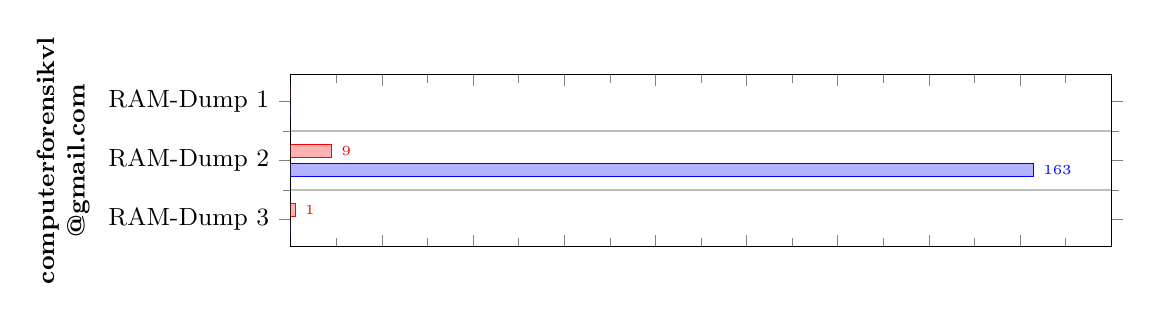
\begin{tikzpicture}
				\begin{axis}[
					xbar,
					width=12cm, 
					height=3cm, 
					ylabel style={align=center}, ylabel=\textbf{computerforensikvl}\\\textbf{@gmail.com},
					y=0.75cm,
					symbolic y coords={RAM-Dump 3, RAM-Dump 2, RAM-Dump 1},
					label style={font=\small},
					tick label style={font=\small},
					ytick=data,
					xticklabels={,,},
					xmin = 0,
					xmax = 180,
					nodes near coords, 
					nodes near coords align={horizontal},
					nodes near coords style={font=\tiny},
					nodes near coords={\pgfmathfloatifflags{\pgfplotspointmeta}{0}{}{\pgfmathprintnumber{\pgfplotspointmeta}}},
					bar width=.17cm,
					enlarge y limits={abs=2*\pgfplotbarwidth},
					scaled x ticks=false,
					legend style={
						at={(0.5,-0.1)},
						anchor=north
					},
					legend columns=3,
					yminorgrids = true,minor tick num=1
					]
					\addplot coordinates {
						(0,RAM-Dump 3) (163,RAM-Dump 2) (0,RAM-Dump 1)
					};
					\addplot coordinates {
						(1,RAM-Dump 3) (9,RAM-Dump 2) (0,RAM-Dump 1)
					};
					%				\legend{firefox.exe, Andere Prozesse}
				\end{axis}
			\end{tikzpicture}	
			\\[-7pt]
			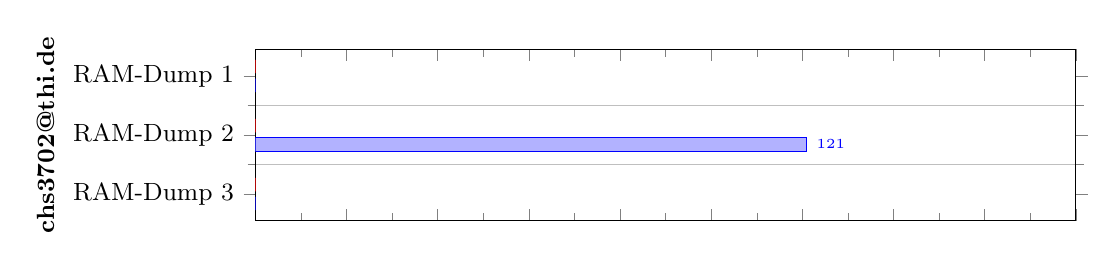
\begin{tikzpicture}
				\begin{axis}[
					xbar,
					width=12cm, 
					height=3cm, 
					ylabel style={align=center}, ylabel=\textbf{chs3702@thi.de},
					y=0.75cm,
					symbolic y coords={RAM-Dump 3, RAM-Dump 2, RAM-Dump 1},
					label style={font=\small},
					tick label style={font=\small},
					ytick=data,
					xticklabels={,,},
					xmin = 0,
					xmax = 180,
					nodes near coords, 
					nodes near coords align={horizontal},
					nodes near coords style={font=\tiny},
					nodes near coords={\pgfmathfloatifflags{\pgfplotspointmeta}{0}{}{\pgfmathprintnumber{\pgfplotspointmeta}}},
					bar width=.17cm,
					enlarge y limits={abs=2*\pgfplotbarwidth},
					scaled x ticks=false,
					legend style={
						at={(0.5,-0.1)},
						anchor=north
					},
					legend columns=3,
					yminorgrids = true,minor tick num=1
					]
					\addplot coordinates {
						(0,RAM-Dump 3) (121,RAM-Dump 2) (0,RAM-Dump 1)
					};
					\addplot coordinates {
						(0,RAM-Dump 3) (0,RAM-Dump 2) (0,RAM-Dump 1)
					};
					%				\legend{firefox.exe, Andere Prozesse}
				\end{axis}
			\end{tikzpicture}
			\\[-7pt]
			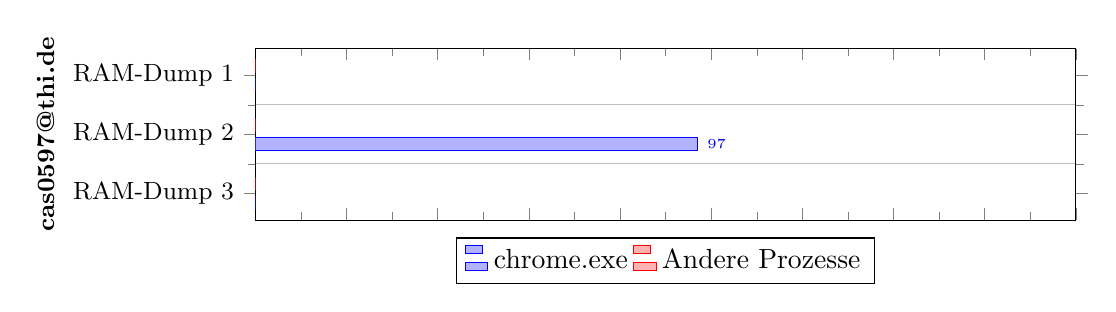
\begin{tikzpicture}
				\begin{axis}[
					xbar,
					width=12cm, 
					height=3cm, 
					ylabel style={align=center}, ylabel=\textbf{cas0597@thi.de},
					y=0.75cm,
					symbolic y coords={RAM-Dump 3, RAM-Dump 2, RAM-Dump 1},
					label style={font=\small},
					tick label style={font=\small},
					ytick=data,
					xticklabels={,,},
					xmin = 0,
					xmax = 180,
					nodes near coords, 
					nodes near coords align={horizontal},
					nodes near coords style={font=\tiny},
					nodes near coords={\pgfmathfloatifflags{\pgfplotspointmeta}{0}{}{\pgfmathprintnumber{\pgfplotspointmeta}}},
					bar width=.17cm,
					enlarge y limits={abs=2*\pgfplotbarwidth},
					scaled x ticks=false,
					legend style={
						at={(0.5,-0.1)},
						anchor=north
					},
					legend columns=3,
					yminorgrids = true,minor tick num=1
					]
					\addplot coordinates {
						(0,RAM-Dump 3) (97,RAM-Dump 2) (0,RAM-Dump 1)
					};
					\addplot coordinates {
						(0,RAM-Dump 3) (0,RAM-Dump 2) (0,RAM-Dump 1)
					};
					\legend{chrome.exe, Andere Prozesse}
				\end{axis}
			\end{tikzpicture}
			%	\begin{axis}[]
				%	\legend{Logfile 1, Logfile 2}
				%	\end{axis}
			
		\end{tabular}
	}
	\caption{Anzahl gefundener E-Mail Artefakte im Chrome RAM}
	\label{chart:chrome-volatility-mail}
\end{table}

\paragraph{Yara-Regel \glqq{}DK-Logo\grqq{}}\label{chap:ergebnisse-chrome-uncommon-volatility-dklogo}

Bei der letzten Yara-Regel zeigt \autoref{chart:chrome-volatility-image} die Ergebnisse, in welchem RAM-Dump und wie oft das Donaukurier Logo im RAM identifiziert werden konnte. Zu sehen ist, dass dies nur im zweiten Speicherabbild der Fall war und insgesamt 3 mal dort in einem Chrome-Prozess zu finden war.

\begin{table}[h!]
	\resizebox{\linewidth}{!}{
		\begin{tabular}{r}
			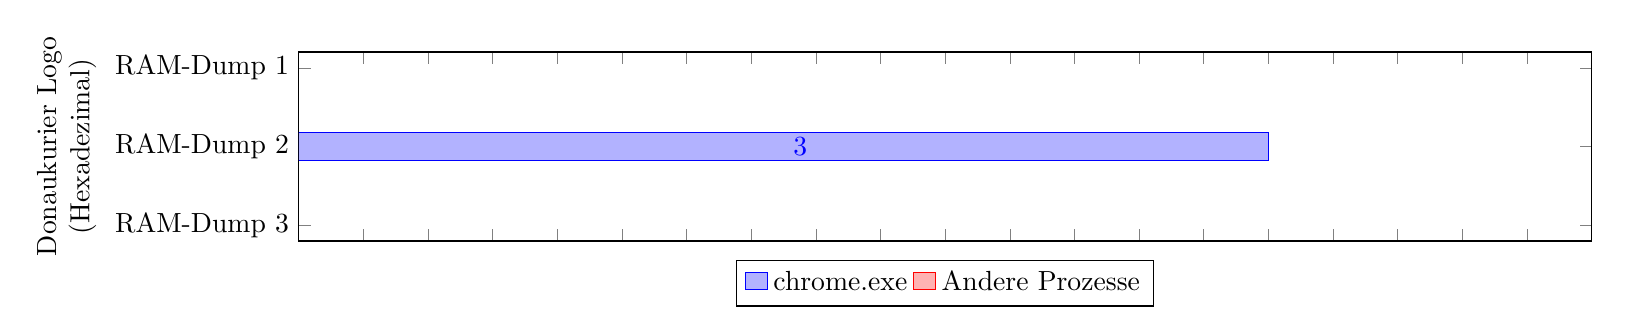
\begin{tikzpicture}
				\begin{axis}[
					xbar stacked,
					width=18cm, 
					height=12cm, 
					ylabel style={align=center}, ylabel=Donaukurier Logo\\(Hexadezimal),
					y=1cm,
					symbolic y coords={RAM-Dump 3, RAM-Dump 2, RAM-Dump 1},
					ytick=data,
					xticklabels={,,},
					xmin = 0,
					xmax = 4,
					nodes near coords, 
					nodes near coords align={horizontal},
					legend style={
						at={(0.5,-0.1)},
						anchor=north
					},
					legend columns=2
					]
					\addplot coordinates {
						(0,RAM-Dump 3) (3,RAM-Dump 2) (0,RAM-Dump 1)
					};
					\addplot coordinates {
						(0,RAM-Dump 3) (0,RAM-Dump 2) (0,RAM-Dump 1)
					};
					\legend{chrome.exe, Andere Prozesse}
				\end{axis}
			\end{tikzpicture}
		\end{tabular}
	}
	\caption{Anzahl gefundener Hexadezimalwerte des Donaukurier-Logos im Chrome RAM}
	\label{chart:chrome-volatility-image}
\end{table}

\subsection*{Registry}\label{chap:ergebnisse-chrome-uncommon-registry}

Wie in [link Kapitel] bereits beschrieben, zählt die Analyse der Registry sowohl zu den Common als auch zu den Uncommon Locations. Es können weder in den \glqq{}SetValue\grqq{}-Operationen in den Process Monitor Logs noch durch die Analyse der System- und User-Hives durch den RegistryExplorer Artefakte gefunden werden. Eine weitergehende Analyse der Registry ist im \autoref{chap:anhang-chrome-common-registry} und \autoref{chap:anhang-chrome-uncommon-registry} beschrieben.
% Aufführen aller Registry-Schreiboperationen, wie analysiert, 

\section{Brave}\label{chap:ergebnisse-brave}

\begin{comment}

Analyse aller Schreiboperationen mittels des ProcessMonitors:

2 Logs aufgezeichnet gemäß [link], Analyse in getrennten Kapiteln

\subsubsection*{Process Monitor Log 1}

Unterschieden in bekannte Browser-Pfade (Browser-Pfad) und andere Pfade (außerhalb des typischen Browser-Pfades)

Bekannt:

Glob gegliedert in Dateiendungen, mit möglichen Erklärungen: \\
\begin{comment}
- 000003.log's:  \\
- tmp \\
- png \\
- store\_new \\
- .Identifier \\
- .db  \\
- LOG \\
- .pb \\
- .ftlite \\
- .dbtemp \\
- others -> Erklärung der Datenbanken + locations

=> Zusammenfassung in Tabelle \\\\

Unbekannter Pfad:\\
- tmp files, nicht mehr auffindbar\\
- 


Alle Schreiboperationen mit aufnehmen in Anhang evtl.

\subsubsection*{Process Monitor Log 2}

Hier Erklärungen zu 2. mit Tabelle rein

\subsubsection*{Databases}

Welche Datenbanken sind wann vorhanden? Was verändert sich über die Zeit? Textuell + Tabellarisch zeigen!

\subsection*{Registry}

\subsubsection*{Process Monitor}

Zuerst die im Process Monitor aufgeze

\subsubsection*{Hives-Extraction inklusive Analyse}

Dann Auslesen der bereits in [link] dargestellten Hives + Einlesen in Registry Explorer. Liefert bei allen 3 betrachteten Snapshots keine Ergebnisse

\subsection*{Black-Box Analyse/Uncommon Locations}

\subsubsection*{Analyse mit Autopsy}

\subsubsection*{Analyse mit Volatility}

Jeweils schöne Tabellen hierzu:

Keywords\\
URL\\
Mail \\
HTTP inkl. Screenshots hier (Verweis nach oben)

Image + Summary Tabellen hier am Ende no!

\end{comment}

Abschließend werden in diesem Kapitel die Analyseergebnisse des Browsers Brave dargelegt, wobei diese wieder, wie in den vorherigen Kapiteln, in Common Locations, Uncommon Locations und der Registry unterschieden werden.

\subsection*{Common Locations}\label{chap:ergebnisse-brave-common-locations}

Zu Beginn erfolgt die Untersuchung der Common Locations auf potenzielle private Browsing Artefakte. Bei der Analyse der Schreiboperationen aus den Process Monitor Logfiles konnten keine Artefakte befunden werden, wie es auch bei der Untersuchung der SQLite-Datenbanken der Fall war.\\
Eine umfangreiche Auswertung der Daten sowie den Datenbänken befindet sich im \autoref{chap:anhang-brave-common-locations}.

\subsection*{Uncommon Locations}\label{chap:ergebnisse-brave-uncommon-locations}

Anschließend an die Common Locations folgt nun die Untersuchung der Uncommon Locations. Dafür werden vollständige Speicherabbilder nach Artefakten der privaten Browsing-Session untersucht. Für diesen Zweck werden die beiden Forensik-Programme Autopsy und Volatility verwendet.

\subsubsection*{Analyse mit Autopsy}\label{chap:ergebnisse-brave-uncommon-locations-autopsy}

Autopsy wird bei den Uncommon Locations zusätzlich als forensisches Werkzeug verwendet im Gegensatz zur Analyse der Common Locations, bei welchen es eingesetzt wurde, um Dateien aus den Snapshots zu extrahieren.\\
Zunächst wurde die Stringsuche gemäß [link Kapitel] eingesetzt, wobei es keine Suchtreffer gab.\\
Zusätzlich wurden automatisch kategorisierte Dateien untersucht, wobei hier auch keine Artefakte zu finden waren. \autoref{chap:anhang-brave-uncommon-locations-autopsy} geht auf diese Dateien ausführlicher ein.

\subsubsection*{Analyse mit Volatility}\label{chap:ergebnisse-brave-uncommon-locations-volatility}

Für die Analyse des Arbeitsspeichers wurde das Forensik-Tool Volatility verwendet, womit eine Stringsuche mittels des Plugins Yarascan durchgeführt wird. Damit durchsucht man ein Arbeitsspeicherabbild nach gewissen Strings, welche zuvor in einer yara-rule festgelegt werden können. Die für diese Arbeit verwendete Datei inklusive der Regeln ist in [link Anhang runter] aufgeführt. 

\paragraph*{Yara-Regel \glqq{}HTML\grqq{}}\label{chap:ergebnisse-brave-uncommon-locations-volatility-html}

Beim Brave-Browser konnte ein HTML-Fragment wiederhergestellt werden, was in \autoref{chart:brave-volatility-htmls} dargestellt ist. Es ist wieder der String \glqq{}>Themen:\grqq, welcher einmal im zweiten RAM-Dump vorliegt.

\begin{table}[h!]
	\resizebox{\linewidth}{!}{
		\begin{tabular}{l}	
			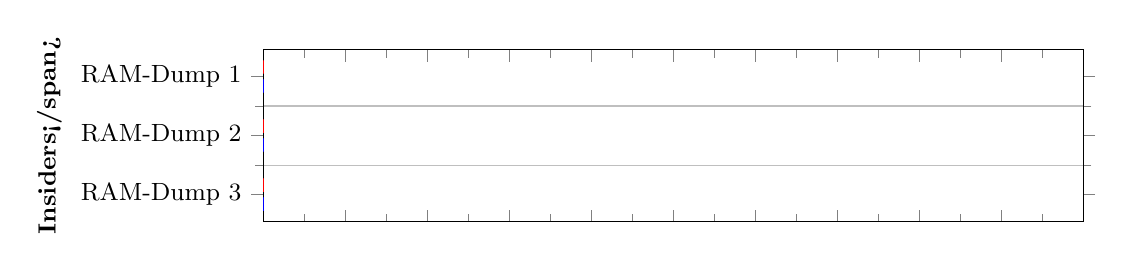
\begin{tikzpicture}
				\begin{axis}[
					xbar,
					width=12cm, 
					height=3cm, 
					ylabel style={align=center}, ylabel=\textbf{Insiders</span>},
					y=0.75cm,
					symbolic y coords={RAM-Dump 3, RAM-Dump 2, RAM-Dump 1},
					label style={font=\small},
					tick label style={font=\small},
					ytick=data,
					xticklabels={,,},
					xmin = 0,
					xmax = 5,
					nodes near coords, 
					nodes near coords align={horizontal},
					nodes near coords style={font=\tiny},
					nodes near coords={\pgfmathfloatifflags{\pgfplotspointmeta}{0}{}{\pgfmathprintnumber{\pgfplotspointmeta}}},
					bar width=.17cm,
					enlarge y limits={abs=2*\pgfplotbarwidth},
					scaled x ticks=false,
					legend style={
						at={(0.5,-0.1)},
						anchor=north
					},
					legend columns=3,
					yminorgrids = true,minor tick num=1
					]
					\addplot coordinates {
						(0,RAM-Dump 3) (0,RAM-Dump 2) (0,RAM-Dump 1)
					};
					\addplot coordinates {
						(0,RAM-Dump 3) (0,RAM-Dump 2) (0,RAM-Dump 1)
					};
				\end{axis}
			\end{tikzpicture}
			\\[-7pt]
			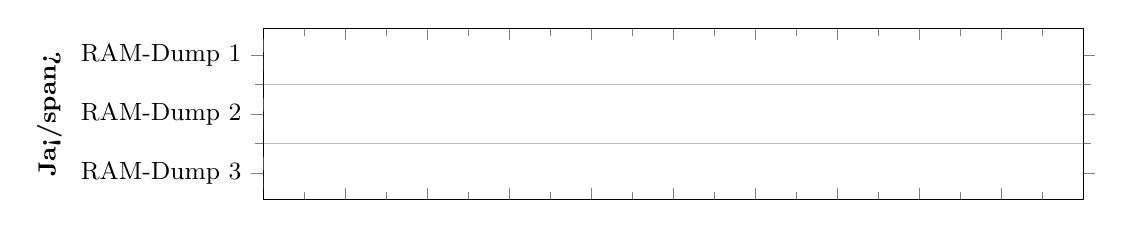
\begin{tikzpicture}
				\begin{axis}[
					xbar,
					width=12cm, 
					height=3cm, 
					ylabel style={align=center}, ylabel=\textbf{Ja</span>},
					y=0.75cm,
					symbolic y coords={RAM-Dump 3, RAM-Dump 2, RAM-Dump 1},
					label style={font=\small},
					tick label style={font=\small},
					ytick=data,
					xticklabels={,,},
					xmin = 0,
					xmax = 5,
					nodes near coords, 
					nodes near coords align={horizontal},
					nodes near coords style={font=\tiny},
					nodes near coords={\pgfmathfloatifflags{\pgfplotspointmeta}{0}{}{\pgfmathprintnumber{\pgfplotspointmeta}}},
					bar width=.17cm,
					enlarge y limits={abs=2*\pgfplotbarwidth},
					scaled x ticks=false,
					legend style={
						at={(0.5,-0.1)},
						anchor=north
					},
					legend columns=3,
					yminorgrids = true,minor tick num=1
					]
					\addplot coordinates {
						(0,RAM-Dump 3)  (0,RAM-Dump 2) (0,RAM-Dump 1)
					};
					\addplot coordinates {
						(0,RAM-Dump 3)  (0,RAM-Dump 2) (0,RAM-Dump 1)
					};
				\end{axis}
			\end{tikzpicture}
			\\[-7pt]
			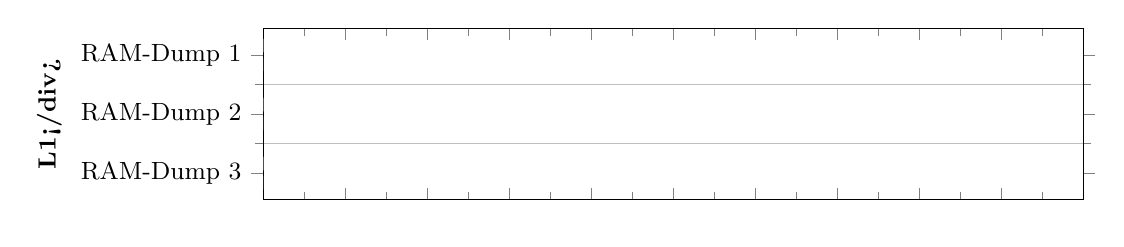
\begin{tikzpicture}
				\begin{axis}[
					xbar,
					width=12cm, 
					height=3cm, 
					ylabel style={align=center}, ylabel=\textbf{L1</div>},
					y=0.75cm,
					symbolic y coords={RAM-Dump 3, RAM-Dump 2, RAM-Dump 1},
					label style={font=\small},
					tick label style={font=\small},
					ytick=data,
					xticklabels={,,},
					xmin = 0,
					xmax = 5,
					nodes near coords, 
					nodes near coords align={horizontal},
					nodes near coords style={font=\tiny},
					nodes near coords={\pgfmathfloatifflags{\pgfplotspointmeta}{0}{}{\pgfmathprintnumber{\pgfplotspointmeta}}},
					bar width=.17cm,
					enlarge y limits={abs=2*\pgfplotbarwidth},
					scaled x ticks=false,
					legend style={
						at={(0.5,-0.1)},
						anchor=north
					},
					legend columns=3,
					yminorgrids = true,minor tick num=1
					]
					\addplot coordinates {
						(0,RAM-Dump 3)  (0,RAM-Dump 2) (0,RAM-Dump 1)
					};
					\addplot coordinates {
						(0,RAM-Dump 3)  (0,RAM-Dump 2) (0,RAM-Dump 1)
					};
				\end{axis}
			\end{tikzpicture}
			\\[-7pt]
			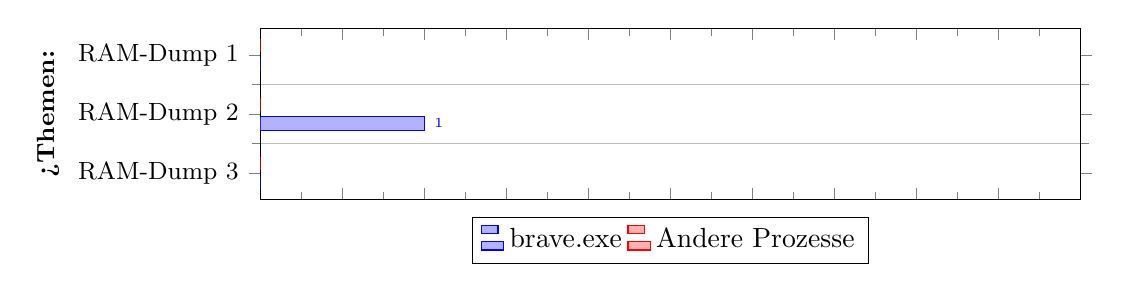
\begin{tikzpicture}
				\begin{axis}[
					xbar,
					width=12cm, 
					height=3cm, 
					ylabel style={align=center}, ylabel=\textbf{>Themen:},
					y=0.75cm,
					symbolic y coords={RAM-Dump 3, RAM-Dump 2, RAM-Dump 1},
					label style={font=\small},
					tick label style={font=\small},
					ytick=data,
					xticklabels={,,},
					xmin = 0,
					xmax = 5,
					nodes near coords, 
					nodes near coords align={horizontal},
					nodes near coords style={font=\tiny},
					nodes near coords={\pgfmathfloatifflags{\pgfplotspointmeta}{0}{}{\pgfmathprintnumber{\pgfplotspointmeta}}},
					bar width=.17cm,
					enlarge y limits={abs=2*\pgfplotbarwidth},
					scaled x ticks=false,
					legend style={
						at={(0.5,-0.1)},
						anchor=north
					},
					legend columns=3,
					yminorgrids = true,minor tick num=1
					]
					\addplot coordinates {
						(0,RAM-Dump 3)  (1,RAM-Dump 2) (0,RAM-Dump 1)
					};
					\addplot coordinates {
						(0,RAM-Dump 3)  (0,RAM-Dump 2) (0,RAM-Dump 1)
					};
					\legend{brave.exe, Andere Prozesse}
				\end{axis}
			\end{tikzpicture}
		\end{tabular}
	}
	\caption{Anzahl gefundener HTML-Fragmente im Brave RAM}
	\label{chart:brave-volatility-htmls}
\end{table}

Die Extraktion der kompletten Webseite war dabei wie in [link nach oben] möglich. Auch das Vorgehen war identisch, außer, wie zu erwarten war, die virtuellen und physikalischen Adressen der verschiedenen Strings. Daher wird hier nicht nochmal ausführlich auf das Vorgehen der Extraktion der Webseite aufgeführt.\\
Anschließend an die Wiederherstellung der HTML-Datei wurden die beiden extrahierten Dateien nochmals gegeneinander verglichen. \autoref{pic:compareHTMLs} zeigt dies anhand der compre-Funktionalität von Visual Studio Code. An der rechten Seite in der Bildlaufleiste sind die Sektionen farbig dargestellt, welche Unterschiede aufweisen. Dabei wurde durch Analyse derer deutlich, dass der Aufbau und die Struktur beider extrahierter Webseiten übereinstimmt, es nur geringe Unterschiede bei einigen Namen der Artikel und Meldungen gibt. Auch sind die Dateien auch (nahezu) identisch groß (290kB).
%\autoref{pic:brave-vimdiff} zeigt einen Ausschnitt eines generierten HTML-Reports, welcher mittels \textit{vimdiff} in der Version 9.0 erstellt wurde und die beiden HTML-Seiten vergleicht. Der genaue Befehl lautete dabei: \\ \texttt{vimdiff -c TOhtml -c "w vimdiff\_export.html | qa!" donaukurier\_recovered.html donaukurier\_recovered\_brave.html}

\begin{figure}[h!]
	\centering
	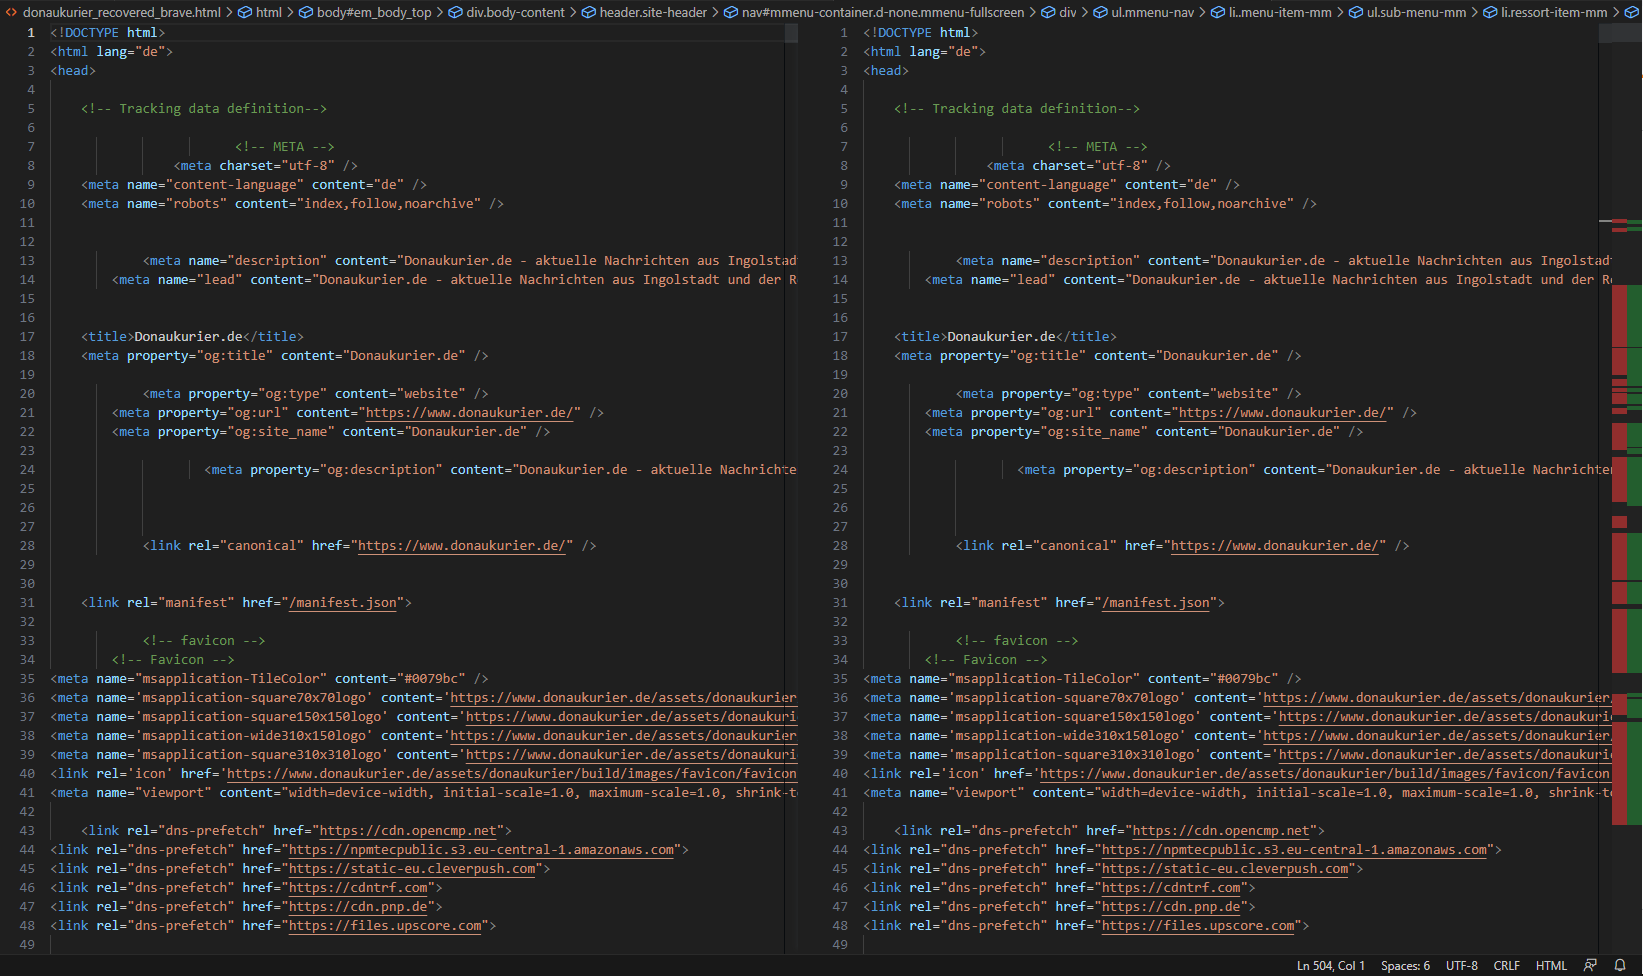
\includegraphics[width=\textwidth]{Donaukurier1.png}
	\caption{Ausschnitt aus VS Code mit dem Vergleich der beiden Donaukurier Webseiten}
	\label{pic:compareHTMLs}
\end{figure}

\paragraph*{Yara-Regel \glqq{}Suchbegriffe\grqq{}}\label{chap:ergebnisse-brave-uncommon-locations-volatility-suchbegriffe}  

\autoref{chart:brave-volatility-keywords} zeigt, dass alle der vier Suchbegriffe jeweils gefunden wurden, jedoch nur im zweiten RAM-Dump, also nach der Durchführung des Browsing-Szenarios bei noch geöffnetem Browser. Der String \glqq{}pfaffenhofen\grqq{} wurde dabei am häufigsten mit 1447 Treffern, \glqq{}nanoradar\grqq{} am seltensten mit nur 51 Suchergebnissen gefunden. Dabei wurden auch alle Suchbegriffe rein in Brave-Prozessen ausfindig gemacht.

\begin{table}[h!]
	\resizebox{\linewidth}{!}{
		\begin{tabular}{l}	
			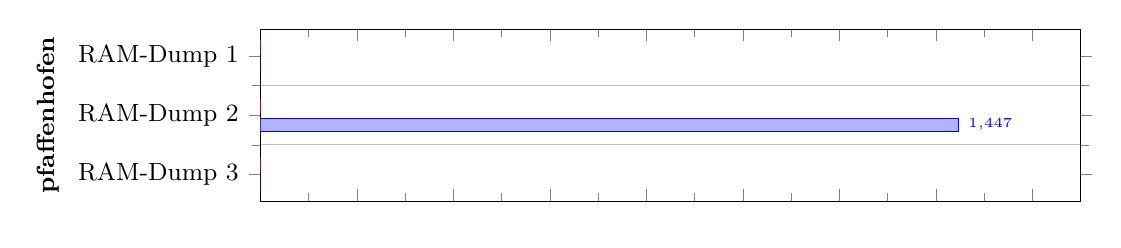
\begin{tikzpicture}
				\begin{axis}[
					xbar,
					width=12cm, 
					height=3cm, 
					ylabel style={align=center}, ylabel=\textbf{pfaffenhofen},
					y=0.75cm,
					symbolic y coords={RAM-Dump 3, RAM-Dump 2, RAM-Dump 1},
					label style={font=\small},
					tick label style={font=\small},
					ytick=data,
					xticklabels={,,},
					xmin = 0,
					xmax = 1700,
					nodes near coords, 
					nodes near coords align={horizontal},
					nodes near coords style={font=\tiny},
					nodes near coords={\pgfmathfloatifflags{\pgfplotspointmeta}{0}{}{\pgfmathprintnumber{\pgfplotspointmeta}}},
					bar width=.17cm,
					enlarge y limits={abs=2*\pgfplotbarwidth},
					scaled x ticks=false,
					legend style={
						at={(0.5,-0.1)},
						anchor=north
					},
					legend columns=3,
					yminorgrids = true,minor tick num=1
					]
					\addplot coordinates {
						(0,RAM-Dump 3) (1447,RAM-Dump 2) (0,RAM-Dump 1)
					};
					\addplot coordinates {
						(0,RAM-Dump 3) (0,RAM-Dump 2) (0,RAM-Dump 1)
					};
				\end{axis}
			\end{tikzpicture}
			\\[-7pt]
			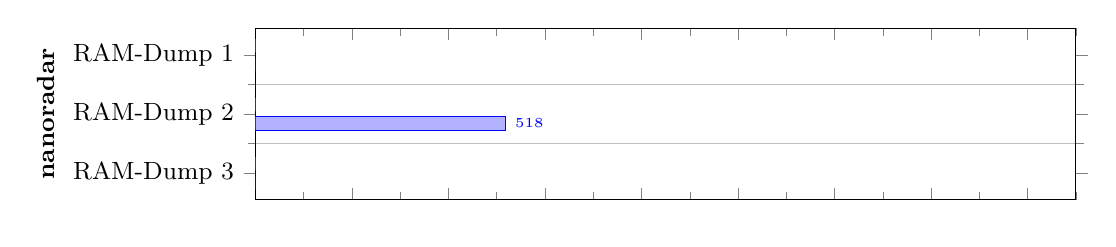
\begin{tikzpicture}
				\begin{axis}[
					xbar,
					width=12cm, 
					height=3cm, 
					ylabel style={align=center}, ylabel=\textbf{nanoradar},
					y=0.75cm,
					symbolic y coords={RAM-Dump 3, RAM-Dump 2, RAM-Dump 1},
					label style={font=\small},
					tick label style={font=\small},
					ytick=data,
					xticklabels={,,},
					xmin = 0,
					xmax = 1700,
					nodes near coords, 
					nodes near coords align={horizontal},
					nodes near coords style={font=\tiny},
					nodes near coords={\pgfmathfloatifflags{\pgfplotspointmeta}{0}{}{\pgfmathprintnumber{\pgfplotspointmeta}}},
					bar width=.17cm,
					enlarge y limits={abs=2*\pgfplotbarwidth},
					scaled x ticks=false,
					legend style={
						at={(0.5,-0.1)},
						anchor=north
					},
					legend columns=3,
					yminorgrids = true,minor tick num=1
					]
					\addplot coordinates {
						(0,RAM-Dump 3)  (518,RAM-Dump 2) (0,RAM-Dump 1)
					};
					\addplot coordinates {
						(0,RAM-Dump 3)  (0,RAM-Dump 2) (0,RAM-Dump 1)
					};
				\end{axis}
			\end{tikzpicture}
			\\[-7pt]
			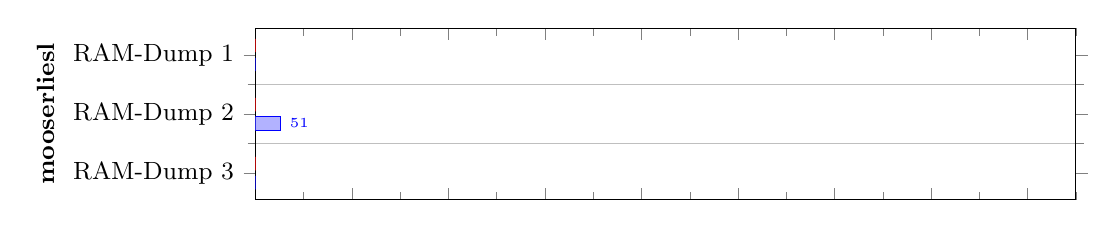
\begin{tikzpicture}
				\begin{axis}[
					xbar,
					width=12cm, 
					height=3cm, 
					ylabel style={align=center}, ylabel=\textbf{mooserliesl},
					y=0.75cm,
					symbolic y coords={RAM-Dump 3, RAM-Dump 2, RAM-Dump 1},
					label style={font=\small},
					tick label style={font=\small},
					ytick=data,
					xticklabels={,,},
					xmin = 0,
					xmax = 1700,
					nodes near coords, 
					nodes near coords align={horizontal},
					nodes near coords style={font=\tiny},
					nodes near coords={\pgfmathfloatifflags{\pgfplotspointmeta}{0}{}{\pgfmathprintnumber{\pgfplotspointmeta}}},
					bar width=.17cm,
					enlarge y limits={abs=2*\pgfplotbarwidth},
					scaled x ticks=false,
					legend style={
						at={(0.5,-0.1)},
						anchor=north
					},
					legend columns=3,
					yminorgrids = true,minor tick num=1
					]
					\addplot coordinates {
						(0,RAM-Dump 3)  (51,RAM-Dump 2) (0,RAM-Dump 1)
					};
					\addplot coordinates {
						(0,RAM-Dump 3)  (0,RAM-Dump 2) (0,RAM-Dump 1)
					};
				\end{axis}
			\end{tikzpicture}
			\\[-7pt]
			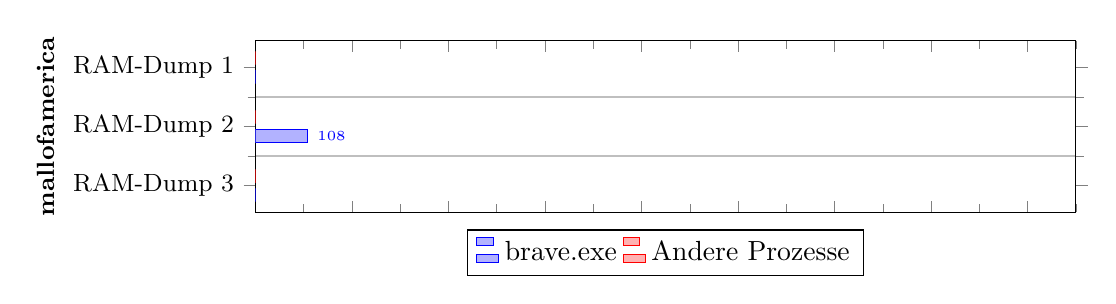
\begin{tikzpicture}
				\begin{axis}[
					xbar,
					width=12cm, 
					height=3cm, 
					ylabel style={align=center}, ylabel=\textbf{mallofamerica},
					y=0.75cm,
					symbolic y coords={RAM-Dump 3, RAM-Dump 2, RAM-Dump 1},
					label style={font=\small},
					tick label style={font=\small},
					ytick=data,
					xticklabels={,,},
					xmin = 0,
					xmax = 1700,
					nodes near coords, 
					nodes near coords align={horizontal},
					nodes near coords style={font=\tiny},
					nodes near coords={\pgfmathfloatifflags{\pgfplotspointmeta}{0}{}{\pgfmathprintnumber{\pgfplotspointmeta}}},
					bar width=.17cm,
					enlarge y limits={abs=2*\pgfplotbarwidth},
					scaled x ticks=false,
					legend style={
						at={(0.5,-0.1)},
						anchor=north
					},
					legend columns=3,
					yminorgrids = true,minor tick num=1
					]
					\addplot coordinates {
						(0,RAM-Dump 3)  (108,RAM-Dump 2) (0,RAM-Dump 1)
					};
					\addplot coordinates {
						(0,RAM-Dump 3)  (0,RAM-Dump 2) (0,RAM-Dump 1)
					};
					\legend{brave.exe, Andere Prozesse}
				\end{axis}
			\end{tikzpicture}
		\end{tabular}
	}
	\caption{Anzahl gefundener Suchbegriffe im Brave RAM}
	\label{chart:brave-volatility-keywords}
\end{table}
%TODO Vergleich Google Duckduckgo

\paragraph*{Yara-Regel \glqq{}URLs\grqq{}}\label{chap:ergebnisse-brave-uncommon-locations-volatility-urls}

Auch bei der URL-Yara-Rule konnte wieder alle URLs im RAM nachgewiesen werden. Bei \glqq{}donaukurier.de\grqq{} gab es sogar einen Treffer im dritten RAM-Dump, alle anderen waren nur im zweiten Speicherabbild auffindbar. Dabei waren es auch bei der Donaukurier-URL die meisten Treffer mit insgesamt 3514 Artefakten, wobei sechs davon in anderen Prozessen neben Brave gefunden wurden. Sehr präsent war hier der Prozess \glqq{}NisSrv.exe\grqq{}. Dieser ist ein Teil des Microsoft Defenders \cite{pogonin2022microsoft}, was grundsätzlich merkwürdig erscheint, sich aber dadurch erklären lässt, dass dieser vielleicht im Hintergrund den Datenverkehr mitliest und entscheidet, ob gewisse Aktivitäten in Ordnung sind oder evtl. ein Virus oder anderweitige bösartige Software unsicheren Netzwerkverkehr tätigt.

\begin{table}[h!]
	\resizebox{\linewidth}{!}{
		\begin{tabular}{l}	
			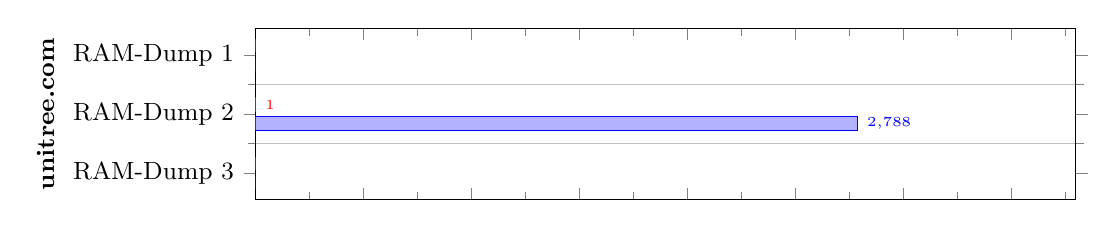
\begin{tikzpicture}
				\begin{axis}[
					xbar,
					width=12cm, 
					height=3cm, 
					ylabel style={align=center}, ylabel=\textbf{unitree.com},
					y=0.75cm,
					symbolic y coords={RAM-Dump 3, RAM-Dump 2, RAM-Dump 1},
					label style={font=\small},
					tick label style={font=\small},
					ytick=data,
					xticklabels={,,},
					xmin = 0,
					xmax = 3800,
					nodes near coords, 
					nodes near coords align={horizontal},
					nodes near coords style={font=\tiny},
					nodes near coords={\pgfmathfloatifflags{\pgfplotspointmeta}{0}{}{\pgfmathprintnumber{\pgfplotspointmeta}}},
					bar width=.17cm,
					enlarge y limits={abs=2*\pgfplotbarwidth},
					scaled x ticks=false,
					legend style={
						at={(0.5,-0.1)},
						anchor=north
					},
					legend columns=3,
					yminorgrids = true,minor tick num=1
					]
					\addplot coordinates {
						(0,RAM-Dump 3) (2788,RAM-Dump 2) (0,RAM-Dump 1)
					};
					\addplot coordinates {
						(0,RAM-Dump 3) (1,RAM-Dump 2) (0,RAM-Dump 1)
					};
				\end{axis}
			\end{tikzpicture}
			\\[-7pt]
			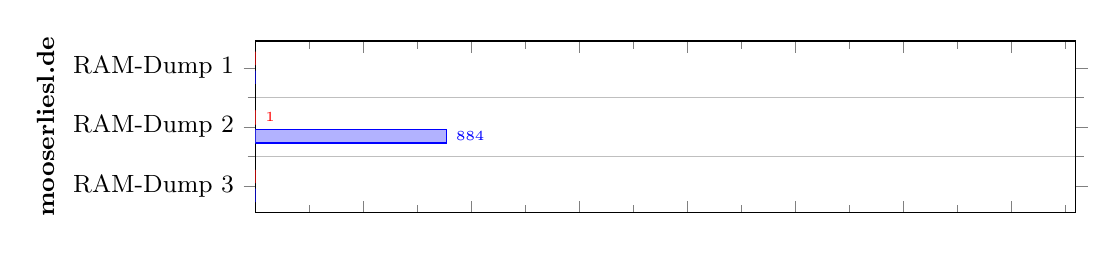
\begin{tikzpicture}
				\begin{axis}[
					xbar,
					width=12cm, 
					height=3cm, 
					ylabel style={align=center}, ylabel=\textbf{mooserliesl.de},
					y=0.75cm,
					symbolic y coords={RAM-Dump 3, RAM-Dump 2, RAM-Dump 1},
					label style={font=\small},
					tick label style={font=\small},
					ytick=data,
					xticklabels={,,},
					xmin = 0,
					xmax = 3800,
					nodes near coords, 
					nodes near coords align={horizontal},
					nodes near coords style={font=\tiny},
					nodes near coords={\pgfmathfloatifflags{\pgfplotspointmeta}{0}{}{\pgfmathprintnumber{\pgfplotspointmeta}}},
					bar width=.17cm,
					enlarge y limits={abs=2*\pgfplotbarwidth},
					scaled x ticks=false,
					legend style={
						at={(0.5,-0.1)},
						anchor=north
					},
					legend columns=3,
					yminorgrids = true,minor tick num=1
					]
					\addplot coordinates {
						(0,RAM-Dump 3) (884,RAM-Dump 2) (0,RAM-Dump 1)
					};
					\addplot coordinates {
						(0,RAM-Dump 3) (1,RAM-Dump 2) (0,RAM-Dump 1)
					};
				\end{axis}
			\end{tikzpicture}	
			\\[-7pt]
			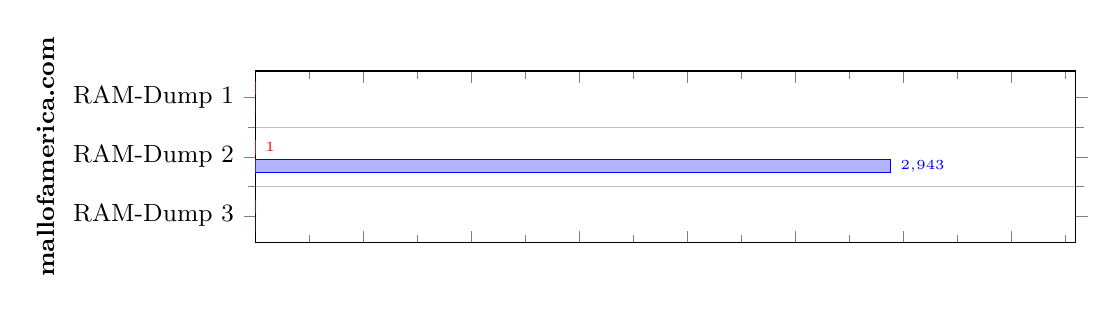
\begin{tikzpicture}
				\begin{axis}[
					xbar,
					width=12cm, 
					height=3cm, 
					ylabel style={align=center}, ylabel=\textbf{mallofamerica.com},
					y=0.75cm,
					symbolic y coords={RAM-Dump 3, RAM-Dump 2, RAM-Dump 1},
					label style={font=\small},
					tick label style={font=\small},
					ytick=data,
					xticklabels={,,},
					xmin = 0,
					xmax = 3800,
					nodes near coords, 
					nodes near coords align={horizontal},
					nodes near coords style={font=\tiny},
					nodes near coords={\pgfmathfloatifflags{\pgfplotspointmeta}{0}{}{\pgfmathprintnumber{\pgfplotspointmeta}}},
					bar width=.17cm,
					enlarge y limits={abs=2*\pgfplotbarwidth},
					scaled x ticks=false,
					legend style={
						at={(0.5,-0.1)},
						anchor=north
					},
					legend columns=3,
					yminorgrids = true,minor tick num=1
					]
					\addplot coordinates {
						(0,RAM-Dump 3) (2943,RAM-Dump 2) (0,RAM-Dump 1)
					};
					\addplot coordinates {
						(0,RAM-Dump 3) (1,RAM-Dump 2) (0,RAM-Dump 1)
					};
				\end{axis}
			\end{tikzpicture}
			\\[-7pt]
			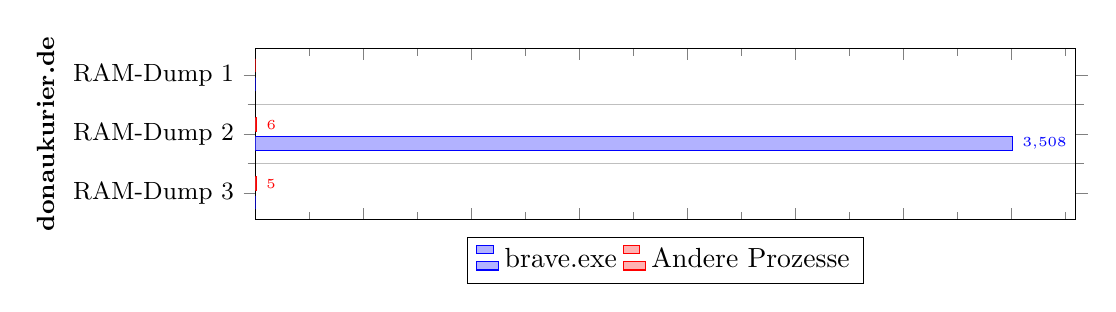
\begin{tikzpicture}
				\begin{axis}[
					xbar,
					width=12cm, 
					height=3cm, 
					ylabel style={align=center}, ylabel=\textbf{donaukurier.de},
					y=0.75cm,
					symbolic y coords={RAM-Dump 3, RAM-Dump 2, RAM-Dump 1},
					label style={font=\small},
					tick label style={font=\small},
					ytick=data,
					xticklabels={,,},
					xmin = 0,
					xmax = 3800,
					nodes near coords, 
					nodes near coords align={horizontal},
					nodes near coords style={font=\tiny},
					nodes near coords={\pgfmathfloatifflags{\pgfplotspointmeta}{0}{}{\pgfmathprintnumber{\pgfplotspointmeta}}},
					bar width=.17cm,
					enlarge y limits={abs=2*\pgfplotbarwidth},
					scaled x ticks=false,
					legend style={
						at={(0.5,-0.1)},
						anchor=north
					},
					legend columns=3,
					yminorgrids = true,minor tick num=1
					]
					\addplot coordinates {
						(0,RAM-Dump 3) (3508,RAM-Dump 2) (0,RAM-Dump 1)
					};
					\addplot coordinates {
						(5,RAM-Dump 3) (6,RAM-Dump 2) (0,RAM-Dump 1)
					};
					\legend{brave.exe, Andere Prozesse}
				\end{axis}
			\end{tikzpicture}		
		\end{tabular}
	}
	\caption{Anzahl gefundener URLs im Brave RAM}
	\label{chart:brave-volatility-urls}
\end{table}

\paragraph*{Yara-Regel \glqq{}E-Mail\grqq{}}\label{chap:ergebnisse-brave-uncommon-locations-volatility-email}

Wie in \autoref{chart:brave-volatility-mail} dargestellt, wurden im zweiten als auch im dritten Arbeitsspeicherabbild Artefakte bzgl. der Yara-Regel \glqq{}E-Mail\grqq{} gefunden. Davon waren die meisten bei der E-Mail-Adresse \glqq{}computerforensikvl@gmail.com\grqq{} mit insgesamt 134 Suchtreffern vorhanden. 9 dieser waren aus anderen Prozessen, die restlichen 125 waren direkt in einem Speicherbereich des Chrome-Browsers zu finden. Bei dieser wurde auch noch ein Artefakt im dritten RAM-Dump gefunden im Speicherbereich des dwm.exe Prozesses, welcher zuvor bereits angesprochen wurde. Am wenigsten Suchtreffer hab es bei dem Betrefftext.

\begin{table}[h!]
	\resizebox{\linewidth}{!}{
		\begin{tabular}{r}	
			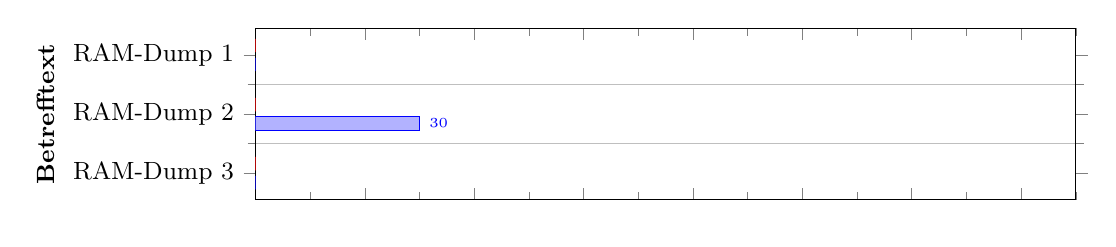
\begin{tikzpicture}
				\begin{axis}[
					xbar,
					width=12cm, 
					height=3cm, 
					ylabel style={align=center}, ylabel=\textbf{Betrefftext},
					y=0.75cm,
					symbolic y coords={RAM-Dump 3, RAM-Dump 2, RAM-Dump 1},
					label style={font=\small},
					tick label style={font=\small},
					ytick=data,
					xticklabels={,,},
					xmin = 0,
					xmax = 150,
					nodes near coords, 
					nodes near coords align={horizontal},
					nodes near coords style={font=\tiny},
					nodes near coords={\pgfmathfloatifflags{\pgfplotspointmeta}{0}{}{\pgfmathprintnumber{\pgfplotspointmeta}}},
					bar width=.17cm,
					enlarge y limits={abs=2*\pgfplotbarwidth},
					scaled x ticks=false,
					legend style={
						at={(0.5,-0.1)},
						anchor=north
					},
					legend columns=3,
					yminorgrids = true,minor tick num=1
					]
					\addplot coordinates {
						(0,RAM-Dump 3) (30,RAM-Dump 2) (0,RAM-Dump 1)
					};
					\addplot coordinates {
						(0,RAM-Dump 3) (0,RAM-Dump 2) (0,RAM-Dump 1)
					};
					%				\legend{firefox.exe, Andere Prozesse}
				\end{axis}
			\end{tikzpicture}
			\\[-7pt]
			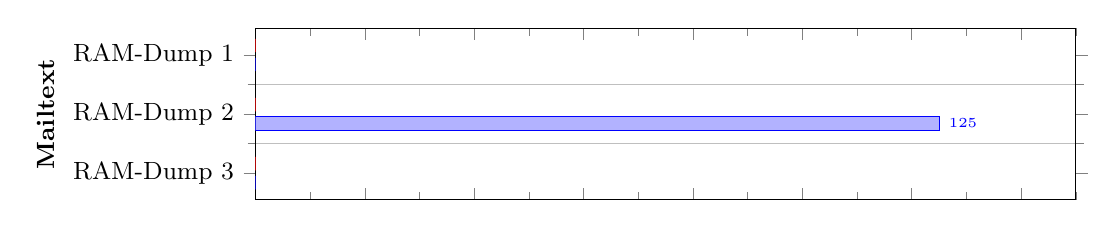
\begin{tikzpicture}
				\begin{axis}[
					xbar,
					width=12cm, 
					height=3cm, 
					ylabel style={align=center}, ylabel=\textbf{Mailtext},
					y=0.75cm,
					symbolic y coords={RAM-Dump 3, RAM-Dump 2, RAM-Dump 1},
					label style={font=\small},
					tick label style={font=\small},
					ytick=data,
					xticklabels={,,},
					xmin = 0,
					xmax = 150,
					nodes near coords, 
					nodes near coords align={horizontal},
					nodes near coords style={font=\tiny},
					nodes near coords={\pgfmathfloatifflags{\pgfplotspointmeta}{0}{}{\pgfmathprintnumber{\pgfplotspointmeta}}},
					bar width=.17cm,
					enlarge y limits={abs=2*\pgfplotbarwidth},
					scaled x ticks=false,
					legend style={
						at={(0.5,-0.1)},
						anchor=north
					},
					legend columns=3,
					yminorgrids = true,minor tick num=1
					]
					\addplot coordinates {
						(0,RAM-Dump 3) (125,RAM-Dump 2) (0,RAM-Dump 1)
					};
					\addplot coordinates {
						(0,RAM-Dump 3) (0,RAM-Dump 2) (0,RAM-Dump 1)
					};
					%				\legend{firefox.exe, Andere Prozesse}
				\end{axis}
			\end{tikzpicture}	
			\\[-7pt]
			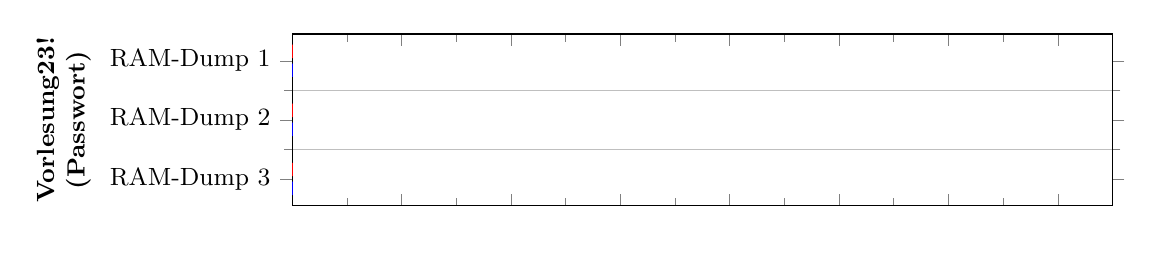
\begin{tikzpicture}
				\begin{axis}[
					xbar,
					width=12cm, 
					height=3cm, 
					ylabel style={align=center}, ylabel=\textbf{Vorlesung23!}\\\textbf{(Passwort)},
					y=0.75cm,
					symbolic y coords={RAM-Dump 3, RAM-Dump 2, RAM-Dump 1},
					label style={font=\small},
					tick label style={font=\small},
					ytick=data,
					xticklabels={,,},
					xmin = 0,
					xmax = 150,
					nodes near coords, 
					nodes near coords align={horizontal},
					nodes near coords style={font=\tiny},
					nodes near coords={\pgfmathfloatifflags{\pgfplotspointmeta}{0}{}{\pgfmathprintnumber{\pgfplotspointmeta}}},
					bar width=.17cm,
					enlarge y limits={abs=2*\pgfplotbarwidth},
					scaled x ticks=false,
					legend style={
						at={(0.5,-0.1)},
						anchor=north
					},
					legend columns=3,
					yminorgrids = true,minor tick num=1
					]
					\addplot coordinates {
						(0,RAM-Dump 3) (0,RAM-Dump 2) (0,RAM-Dump 1)
					};
					\addplot coordinates {
						(0,RAM-Dump 3) (0,RAM-Dump 2) (0,RAM-Dump 1)
					};
					%				\legend{firefox.exe, Andere Prozesse}
				\end{axis}
			\end{tikzpicture}
			\\[-7pt]
			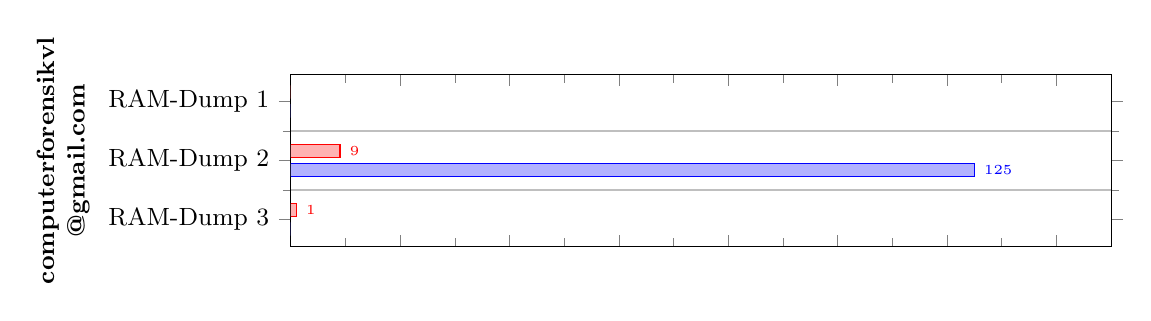
\begin{tikzpicture}
				\begin{axis}[
					xbar,
					width=12cm, 
					height=3cm, 
					ylabel style={align=center}, ylabel=\textbf{computerforensikvl}\\\textbf{@gmail.com},
					y=0.75cm,
					symbolic y coords={RAM-Dump 3, RAM-Dump 2, RAM-Dump 1},
					label style={font=\small},
					tick label style={font=\small},
					ytick=data,
					xticklabels={,,},
					xmin = 0,
					xmax = 150,
					nodes near coords, 
					nodes near coords align={horizontal},
					nodes near coords style={font=\tiny},
					nodes near coords={\pgfmathfloatifflags{\pgfplotspointmeta}{0}{}{\pgfmathprintnumber{\pgfplotspointmeta}}},
					bar width=.17cm,
					enlarge y limits={abs=2*\pgfplotbarwidth},
					scaled x ticks=false,
					legend style={
						at={(0.5,-0.1)},
						anchor=north
					},
					legend columns=3,
					yminorgrids = true,minor tick num=1
					]
					\addplot coordinates {
						(0,RAM-Dump 3) (125,RAM-Dump 2) (0,RAM-Dump 1)
					};
					\addplot coordinates {
						(1,RAM-Dump 3) (9,RAM-Dump 2) (0,RAM-Dump 1)
					};
					%				\legend{firefox.exe, Andere Prozesse}
				\end{axis}
			\end{tikzpicture}	
			\\[-7pt]
			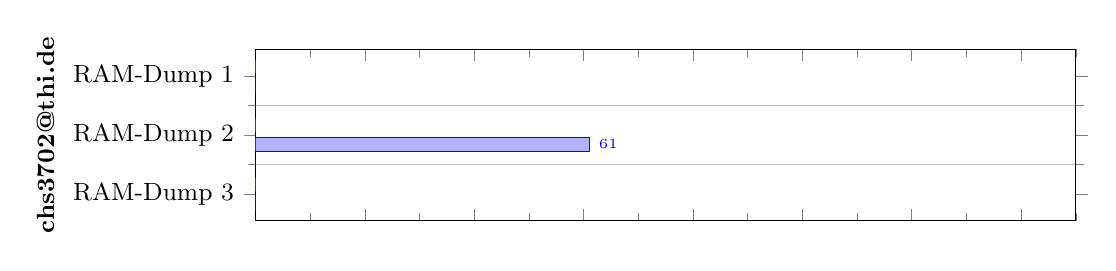
\begin{tikzpicture}
				\begin{axis}[
					xbar,
					width=12cm, 
					height=3cm, 
					ylabel style={align=center}, ylabel=\textbf{chs3702@thi.de},
					y=0.75cm,
					symbolic y coords={RAM-Dump 3, RAM-Dump 2, RAM-Dump 1},
					label style={font=\small},
					tick label style={font=\small},
					ytick=data,
					xticklabels={,,},
					xmin = 0,
					xmax = 150,
					nodes near coords, 
					nodes near coords align={horizontal},
					nodes near coords style={font=\tiny},
					nodes near coords={\pgfmathfloatifflags{\pgfplotspointmeta}{0}{}{\pgfmathprintnumber{\pgfplotspointmeta}}},
					bar width=.17cm,
					enlarge y limits={abs=2*\pgfplotbarwidth},
					scaled x ticks=false,
					legend style={
						at={(0.5,-0.1)},
						anchor=north
					},
					legend columns=3,
					yminorgrids = true,minor tick num=1
					]
					\addplot coordinates {
						(0,RAM-Dump 3) (61,RAM-Dump 2) (0,RAM-Dump 1)
					};
					\addplot coordinates {
						(0,RAM-Dump 3) (0,RAM-Dump 2) (0,RAM-Dump 1)
					};
					%				\legend{firefox.exe, Andere Prozesse}
				\end{axis}
			\end{tikzpicture}
			\\[-7pt]
			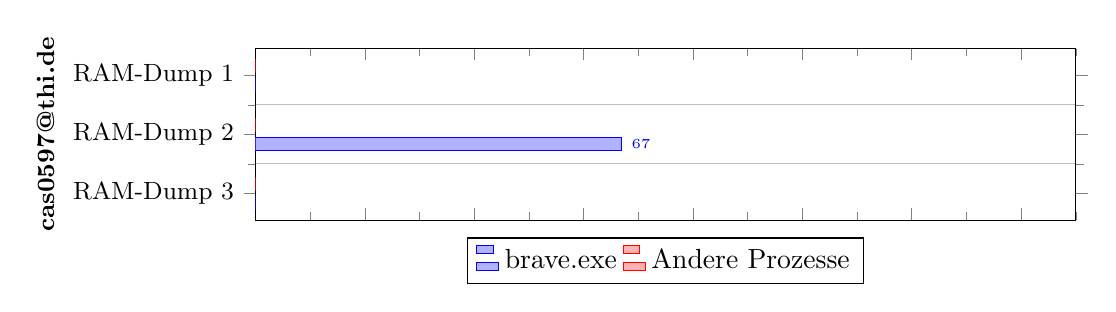
\begin{tikzpicture}
				\begin{axis}[
					xbar,
					width=12cm, 
					height=3cm, 
					ylabel style={align=center}, ylabel=\textbf{cas0597@thi.de},
					y=0.75cm,
					symbolic y coords={RAM-Dump 3, RAM-Dump 2, RAM-Dump 1},
					label style={font=\small},
					tick label style={font=\small},
					ytick=data,
					xticklabels={,,},
					xmin = 0,
					xmax = 150,
					nodes near coords, 
					nodes near coords align={horizontal},
					nodes near coords style={font=\tiny},
					nodes near coords={\pgfmathfloatifflags{\pgfplotspointmeta}{0}{}{\pgfmathprintnumber{\pgfplotspointmeta}}},
					bar width=.17cm,
					enlarge y limits={abs=2*\pgfplotbarwidth},
					scaled x ticks=false,
					legend style={
						at={(0.5,-0.1)},
						anchor=north
					},
					legend columns=3,
					yminorgrids = true,minor tick num=1
					]
					\addplot coordinates {
						(0,RAM-Dump 3) (67,RAM-Dump 2) (0,RAM-Dump 1)
					};
					\addplot coordinates {
						(0,RAM-Dump 3) (0,RAM-Dump 2) (0,RAM-Dump 1)
					};
					\legend{brave.exe, Andere Prozesse}
				\end{axis}
			\end{tikzpicture}
			%	\begin{axis}[]
				%	\legend{Logfile 1, Logfile 2}
				%	\end{axis}
			
		\end{tabular}
	}
	\caption{Anzahl gefundener E-Mail Artefakte im Brave RAM}
	\label{chart:brave-volatility-mail}
\end{table}
%TODO Vergleich mit Chrome bzgl. Anzahl der Hits entweder hier oder später

\paragraph{Yara-Regel \glqq{}DK-Logo\grqq{}}\label{chap:ergebnisse-brave-uncommon-locations-volatility-dklogo} 

Auch bei Brave wurde wieder in den Arbeitsspeicherabbildern nach den Bytes des Donaukurier-Logos gesucht. Hier kam es zu drei Treffern im zweiten RAM-Dump, was in der \autoref{chart:brave-volatility-image} zu erkennen ist.

\begin{table}[h!]
	\resizebox{\linewidth}{!}{
		\begin{tabular}{r}
			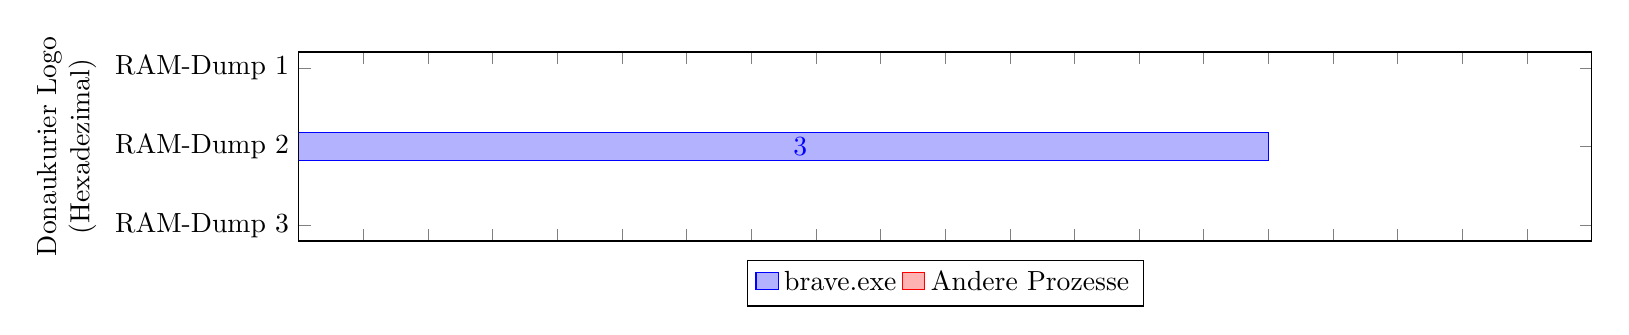
\begin{tikzpicture}
				\begin{axis}[
					xbar stacked,
					width=18cm, 
					height=12cm, 
					ylabel style={align=center}, ylabel=Donaukurier Logo\\(Hexadezimal),
					y=1cm,
					symbolic y coords={RAM-Dump 3, RAM-Dump 2, RAM-Dump 1},
					ytick=data,
					xticklabels={,,},
					xmin = 0,
					xmax = 4,
					nodes near coords, 
					nodes near coords align={horizontal},
					legend style={
						at={(0.5,-0.1)},
						anchor=north
					},
					legend columns=2
					]
					\addplot coordinates {
						(0,RAM-Dump 3) (3,RAM-Dump 2) (0,RAM-Dump 1)
					};
					\addplot coordinates {
						(0,RAM-Dump 3) (0,RAM-Dump 2) (0,RAM-Dump 1)
					};
					\legend{brave.exe, Andere Prozesse}
				\end{axis}
			\end{tikzpicture}
		\end{tabular}
	}
	\caption{Anzahl gefundener Hexadezimalwerte des Donaukurier-Logos im Brave RAM}
	\label{chart:brave-volatility-image}
\end{table}

\subsection*{Registry}\label{chap:ergebnisse-brave-uncommon-locations-registry} 

Bei der Registry konnten weder in den Process Monitor Logs noch durch die Analyse der verschiedenen Hives Artefakte gefunden werden. Weitergehende Informationen zu den Schreiboperationen und der Stringsuche in den verschiedenen Hives ist in \autoref{chap:anhang-brave-common-locations-registry} und \autoref{chap:anhang-brave-uncommon-locations-registry} zu finden.

%TODO Carl ausbessern p(f)affenhofen + computerforensik(vl)

%EOF